%%%%%%%%%%%%%%%%%%%%%%%%%%%%%%%%%%%%%%%%%%%%%%%%%%%%%%%%%%%%%%%%%%%%%%%%%%%%%%%%
%
% Template license:
% CC BY-NC-SA 3.0 (http://creativecommons.org/licenses/by-nc-sa/3.0/)
%
%%%%%%%%%%%%%%%%%%%%%%%%%%%%%%%%%%%%%%%%%%%%%%%%%%%%%%%%%%%%%%%%%%%%%%%%%%%%%%%%

%----------------------------------------------------------------------------------------
%	PACKAGES AND OTHER DOCUMENT CONFIGURATIONS
%----------------------------------------------------------------------------------------

\documentclass[
11pt, % The default document font size, options: 10pt, 11pt, 12pt
%oneside, % Two side (alternating margins) for binding by default, uncomment to switch to one side
%chapterinoneline,% Have the chapter title next to the number in one single line
spanish,
singlespacing, % Single line spacing, alternatives: onehalfspacing or doublespacing
%draft, % Uncomment to enable draft mode (no pictures, no links, overfull hboxes indicated)
%nolistspacing, % If the document is onehalfspacing or doublespacing, uncomment this to set spacing in lists to single
%liststotoc, % Uncomment to add the list of figures/tables/etc to the table of contents
%toctotoc, % Uncomment to add the main table of contents to the table of contents
parskip, % Uncomment to add space between paragraphs
%codirector, % Uncomment to add a codirector to the title page
headsepline, % Uncomment to get a line under the header
]{MastersDoctoralThesis} % The class file specifying the document structure

% mis paquetes adicionales
\usepackage[utf8]{inputenc}
\usepackage{pdflscape} % paquete para girar la hoja

%----------------------------------------------------------------------------------------
%	INFORMACIÓN DE LA MEMORIA
%----------------------------------------------------------------------------------------

\thesistitle{Sistemas de control y monitoreo para viviendas y edificios} % El títulos de la memoria, se usa en la carátula y se puede usar el cualquier lugar del documento con el comando \ttitle

% Nombre del posgrado, se usa en la carátula y se puede usar el cualquier lugar del documento con el comando \degreename
%\posgrado{Carrera de Especialización en Sistemas Embebidos} 
\posgrado{Carrera de Especialización en Internet de las Cosas} 
%\posgrado{Carrera de Especialización en Intelegencia Artificial}
%\posgrado{Maestría en Sistemas Embebidos} 
%\posgrado{Maestría en Internet de las cosas}

\author{B.Sc. Daniel Iván Cruz Flores} % Tu nombre, se usa en la carátula y se puede usar el cualquier lugar del documento con el comando \authorname

\director{Mg. Ing. Matías Alvarez (FIUBA)} % El nombre del director, se usa en la carátula y se puede usar el cualquier lugar del documento con el comando \dirname
\codirector{Nombre del codirector (pertenencia)} % El nombre del codirector si lo hubiera, se usa en la carátula y se puede usar el cualquier lugar del documento con el comando \codirname.  Para activar este campo se debe descomentar la opción "codirector" en el comando \documentclass, línea 23.

\juradoUNO{Mg. Ing. Martín Menendez (FIUBA)} % Nombre y pertenencia del un jurado se usa en la carátula y se puede usar el cualquier lugar del documento con el comando \jur1name
\juradoDOS{Mg. Ing. Christian Marcelo Yanez Flores (FIUBA)} % Nombre y pertenencia del un jurado se usa en la carátula y se puede usar el cualquier lugar del documento con el comando \jur2name
\juradoTRES{Esp. Ing. Santiago Salamandri (FIUBA)} % Nombre y pertenencia del un jurado se usa en la carátula y se puede usar el cualquier lugar del documento con el comando \jur3name

%\ciudad{Ciudad Autónoma de Buenos Aires}
\ciudad{ciudad de Buenos Aires}

\fechaINICIO{agosto de 2020}
\fechaFINAL{diciembre de 2021}


\keywords{Sistemas embebidos, FIUBA} % Keywords for your thesis, print it elsewhere with \keywordnames


\begin{document}


\frontmatter % Use roman page numbering style (i, ii, iii, iv...) for the pre-content pages

\pagestyle{plain} % Default to the plain heading style until the thesis style is called for the body content


%----------------------------------------------------------------------------------------
%	RESUMEN - ABSTRACT 
%----------------------------------------------------------------------------------------

\begin{abstract}
\addchaptertocentry{\abstractname} % Add the abstract to the table of contents
%
%The Thesis Abstract is written here (and usually kept to just this page). The page is kept centered vertically so can expand into the blank space above the title too\ldots
\centering

Esta memoria describe el diseño e implementación de un sistema automatizado para el control y monitoreo de variables de consumo energético en el hogar. El sistema se destaca especialmente por unificar resultados de una red de sensores por vía inalámbrica usando el protocolo MQTT para el servidor local y remoto. Asimismo, incluye el desarrollo de una plataforma web para visualizar resultados, un módulo de medición de temperatura, un módulo actuador, un módulo de consumo de corriente eléctrica y un servidor local.
			
En este trabajo se aplicaron conocimientos de protocolos de Internet, redes inalámbrica, base de datos relacional, desarrollo de aplicaciones web, programación orientada a objetos en Python, ciberseguridad y testing de software.	
				
\end{abstract}

%----------------------------------------------------------------------------------------
%	CONTENIDO DE LA MEMORIA  - AGRADECIMIENTOS
%----------------------------------------------------------------------------------------

\begin{acknowledgements}
%\addchaptertocentry{\acknowledgementname} % Descomentando esta línea se puede agregar los agradecimientos al índice
\vspace{1.5cm}

Quiero expresar mi gratitud a Dios por ser mi guía y acompañarme en el transcurso de mi vida, brindándome paciencia y sabiduría para culminar con éxito mis metas propuestas.

A mis padres, a mi esposa Gabriela y a mi hijo Carlos Daniel por ser mis principales pilares de vida y por haberme apoyado incondicionalmente para no decaer cuando todo parecía complicado e imposible.

A mis hermanos por estar siempre presentes, por el apoyo y el soporte moral.

A todos los docentes que con su conocimiento motivaron a desarrollarme como persona y profesional.

A mi director Matías Alvarez por su buena predisposición y orientación durante la realización del presente trabajo.

A mi amigo Sergio Cotos y a todas las personas que contribuyeron para culminar con éxito esta meta propuesta.
 

\end{acknowledgements}

%----------------------------------------------------------------------------------------
%	LISTA DE CONTENIDOS/FIGURAS/TABLAS
%----------------------------------------------------------------------------------------

\tableofcontents % Prints the main table of contents

\listoffigures % Prints the list of figures

\listoftables % Prints the list of tables


%----------------------------------------------------------------------------------------
%	CONTENIDO DE LA MEMORIA  - DEDICATORIA
%----------------------------------------------------------------------------------------

\dedicatory{\textbf{Dedicado a... [OPCIONAL]}}  % escribir acá si se desea una dedicatoria

%----------------------------------------------------------------------------------------
%	CONTENIDO DE LA MEMORIA  - CAPÍTULOS
%----------------------------------------------------------------------------------------

\mainmatter % Begin numeric (1,2,3...) page numbering

\pagestyle{thesis} % Return the page headers back to the "thesis" style

% Incluir los capítulos como archivos separados desde la carpeta Chapters

% Chapter 1

\chapter{Introducción general} % Main chapter title

\label{Chapter1} % For referencing the chapter elsewhere, use \ref{Chapter1} 
\label{IntroGeneral}
Para entender este trabajo es necesario describir ciertos conceptos, explicarlos y comparar herramientas para conocer cuáles nos ofrecen mejores prestaciones para el desarrollo de una solución tecnológica en la gestión eficiente de la energía eléctrica. 
%----------------------------------------------------------------------------------------

% Define some commands to keep the formatting separated from the content 
\newcommand{\keyword}[1]{\textbf{#1}}
\newcommand{\tabhead}[1]{\textbf{#1}}
\newcommand{\code}[1]{\texttt{#1}}
\newcommand{\file}[1]{\texttt{\bfseries#1}}
\newcommand{\option}[1]{\texttt{\itshape#1}}
\newcommand{\grados}{$^{\circ}$}

%----------------------------------------------------------------------------------------

%\section{Introducción}

%----------------------------------------------------------------------------------------
\section{Motivación}
Al encender cualquier dispositivo eléctrico u electrónico se produce un consumo de energía eléctrica que normalmente se desconoce. Simplemente a final de mes, se recibe la factura de consumo eléctrico, donde se indica el consumo mensual y el monto a pagar. A muchas de las empresas que tienen procesos industriales les ocurre lo mismo y es que el control del consumo de manera precisa no está normalizado en el ámbito doméstico (\emph{smart home}) y sigue siendo un aspecto aun por mejorar. Este control es muy importante ya que gracias a él podemos mejorar la eficiencia energética, ahorrando dinero para una familia o una empresa y a la vez siendo respetuosos con el medio ambiente.

Bajo ese contexto antes y durante la pandemia por el Covid-19, se registraron miles de quejas por montos excesivos en los recibos de energía eléctrica en muchos departamentos en el país de Perú. Antes de la pandemia, una usuaria de Luz del Sur pagaba 80 soles al mes (\$20 USD al cambio actual) por el servicio de energía eléctrica en su vivienda en la ciudad de Lima. Ahora, pretenden cobrarle 180 soles por mes (\$45 USD al cambio actual). Cuando el usuario quiso reclamar, la empresa responsable de brindar el servicio no le contestaba. Algo parecido le pasó a una asociación de comerciantes a la que, a pesar de que su establecimiento estaba cerrado desde el 16 de marzo del 2020, La empresa EDELNOR pretende cobrarle 250 soles (\$ 62 USD al cambio actual) por consumos no realizados durante el mes. Estos son algunos de los miles de denuncias de consumidores que se han hecho públicas en el país de Perú  \citep{WEBSITE:1}.

Entre el 16 de marzo y fines de junio de 2020, cuando el Gobierno peruano declaró el Estado de Emergencia Nacional por el COVID-19, las empresas generadoras de electricidad dejaron de enviar a su personal a las viviendas para realizar la lectura de los consumos en los medidores de energía eléctrica de los predios y facturaron por el consumo promedio de los seis meses anteriores. En muchos casos se encontró que los consumos normales habían crecido enormemente, en otros se duplicaron y hasta se triplicaron. Este aparente sinceramiento de los consumos generó miles de reclamos por cobros excesivos como se ilustra con la figura \ref{fig:noticia}. 

El mayor número de reclamos de los usuarios se presentó en julio y agosto de 2020. En solo una semana, el Organismo Supervisor de la Inversión en Energía y Minería (OSINERGMIN) recibió en Lima alrededor de 20 mil reclamos, tanto contra ENEL como por LUZ DEL SUR. Esta situación se repitió a nivel nacional, sobre todo en las regiones de Puno, La Libertad, Áncash y Ucayali \citep{WEBSITE:1}.

%\vspace{1cm}
\begin{figure}[htbp]
\centering
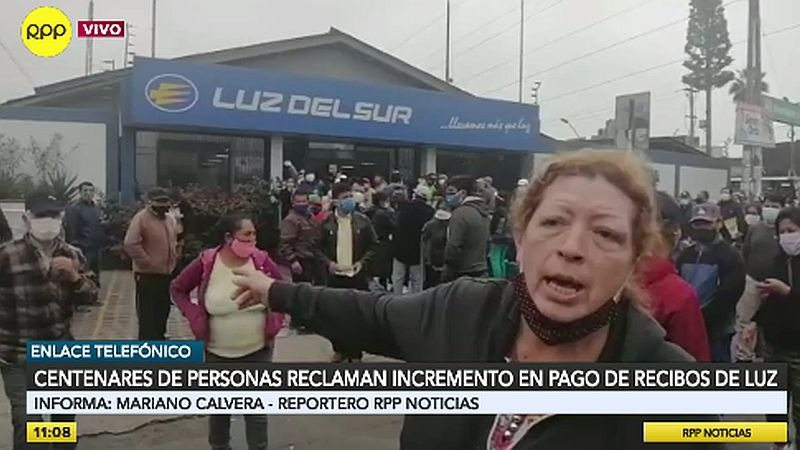
\includegraphics[width=.7\textwidth]{./Figures/motivacion.jpg}
\caption{Noticias de la problemática en Lima Perú \protect\footnotemark.}
\label{fig:noticia}
\end{figure}
%\vspace{1cm}
\footnotetext{Imagen tomada de \url{https://rpp.pe/noticias/luz-del-sur}}

El organismo supervisor del estado recordó que en los casos donde la lectura del medidor confirme que el consumo real ha sido menor al facturado, la empresa deberá devolver lo pagado en exceso en una sola oportunidad o proceder a refacturar \citep{WEBSITE:2}.

Realizar el proceso de refacturación para corregir estos errores costará demasiado tiempo y dinero al estado y a las empresas que ofrecen dicho servicio, presentando incomodidad y daño económico a toda la población afectada. 

Como parte de los usuarios afectados en esta problemática en Perú, surge la necesidad de desarrollar un sistema de monitoreo y control que permita conocer el consumo eléctrico mensual detallado, siendo este una herramienta automatizada de respaldo y que sirva como evidencia para prevenir facturaciones erróneas para hogares, edificios habitacionales, empresas, etc.


\section{Identificación y análisis}



\subsection{Propósito}

El propósito de este proyecto es diseñar y desarrollar un sistema informático capaz de controlar y monitorear viviendas u otros ambientes mediante el protocolo MQTT para brindar una gestión inteligente respecto a confort y consumo energético.

\subsection{Alcance}

El proyecto incluye los siguientes ítems:
\begin{itemize}
\item Diseño y desarrollo de un módulo principal local.
\item Diseño y desarrollo del módulo replicador de datos local-nube.
\item Diseño y desarrollo del módulo actuador y de consumo.
\item Diseño y desarrollo del módulo de control de temperatura.
\end{itemize}

\subsection{Objetivos}
\begin{itemize}
\item Diseñar y desarrollar un sistema IoT para medir el consumo eléctrico.
\item Diseñar y desarrollar un sistema que no dependa de una conexión a Internet para su funcionamiento.
\item Diseñar y desarrollar un \emph{software} a medida para la gestión de control y monitoreo de una vivienda o edificio.
\item Diseñar e implementar módulos con comunicación Wi-Fi para el control y monitoreo de energía eléctrica.
\end{itemize}
%----------------------------------------------------------------------------------------

\section{Estado del arte}

A continuación, se describen soluciones que son utilizadas en el control del consumo eléctrico y que están actualmente en el mercado comercial. 

Para una mejor comprensión se los clasifica en dos categorías:

\begin{itemize}
\item Sistemas de monitoreo para gestión de energía eléctrica.
\item Módulos independientes para gestión de energía eléctrica.
\end{itemize} 

\subsection{Sistemas de monitoreo para gestión de energía eléctrica}
Los sistemas de monitoreo son sistemas integradores automatizados compuestos por un \emph{software} de control y monitoreo, sensores y actuadores, por ejemplo:

\begin{itemize}
\item \keyword{Energy Vision}: solución de \emph{software} para gestión del consumo de energía. Energy vision - Centraline es una nueva herramienta de \emph{software} de gestión energética profesional con el fin de lograr un ahorro importante y maximizar la eficiencia energética. El sistemas se ilustra con la figura \ref{fig:energy-vision} 
%\vspace{0.5cm}
\begin{figure}[htbp]
\centering
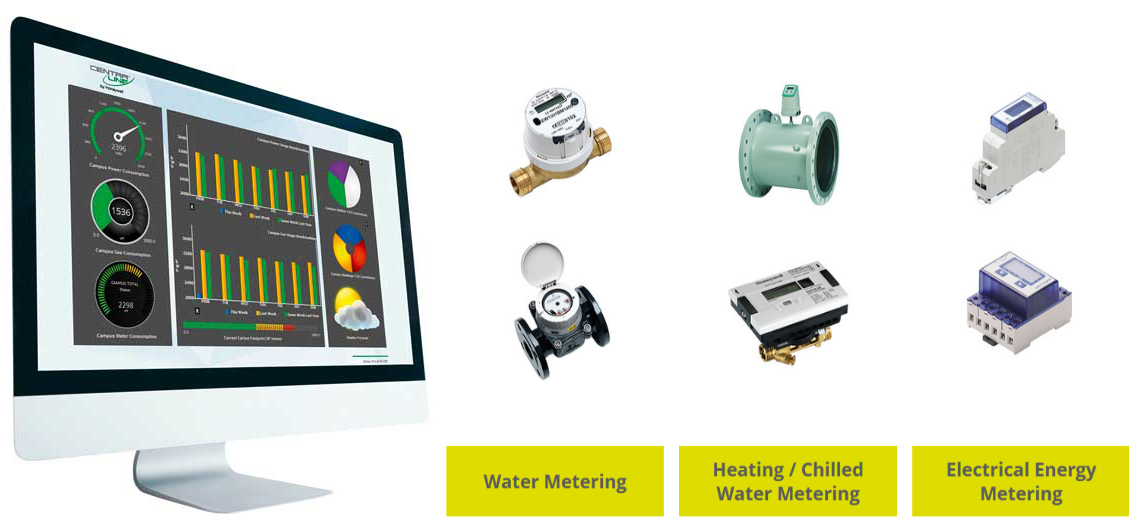
\includegraphics[width=.9\textwidth]{./Figures/energy-vision.jpg}
\caption{Sistema y productos Energy Vision \protect\footnotemark}
\label{fig:energy-vision}
\end{figure}

\footnotetext{Imagen tomada de \url{https://www.centraline.com/itIT/prodotti-e-documentazione/special/energy-vision-nx.html}}


El \emph{software} permite recopilar y analizar todas las formas de uso de energía para una gestión energética profesional y constituye un componente esencial en la automatización de edificios eficientes desde el punto de vista energético \citep{WEBSITE:13}. Esta herramienta de \emph{software} contiene gráficos y diagramas visualmente atractivos y proporcionan una presentación ordenada y fácil de comprender de la información que se necesita. Recopila, archiva, evalúa y consulta todos los datos de un edificio. 

Se puede acceder al sistema desde todo tipo de dispositivos mediante un navegador con Internet.

%\vspace{1cm}
%\vspace{1cm}

\item \keyword{Iammeter}: sistema de monitoreo de energía.

Iammeter es un sistema de monitoreo de energía dedicado, al que se puede conectar medidores de energía Wi-Fi y luego comenzar a rastrear el uso de electricidad de su hogar o edificio comercial, y monitorear el flujo de energía del sistema fotovoltaico solar \citep{WEBSITE:11}.

El sistema Iammeter puede generar un análisis integral del consumo de energía por usuarios, ofreciendo gráficos de datos y algunos detalles en el panel de información general. Ofrece el cálculo de la factura de la luz diaria/mensual y monitoreo en tiempo real del uso de electricidad \citep{WEBSITE:12}. El sistema se ilustra con la figura \ref{fig:iammeter}.

\vspace{0.5cm}

\begin{figure}[htbp]
	\centering
	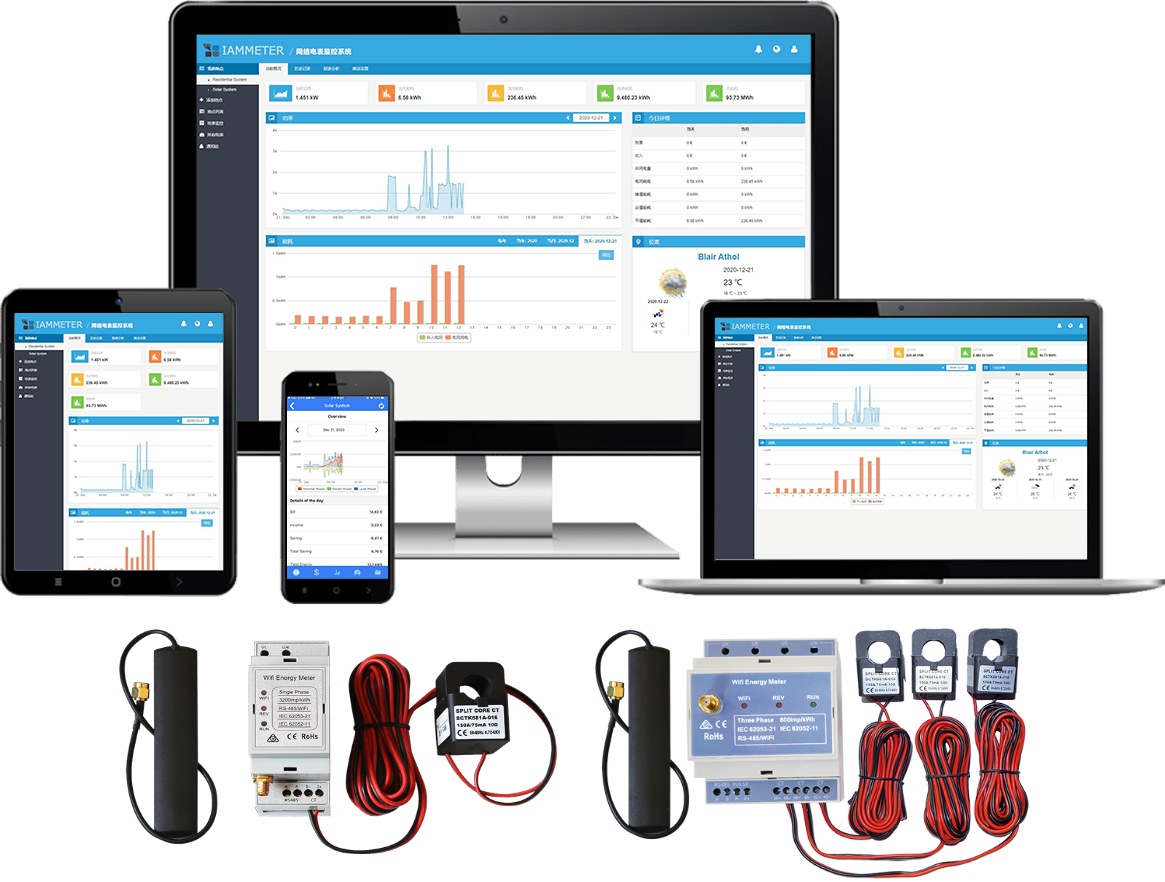
\includegraphics[width=.9\textwidth]{./Figures/iammeter.png}
	\caption{Sistema y productos Iammeter \protect\footnotemark.}
	\label{fig:iammeter}
\end{figure}
\vspace{0.5cm}

\footnotetext{Imagen tomada de \url{https://es.iammeter.com/}}

Se puede acceder sistema desde todo tipo de dispositivos mediante un navegador con Internet o mediante su aplicación móvil.
\vspace{1cm}
\vspace{1cm}

\item \keyword{Bee2energy}: gestión de eficiencia energética.

El sistema Bee2energy de la empresa Compta ofrece un servicio integral de \emph{software} que permite a las empresas e instituciones lograr mejoras significativas en el uso de la eficiencia energética a la vez que minimiza los impactos ambientales, reduciendo los consumos y los costos operativos \citep{WEBSITE:14}. El sistema se ilustra con la figura \ref{fig:bee2energy}. 

\begin{figure}[htbp]
	\centering
	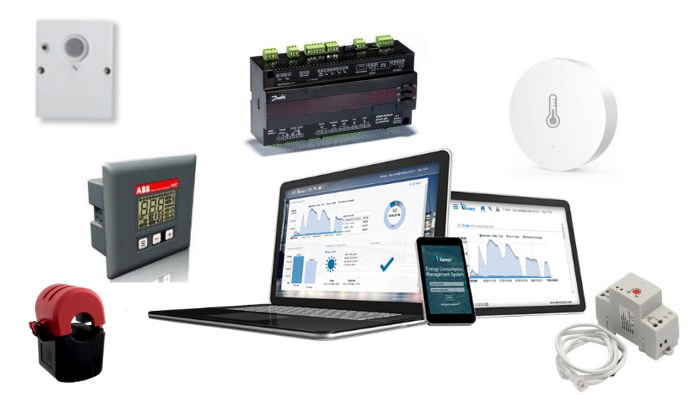
\includegraphics[width=.8\textwidth]{./Figures/bee2energy.jpg}
	\caption{Sistema y productos Bee2energy \protect\footnotemark.}
	\label{fig:bee2energy}
\end{figure}

\footnotetext{Imagen tomada de \url{https://www.ceb-solutions.com/es/productos/bee2energy/}}

Bee2energy es una solución IoT basada en la nube a la que se puede acceder en cualquier momento y en cualquier lugar a través de Internet. Brinda operaciones en tiempo real con un modelo de negocio SaaS (\emph{\emph{software} as a service}) flexible y con capacidad multicanal \citep{WEBSITE:14}. Las funciones de control en edificios se ilustra con la figura \ref{fig:bee2energy2}.

\begin{figure}[htbp]
	\centering
	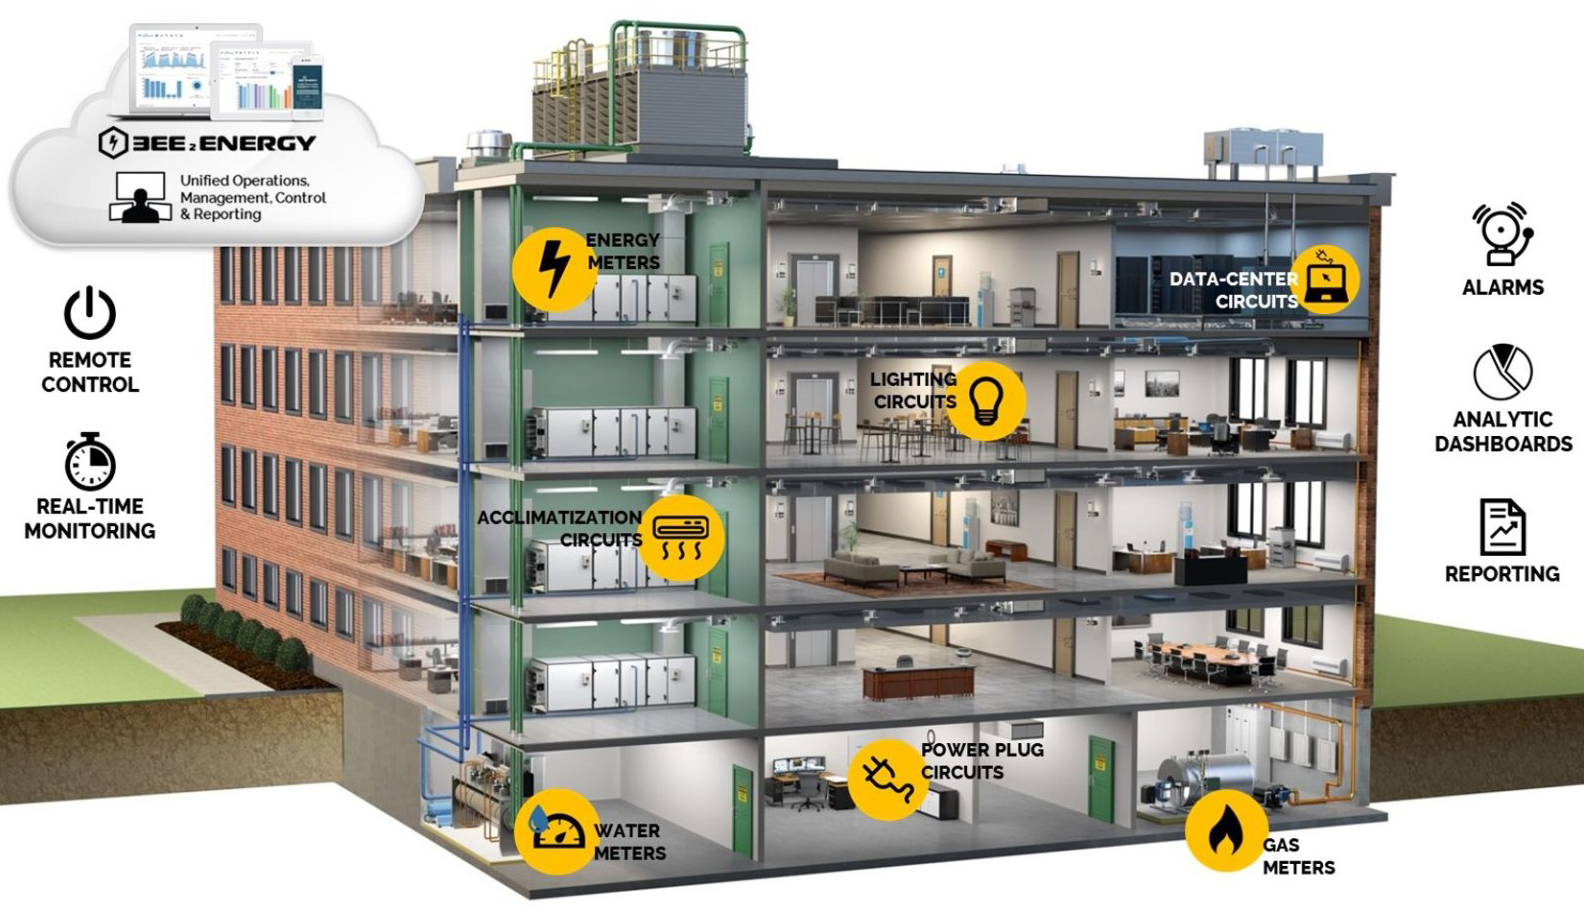
\includegraphics[width=.85\textwidth]{./Figures/bee2energy2.jpg}
	\caption{Monitoreo y control en tiempo real en edificios \protect\footnotemark.}
	\label{fig:bee2energy2}
\end{figure}

\footnotetext{Imagen tomada de \url{https://www.ceb-solutions.com/es/productos/bee2energy/}}

Ofrece monitoreo en tiempo real de consumos, temperaturas, humedad y otros indicadores, configuración de reglas y encender / apagar equipos automáticamente o configurar alarmas y notificaciones.
\end{itemize}
%----------------------------------------------------------------------------------------
\subsection{Módulos independientes para gestión de energía eléctrica}
Los módulos independientes son sensores o actuadores  que se comercializan de forma individual, puede ser un sensor de consumo, interruptores o tomacorrientes inteligentes, por ejemplo: 
\begin{itemize}

\item \keyword{Tomacorriente smart}: es la manera más sencilla de convertir en inteligentes tus dispositivos electrónicos para poder controlarlos. Simplemente se debe conectar en un tomacorriente de CA (corriente alterna) e integrarlo a la red Wi-Fi existente, no requiere un concentrador y a través de una aplicación, puedes encender y apagar las luces o electrodomésticos en forma remota desde cualquier lugar. Por ejemplo el dispositivo de la figura \ref{fig:tomacorriente}.

\begin{figure}[htbp]
	\centering
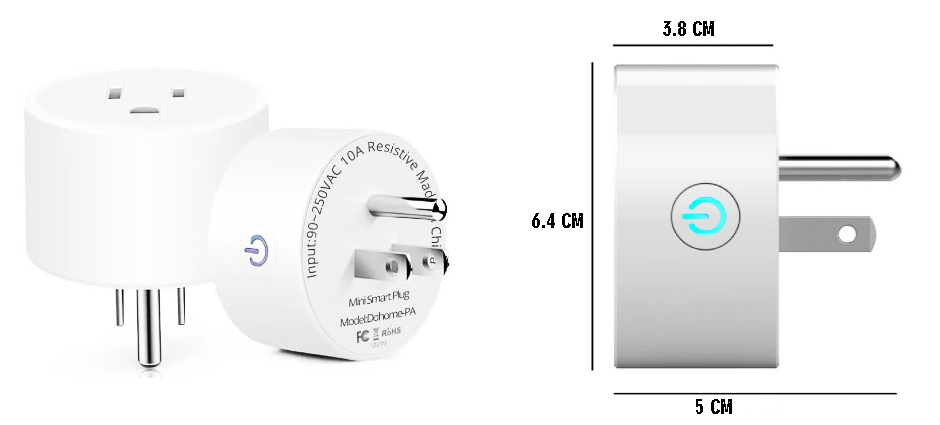
\includegraphics[width=0.8\textwidth]{./Figures/tomacorriente.png}
	\caption{Tomacorriente inteligente de facil uso \protect\footnotemark.}
	\label{fig:tomacorriente}
\end{figure}

\footnotetext{Imagen tomada de \url{https://www.promart.pe/electricidad/interruptores-y-tomacorrientes/}}

%\vspace{1cm}
%\vspace{1cm}
%\vspace{1cm}
%\vspace{1cm}
%\vspace{1cm}
%\vspace{1cm}
%\vspace{1cm}
%\vspace{1cm}



\item \keyword{Medidor digital eléctrico monofásico}: es un medidor tipo electrónico con cubierta de policarbonato diseñado para controlar el consumo de energía de manera independiente, tiene una alta resistencia a la humedad, corrosión y temperatura. Por ejemplo el dispositivo de la figura \ref{fig:medidor}.

\begin{figure}[htbp]
	\centering
	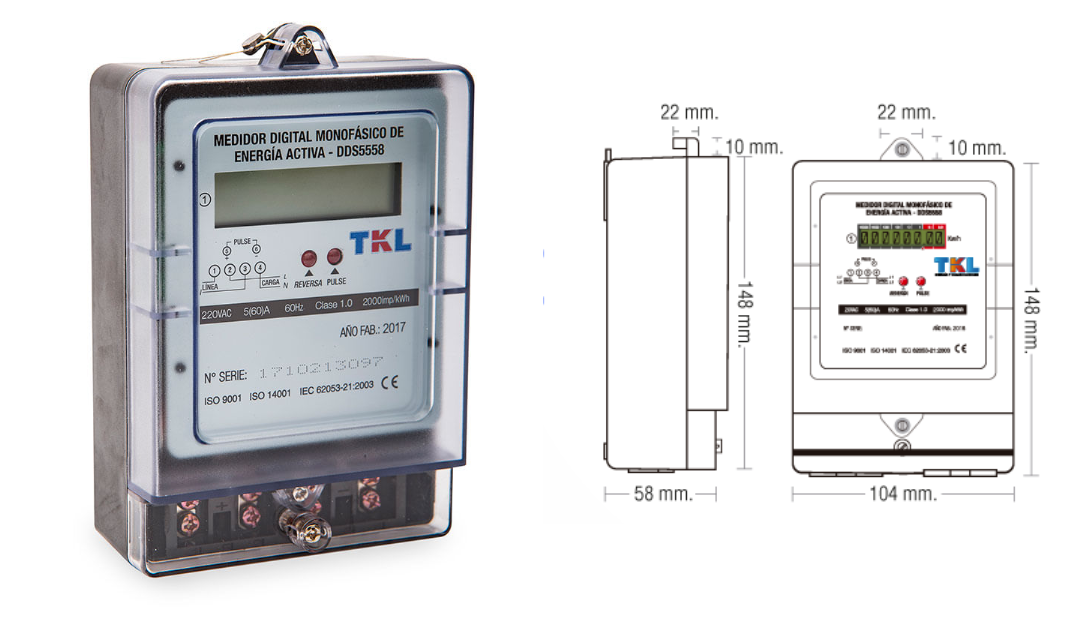
\includegraphics[width=0.9\textwidth]{./Figures/medidor.png}
	\caption{Medidor digital monofásico \protect\footnotemark.}
	\label{fig:medidor}
\end{figure}

\footnotetext{Imagen tomada de \url{https://www.promart.pe/medidor-digital-ciclometrico-60-amperios/}}

Es un medidor que incluye una pantalla LCD donde muestra la lectura de watts utilizados dentro de una vivienda, negocio u oficina.

\end{itemize}

\subsection{Comparación entre soluciones}

La comparación entre las distintas soluciones mencionadas se muestran en las tablas \ref{tab:tabla1}, \ref{tab:tabla2},  \ref{tab:tabla3} y \ref{tab:tabla4}, considerando aspectos más relevantes para conocer sus principales diferencias según su categoría. 
\begin{itemize}
\item Sistemas de monitoreo para gestión de energía eléctrica:

%%%%%%%%%%%%%%%%%%%%%%%%%%%%%%%%%%
\begin{table}[h]
	\centering
	\caption[Comparativa de soluciones entre producto y sector]{Comparativa producto y sector}
	\begin{tabular}{l c c }    
		\toprule
		\textbf{Empresa} 	& \textbf{Producto} & \textbf{Sector}  \\
		\midrule
		Honeywell International Inc & Energy Vision & Energético \\		
		Beijing Lewei IOT Technologies Co. Ltd.	 & Iammeter	& Energético solar \\
		Compta Energing Business	 & Bee2energy	& Energético \\
		\bottomrule
		\hline
	\end{tabular}
	\label{tab:tabla1}
\end{table}


%%%%%%%%%%%%%%%%%%%%%%%%%%%%%%%%%%%%%%
%escribir texto 2

\begin{table}[h]
	\centering
	\caption[Comparativa de soluciones entre acceso y servidor]{Comparativa acceso y tipo de servidor}
	\begin{tabular}{l c c c c }    
		\toprule
		\textbf{Producto} & \textbf{Acceso}  & \textbf{uso} & \textbf{S. local}   & \textbf{S. remoto} \\
		\midrule
		Energy Vision & Local y remoto 	& Navegador & No & Si  \\		
		Iammeter	 & Local y remoto	& Navegador y App. & No & Si  \\
		Bee2energy	 & Local y remoto	& Navegador & No & Si  \\
		\bottomrule
		\hline
	\end{tabular}
	\label{tab:tabla2}
\end{table}

%\vspace{1cm}
%\vspace{1cm}

%%%%%%%%%%%%%%%%%%%%%%%%%%%%%%%%%%%

%escribir texto 3

\begin{table}[h]
	\centering
	\caption[Comparativa de soluciones entre protocolo y hardware]{Comparativa protocolo y tipos de hardware}
	\begin{tabular}{l p{5cm} p{5cm}}    
		\toprule
		\textbf{Producto} 	 & \textbf{Protocolo}  & \textbf{Sensores y actuadores}  \\
		\midrule
		Energy Vision & Modbus, M-Bus  y TCP/IP 	& Propios \\		
		Iammeter	 & MQTT y TCP/IP	& Propios y compatibles con       dispositivos Sonoff   \\
		Bee2energy	 & Múltiples protocolos IoT		& Propios y compatibles con otros comerciales  \\
		\bottomrule
		\hline
	\end{tabular}
	\label{tab:tabla3}
\end{table}


\item Módulos independientes para gestión de energía eléctrica:


\begin{table}[h]
	\centering
	\caption[Comparativa de módulos entre protocolo y hardware]{Comparativa protocolo y tipos de hardware}
	\begin{tabular}{l p{2cm} p{3cm} p{2cm}}    
		\toprule
		\textbf{Producto} 	 & \textbf{Protocolo}  & \textbf{Función} & \textbf{Acceso} \\
		\midrule
		Tomacorriente smart & TCP/IP (Wi-Fi)	& Interruptor inteligente. & App. móvil  \\		
		Medidor digital eléctrico	 & -	& Registro de consumo.  & Presencial visual \\
		
		\bottomrule
		\hline
	\end{tabular}
	\label{tab:tabla4}
\end{table}



\end{itemize}

\section{Conceptos generales}

En esta sección se describen aspectos esenciales para poder conocer y entender las tecnologías y servicios usados en el trabajo.

\subsection{IoT y computación en la nube}

Internet de las Cosas (IoT) y la computación en la nube (\emph{Cloud Computing}) son dos conceptos y soluciones que cada día ocupan una mayor importancia en el desarrollo tecnológico industrial y empresarial, pero antes de abordar su rol e importancia es importante definirlas:



\begin{itemize}
\item Internet de las Cosas (IoT): hace referencia a una tecnología basada en la conexión de objetos cotidianos a Internet que intercambian, agregan y procesan información sobre su entorno físico para proporcionar servicios de valor añadido a los usuarios finales. También reconoce eventos o cambios, y tales sistemas pueden reaccionar de forma autónoma y adecuada \citep{BOOK:1}.

IoT es un conjunto de tecnologías que facilita la integración de sensores y actuadores que nos informan del estado de elementos cotidianos, como electrodomésticos, vehículos, herramientas o incluso seres vivos. Nos permite interactuar con ellos, habilitando su conectividad con plataformas en la nube que reciben y procesan la información para, tras su análisis, poder tomar decisiones.

\item Cloud Computing: la computación en la nube como paradigma proporciona a las empresas y usuarios necesidades informáticas (como \emph{software}, almacenamiento de datos, capacidad de procesamiento, etc.) a través de internet que son fácilmente escalables bajo demanda. Los documentos, correos electrónicos y otros datos, así como las aplicaciones informáticas, se almacenarán ``en la nube'', es decir, en línea, de modo que se puede acceder a los mismos desde cualquier ordenador o dispositivo móvil \citep{BOOK:1}.

La generalización del \emph{Cloud Computing} en la infraestructura TIC (tecnologías de información y comunicación) habilita la viabilidad de ejecutar aplicaciones completamente en Internet. En particular, permite flexibilidad de acceso \citep{BOOK:1}.

La computación en la nube es una tecnología que permite acceso a \emph{software}, almacenaje de ficheros y procesamiento de datos a través de Internet, siendo una opción alternativa a la ejecución en un servidor local. 

En el modelo de nube, no es necesario instalar aplicaciones de forma local en computadoras.

\end{itemize}

\subsection{Sensores y redes inalámbricas}

En la revolución de la industria conectada (Industria 4.0) cada vez existe una mayor oferta de sensores inteligentes que, además de medir la magnitud en cuestión, llevan integrado un circuito electrónico compatible con los estándares de comunicaciones más habituales en el mundo de IoT. Capturar datos y métricas siempre ha sido una necesidad en el mundo de los procesos y operaciones industriales.

\begin{itemize}
\item Sensores: son dispositivos capaces de convertir el mundo real (físico/químico) en el mundo digital (electrónico), nos permiten llevar la realidad a una dimensión que podemos gestionar para finalmente tomar decisiones e, incluso, actuar sobre el propio entorno. Son equipos que convierten la magnitud de entrada (temperatura, humedad, nivel, presión, etc.) en una señal eléctrica medible e interpretable por los dispositivos electrónicos.

\item Redes inalámbricas: las redes inalámbricas (\emph{Wireless}) logran propagar la conexión entre dispositivos a través de medios no físicos, usan diferentes tecnologías como las ondas electromagnéticas, radiación y medios ópticos para su transferencia. Existen varios tipos de redes inalámbricas con diferentes alcances y funcionalidades.

\end{itemize}

\subsection{Tipos de redes de IoT}

Podemos clasificarlas en dos categorías:
\begin{enumerate}
\item Redes de corto alcance y bajo consumo 

Las redes de baja potencia y corto alcance están indicadas para hogares, oficinas y otros entornos de reducido tamaño. Normalmente, necesitan baterías pequeñas y su usó suele resultar económico \citep{WEBSITE:15}. Por ejemplo:

\begin{itemize}
\item Bluetooth
\item Z-Wave
\item NFC
\item ZigBee
\item Wi-Fi/802.11
\end{itemize}

%\vspace{1cm}

\item Redes de área extensa de bajo consumo (LPWAN)

Las redes LPWAN permiten la comunicación en un radio mínimo de 500 metros, tienen un consumo de energía mínimo y se usan para la mayoría de los dispositivos IoT \citep{WEBSITE:15}. 

Los siguientes son algunos ejemplos comunes de redes LPWAN:

\begin{itemize}
\item 4G LTE para IoT
\item 5G para IoT
\item Cat-0
\item Cat-1
\item LoRaWAN
\item LTE Cat-M1
\item Sigfox
\item Banda estrecha o NB-IoT/Cat-M2
\end{itemize}

\end{enumerate}

\vspace{0.5cm}

La distancia a la que los datos deben viajar (corta o larga) determina el tipo de conectividad necesaria para un proyecto de IoT.

%----------------------------------------------------------------------------------------
\let\cleardoublepage\clearpage % para eliminar pagina en blanco siguiente
\chapter{Introducción específica} % Main chapter title

\label{Chapter2}

%----------------------------------------------------------------------------------------
%	SECTION 1
%----------------------------------------------------------------------------------------
%En este capítulo se presentan las tecnologías utilizadas e incorporadas en este trabajo. 

En este capítulo se explica el funcionamiento general del sistema implementado y se brinda una introducción a las diferentes tecnologías utilizadas en este trabajo.

\section{Funcionamiento general del sistema}

Este trabajo presenta una propuesta de solución a partir del desarrollo de un prototipo mínimo viable de un sistema IoT para integrar, centralizar y unificar resultados de una red de sensores y actuadores, mediante un sistema web de monitoreo y control, así como la construcción de módulos propios para dicha tarea, sin la necesidad de una conexión a Internet para su funcionamiento. 

Todos estos componentes trabajan en conjunto para brindar al cliente una solución tecnológica que sirva como herramienta visualmente amigable y que pueda ser el soporte en las tareas de gestión de consumo eléctrico. Para lograrlo, se desarrollaron módulos que integran \emph{software} y \emph{hardware}, estos hacen posible la adquisición de datos de sensores y actuadores ubicados en distintos puntos de una vivienda, conectados a una red local vía Wi-Fi. Cada lectura de los sensores permite el envío de datos a un servidor central local mediante el protocolo MQTT por vía inalámbrica, siendo el módulo principal local el responsable de registrar los valores de los sensores ante cualquier corte de Internet. La figura \ref{fig:diagrama1} ilustra el diagrama de componentes del sistema y la lógica de conexión.

\begin{figure}[htbp]
	\centering
	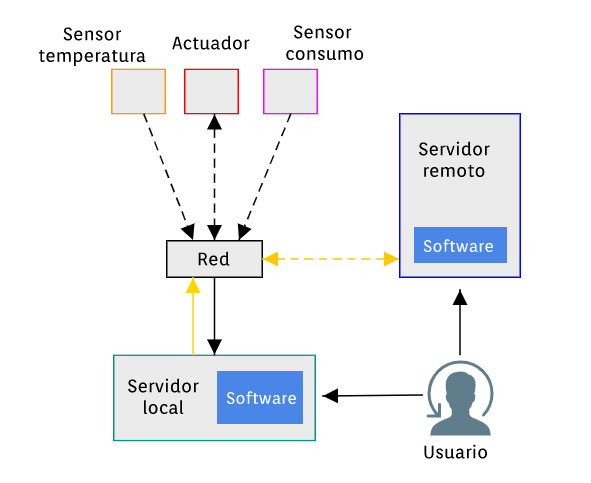
\includegraphics[width=0.9\textwidth]{./Figures/bloques.png}
	\caption{Diagrama de bloques del sistema.}

	\label{fig:diagrama1}
\end{figure}

El sistema tiene la capacidad de permitir el acceso por medio de cualquier dispositivo que cuente con un navegador web y con conectividad a Internet a cualquier usuario, ya sea desde dentro de la red local o desde fuera. Para alcanzar esta funcionalidad, fue necesario desarrollar un módulo de \emph{software} que permita la replicación de datos desde la red local hacia un broker remoto ubicado en la nube. La necesidad de replicación de los datos hacia la nube solo se da mientras exista conexión a Internet. Para los casos de corte de Internet, el módulo replicador enviará los datos de forma automática la próxima vez que detecte el servicio.% de conexión a Internet. 

Los componentes claves dentro de la solución propuesta y que se integran en la arquitectura IoT usada en el proceso de desarrollo son: 


\begin{itemize}
\item Dispositivos IoT: son los módulos diseñados a partir de la integración de \emph{software}, \emph{firmware} y \emph{hardware}; es posible conectarlos de forma inalámbrica a una red más amplia.
\item Redes: los routers domésticos, puntos de acceso y las configuraciones de las redes o las puertas de enlaces son los responsables de conectar varios dispositivos IoT a la nube.
\item Servidor local: es aquel servidor instalado con el fin de trabajar \emph{offline} y \emph{online}. Es una alternativa útil cuando existe corte del servicio de Internet. El servidor local es el módulo que contiene el broker MQTT. 
\item Nube: servidores remotos en centros de datos que consolidan y almacenan la información con seguridad. Son servicios utilizados en el trabajo para garantizar el acceso remoto de usuarios al sistema.
\end{itemize}

\section{Servicios en la nube}

El \emph{Cloud Computing} o servicios en la nube cobra cada vez más relevancia en las empresas debido, principalmente, a la ventaja de no tener que hacer grandes inversiones en infraestructuras que mantengan aplicaciones, plataformas o servidores propios.

Los servicios en la nube se clasifican en:

\begin{itemize}
\item Infraestructura como servicio (IaaS): esta categoría ofrece servicios de infraestructura, entre ellos está la distribución de recursos de computación y almacenamiento cuyos precios varían de acuerdo al consumo realizado. Las empresas que los contratan nunca ven el equipo físico, pero sí pueden tener acceso a ellos al momento de usar el servicio deseado \citep{BOOK:2}.

%Ejemplo de IaaS:

%\begin{itemize}
%\item Amazon Web Services
%\item Microsoft Azure
%\item Google Cloud Platform
%\end{itemize}

%\vspace{0.5cm}

\item Plataforma como servicio (PaaS): este servicio ofrece plataformas de desarrollo sin necesidad de adquirir tecnología de costo muy elevado. El \emph{hardware} y el \emph{software} en este modelo es administrado por el proveedor del servicio, además de que los desarrolladores no se preocupan por el rendimiento del hardware ni por las actualizaciones del sistema, ya que todo lo realiza el proveedor \citep{BOOK:2}.
 
%Ejemplos de PaaS:

%\begin{itemize}
%\item AWS Elastic Beanstalk
%\item Azure App Service
%item Google App Engine

%\end{itemize}

%\vspace{0.5cm}


\item \emph{Software} como servicio (SaaS): constituye el modelo más utilizado porque, además de brindar servicio de \emph{software}, ofrece también el almacenamiento de la información. Este modelo permite simplicidad de integración y escalabilidad \citep{BOOK:2}. 

%Ejemplos de SaaS:

%\begin{itemize}
%\item Microsoft Office 365
%\item Aplicaciones web de Google
%\end{itemize}

%\vspace{0.5cm}

\end{itemize}

En la figura \ref{fig:servicios} se muestra una representación gráfica para diferenciar las capas y su orientación para cada modelo de servicio.



%\vspace{1.5cm}

\begin{figure}[htbp]
	\centering
	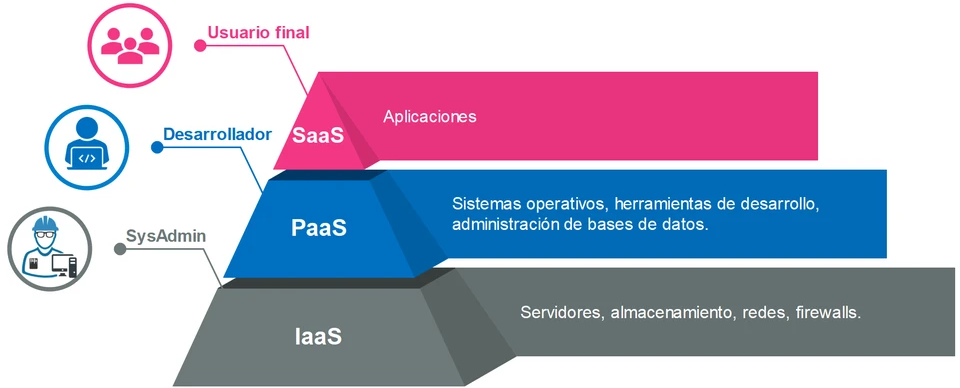
\includegraphics[width=0.8\textwidth]{./Figures/servicios.png}
	\caption{Tipos de servicio y orientación por rol \protect\footnotemark.}

	\label{fig:servicios}
\end{figure}

\footnotetext{Imagen tomada de \url{https://openwebinars.net/blog/tipos-de-cloud-computing/}}

%\vspace{1cm}

Para el trabajo se usó el servicio tipo PaaS en la creación y configuración del broker remoto así como para el almacenamiento de la aplicación web y para la gestión de la base de datos.


%Para el trabajo se consideró el servicio de \emph{cloud computing} tipo PaaS, porque permite la creación y configuración del broker remoto, el servidor Apache para la aplicación web y el gestor de base de datos MySQL.

El plan utilizado se divide en dos categorías, la primera está definida por el servicio del servidor web para alojar la aplicación web de monitoreo y control (réplica) y la segunda por el servicio del broker remoto que permite la comunicación directa con el broker local. La comunicación entre ambos servicios se hace mediante el protocolo MQTT utilizando la biblioteca  \emph{Eclipse Paho JavaScript Client}, se puede encontrar mayor información en su página oficial \citep{WEBSITE:41}. 

Las principales características  del servicio contratado para la implementación del sistema de monitoreo se muestran en la tabla \ref{tab:serverweb} y las características del servicio para el broker remoto se muestran en la tabla  \ref{tab:brokerremoto}.


\begin{table}[h]
	\centering
	\caption[Características del servicio en la nube]{Características del servicio en la nube.}
	\begin{tabular}{p{7cm} p{5cm} }    
		\toprule
		\textbf{Característica} 	 & \textbf{Detalle}  \\
		\midrule
		Sistema operativo  & GNU/Linux Centos\\		
		Espacio de almacenamiento & 1000 MB \\
		Transferencia mensual  & 10 GB\\				
		Cantidad base de datos 	  & ilimitados\\
		Acceso FTP 	  & sí\\
		Backup diario y semanal 	  & sí\\
		Soporte 24/7 	  & sí\\
		Seguridad - Firewall	  & sí\\
		Certificados SSL/TLS	  & sí\\
		PHP	  & V7 y V8\\
		MySQL y	phpMyAdmin  & sí\\
		Cron Jobs	  & sí\\
		\bottomrule
		\hline
	\end{tabular}
	\label{tab:serverweb}
\end{table}

%%%%%%%%%%%%%%%%%%%%%%%%%%%%%%%%%%%%%%%%%%%%%%%%%%%%%

\begin{table}[h]
	\centering
	\caption[Características del broker remoto]{Características del broker remoto.}
	\begin{tabular}{p{5cm} p{7cm} }    
		\toprule
		\textbf{Característica} 	 & \textbf{Detalle}  \\
		\midrule
		Conexiones activas  & 200\\		
		Mensajes por segundo & 10 k \\
		Interface  & MQTT interface, HTTP interface\\		
		Compatibilidad & arduino, javaScript, processing, ruby \\		
		Deployment 	  & por instancias\\
		Envíos y recepción de datos & objetos codificados JSON\\
		
		\bottomrule
		\hline
	\end{tabular}
	\label{tab:brokerremoto}
\end{table}




%En la figura \ref{fig:capas-servicios} se muestran las capas de cada servicio descrito y el acceso que el cliente tiene con cada modelo (capas de color verde).

%\begin{figure}[htbp]
%	\centering
%	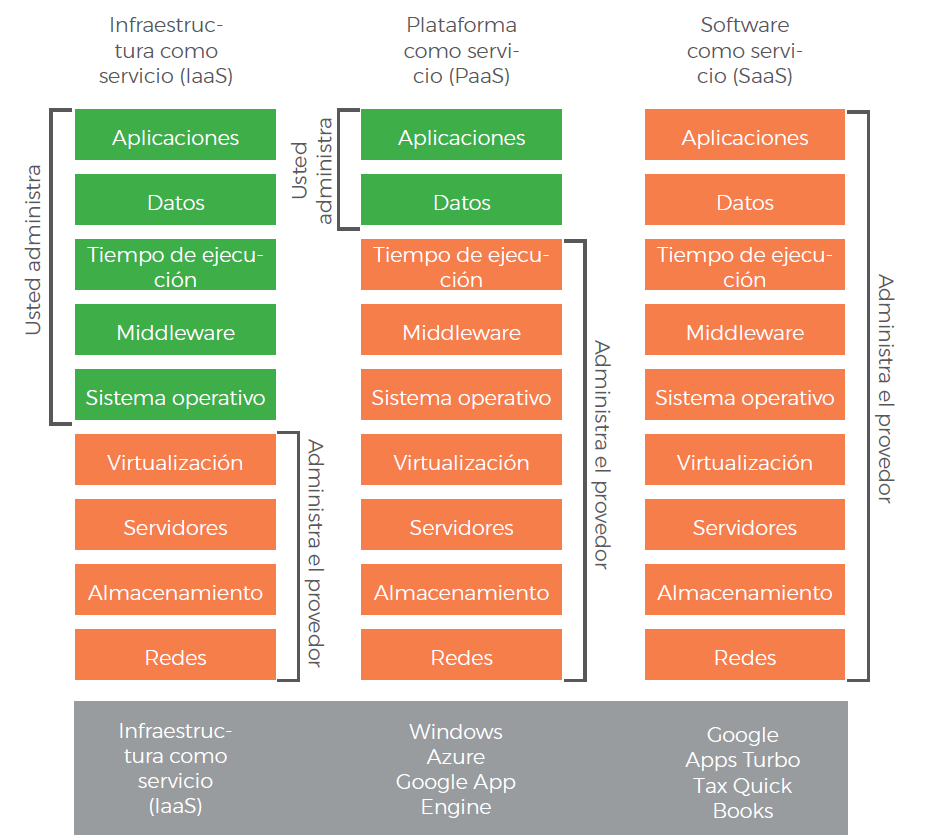
\includegraphics[width=.8\textwidth]{./Figures/capas-servicios.png}
%	\caption{Infraestructura por capas según el servicio  \citep{BOOK:2}.}

%	\label{fig:capas-servicios}
%\end{figure}

%\footnotetext{Imagen tomada del libro \textit{Cloud Computing for Pymes}. \citep{BOOK:1}}}



\section{Protocolo MQTT}

MQTT  (\textit{Message Queue Telemetry Transport}) es un protocolo de red ligero de mensajería estándar para IoT. Está diseñado como un transporte de mensajería extremadamente liviano y se utiliza en una amplia variedad de industrias, como la automotriz, las telecomunicaciones, el petróleo y el gas, entre otros  \citep{WEBSITE:4}. 

Para construir una red usando MQTT es necesario entender los conceptos que se utilizan para crear una red IoT: 

\begin{itemize}
\item El broker MQTT: el servidor o broker es el programa que se encarga de recepcionar los mensajes enviados por los clientes y distribuirlos entre sí en un sistema publicador-suscriptor. Los clientes envían periódicamente paquetes y esperan la respuesta del broker, como se ilustra con la figura \ref{fig:broker}. 

El broker MQTT usado en el trabajo es Eclipse Mosquitto, por ser de código abierto.

\begin{figure}[htbp]
	\centering
	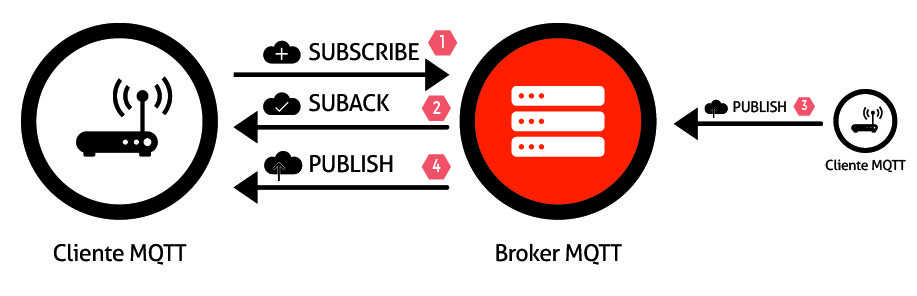
\includegraphics[width=.75\textwidth]{./Figures/broker.jpg}
	\caption{Funcionamiento del broker MQTT \protect\footnotemark..}
	\label{fig:broker}
\end{figure}
\footnotetext{Imagen tomada de \url{https://www.factor.mx/portal/base-de-conocimiento/mqtt/}}

%\vspace{1cm}
\item Comunicación MQTT: es la función de transporte de mensajes entre dispositivos IoT. El protocolo generalmente se ejecuta sobre TCP / IP ; sin embargo, cualquier protocolo de red que proporcione conexiones bidireccionales ordenadas y sin pérdidas puede admitir MQTT. Está diseñado para conexiones con ubicaciones remotas donde existen restricciones de recursos o el ancho de banda de la red es limitado \citep{WEBSITE:3}. Su modelo de comunicación se puede ver en la figura \ref{fig:mqtt}.

%\vspace{0.5cm}



La comunicación MQTT puede estar cifrada mediante TLS (\emph{Transport Layer Security}) y contar con credenciales de acceso para el control de los canales de envío y recepción. Al broker se le puede conectar un sinfín de dispositivos como teléfonos móviles, computadoras, sensores, actuadores, lámparas, relojes, bombas de agua, refrigeradores, cocinas y mucho más. 

\begin{figure}[htbp]
	\centering
	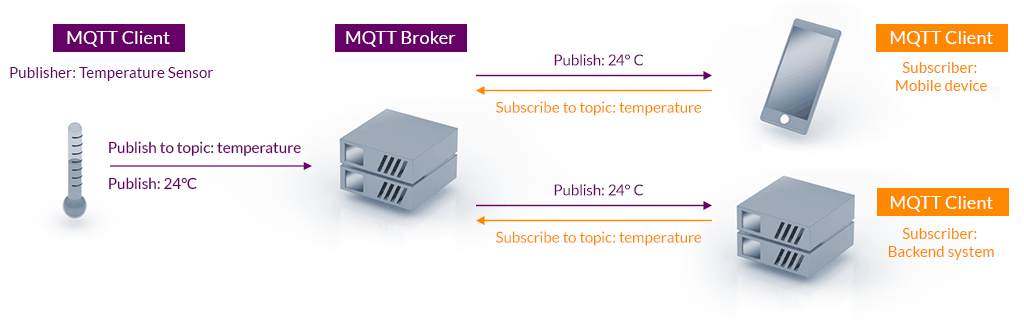
\includegraphics[width=0.95\textwidth]{./Figures/mqtt.png}
	\caption{Ejemplo de funcionamiento del protocolo MQTT \protect\footnotemark.}
	\label{fig:mqtt}
\end{figure}

\footnotetext{Imagen tomada de \url{https://mqtt.org/}}

\end{itemize}

%\section{Elementos del broker MQTT}


%\begin{itemize}
%\item Cliente: un dispositivo que puede publicar mensajes, suscribirse para recibir mensajes, o ambos.
%\item Broker: es el servidor que acepta mensajes publicados por clientes y los difunde entre los clientes suscritos.
%\item Publicar: cuando un cliente envía un mensaje al broker usando un tópico.
%\item Tópico: los mensajes deben estar etiquetados con algún tópico o tema. Los clientes se suscriben a tópicos específicos, de manera que solo reciben los mensajes publicados con dichos tópicos. 
%\end{itemize}


\section{Eclipse Mosquitto} 
Es un agente de mensajes de código abierto (con licencia EPL / EDL) cuya versión 2.0.14 implementa las versiones 5.0, 3.1.1 y 3.1 del protocolo MQTT. Mosquitto es liviano y adecuado para su uso en todos los dispositivos, desde computadoras de placa única de baja potencia hasta servidores completos \citep{WEBSITE:5}.

%El protocolo MQTT proporciona un método ligero para realizar mensajes mediante un modelo de publicación / suscripción. Esto lo hace adecuado para la mensajería de Internet de las cosas, como con sensores de baja potencia o dispositivos móviles como teléfonos, computadoras integradas o microcontroladores \citep{WEBSITE:5}.

Mosquitto es parte de la Fundación Eclipse \citep{WEBSITE:5}, es un proyecto de IoT \citep{WEBSITE:39} y está patrocinado por la compañía Cedalo \citep{WEBSITE:40}. 

\section{Componentes del módulo principal} 

El hardware del módulo principal integra la placa raspberry Pi 4 modelo B de 8 GB como placa base. La Raspberry Pi es una serie de ordenador de placa reducida, ordenador de placa única u ordenador de placa simple (SBC) de bajo costo desarrollado en el Reino Unido por la Raspberry Pi Foundation \citep{WEBSITE:6}.

La placa Raspberry Pi 4 es una pequeña computadora de escritorio de doble pantalla con opciones de salida en 4K, se puede usar como cerebro de robot, centro de hogar inteligente, centro multimedia, núcleo de IA (inteligencia artificial) en red y mucho más. La figura \ref{fig:rpi4} muestra sus principales especificaciones.

Las especificaciones técnicas de la computadora Raspberry Pi 4 son \citep{WEBSITE:7}:

\begin{itemize}
\item Broadcom BCM2711, SoC de 64 bits Cortex-A72 de cuatro núcleos (ARM V8) a 1,5 GHz.
\item SDRAM LPDDR4-3200 de 2 GB, 4 GB u 8 GB (según el modelo).
\item 2,4 GHz y 5,0 GHz IEEE 802.11ac inalámbrica, Bluetooth 5.0.
\item Gigabit Ethernet, 2 puertos USB 3.0 y 2 puertos USB 2.0.
\item Cabecera GPIO estándar Raspberry Pi de 40 pines (totalmente compatible con las placas anteriores).
\item Puertos micro-HDMI (hasta 4kp 60 compatible).
\item Ranura para tarjeta microSD para cargar el sistema operativo y el almacenamiento de datos.
\item 5 VCC a través del conector USB-C (mínimo 3 A).
\item 5 VCC a través del encabezado GPIO (mínimo 3 A).
\item Power over Ethernet (PoE) habilitado (requiere PoE HAT separado).
\item Temperatura de funcionamiento ambiente: 0 °C - 50 °C.
\end{itemize}

%%%%%%%%%%%%%%%%%%%%%%%%%%%%%%%%%%%%%%%%%%%%%%%%%%%%%%%%%%%%%%%%%%%
\begin{figure}[htbp]
	\centering
	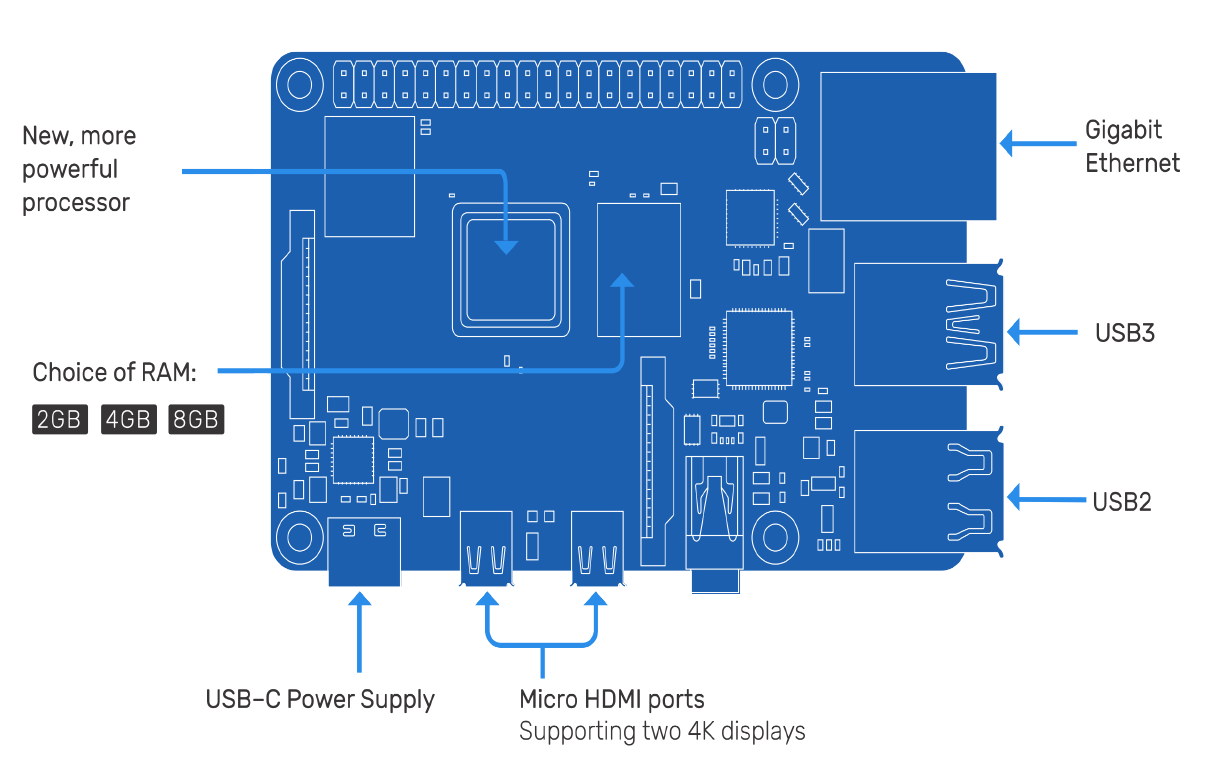
\includegraphics[width=1.0\textwidth]{./Figures/rpi4.png}
	\caption{Computadora Raspberry Pi 4 \protect\footnotemark. \citep{WEBSITE:7}}

	\label{fig:rpi4}
\end{figure}

\footnotetext{Imagen de \url{https://www.raspberrypi.com/products/raspberry-pi-4-model-b/specifications/}}

%\vspace{1cm}

%%%%%%%%%%%%%%%%%%%%%%%%%%%%%%%%%%%%%%%%%%%%%%%%
\subsection{Alimentación, gabinete y unidad de almacenamiento}

La fuente de alimentación para la Raspberry Pi 4 es de 3 A como se aprecia en la figura \ref{fig:placarpi4}. La unidad de almacenamiento contiene una unidad de memoria extraíble microSD de 64 GB y de clase 10 para garantizar alta velocidad de lectura y escritura durante el procesamiento.
% La figura \ref{fig:microsd} muestra la microSD del módulo.

\begin{figure}[htpb]
\centering 
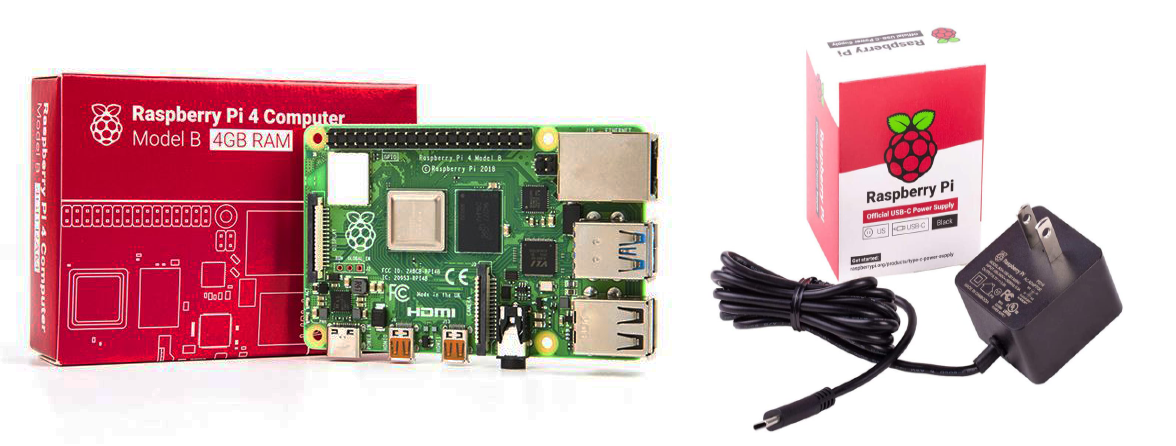
\includegraphics[width=0.8\textwidth]{./Figures/placa.png}
\caption{Mainboard y fuente de alimentación del servidor.}
\label{fig:placarpi4}
\end{figure}
%\begin{figure}[htpb]
%\centering 
%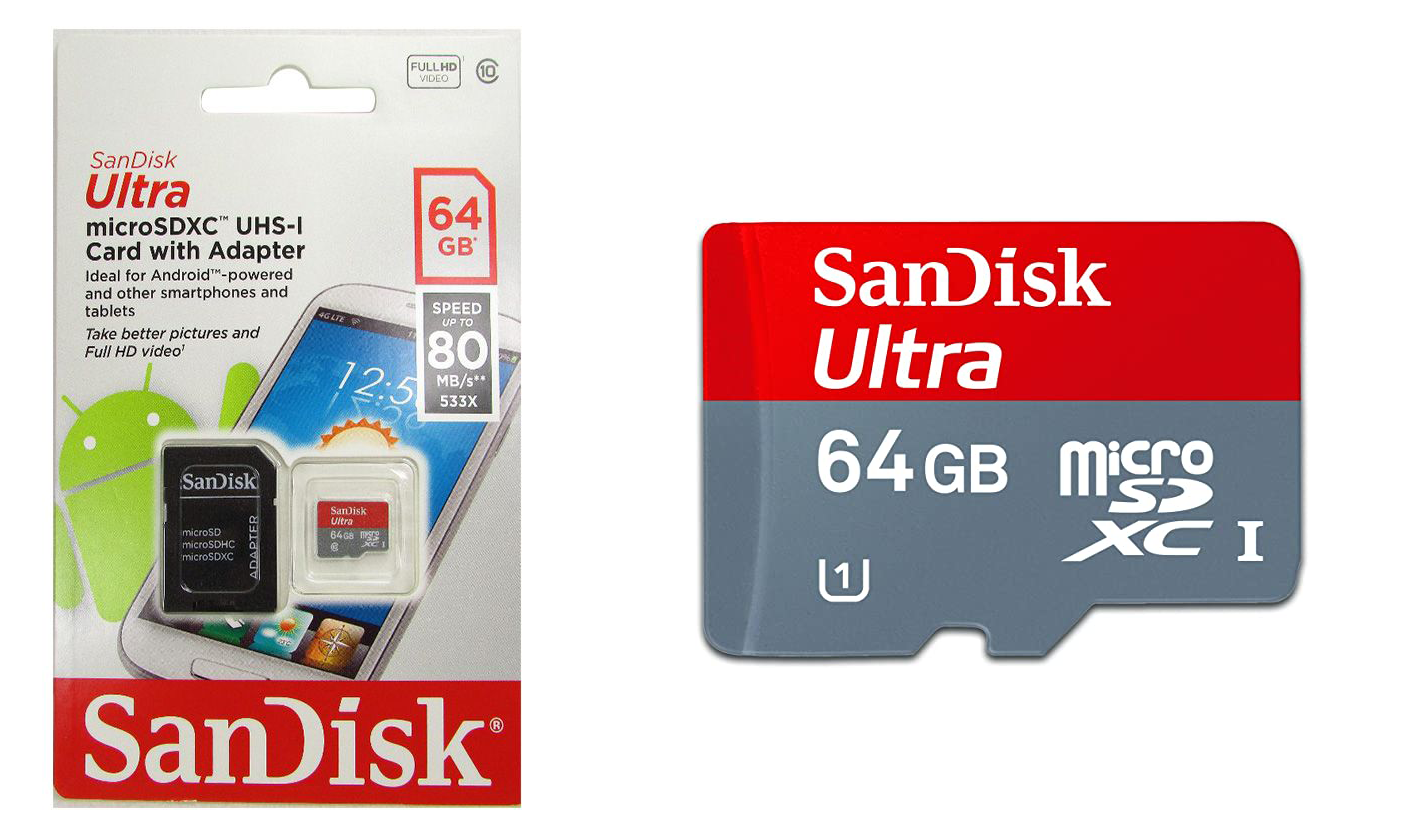
\includegraphics[width=0.7\textwidth]{./Figures/card.png}
%\caption{Tarjeta de almacenamiento del servidor local.}
%\label{fig:microsd}
%\end{figure}
El case Argon One Pi4 V2 es el gabinete usado para este trabajo como componente para la integración de elementos del módulo principal. La figura \ref{fig:armado} muestra las partes del gabinete.  
\vspace{0.5cm}

%Características del gabinete \citep{WEBSITE:16}:

%\begin{itemize}
%\item Tiene una placa Raspberry Pi Sata, que está diseñada para maximizar las transferencias de datos de alta velocidad para el uso de SSD Raspberry Pi 4; lo que la hace perfecta para el uso multimedia y otras aplicaciones. 
%\item La funda SSD Raspberry Pi solo es compatible con SSD M.2 SATA con llave B-Key o B+M.
%\item El SSD se conecta al Raspberry Pi 4 a través del puente USB en un puerto USB 3.0. 
%\item El case Argon incluye dos puertos HDMI de tamaño completo e IR integrado para la funcionalidad remota y también posee arranque automático. 
%\item El case Argon Raspberry Pi 4 tiene todos los pines GPIO accesibles en la parte superior de la funda mientras están protegidos por una cubierta magnética extraíble cuando no están en uso. 
%\item El case Argon ONE Raspberry Pi 4 obtiene la mejor experiencia de refrigeración gracias al \emph{software} Pi Fan \citep{WEBSITE:42} mientras que la funda actúa como un disipador de calor conectado a la CPU.
%\end{itemize}


\begin{figure}[htpb]
\centering 
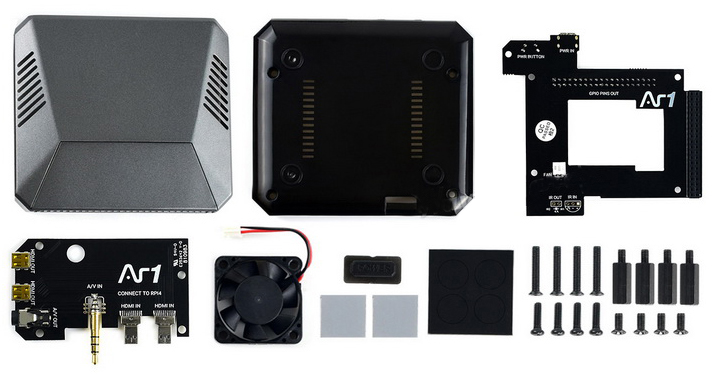
\includegraphics[width=1.0\textwidth]{./Figures/argon2.jpg}
\caption{Partes del gabinete Argon One Pi4 V2 \protect\footnotemark.}
\label{fig:armado}
\end{figure}
\footnotetext{Imagen tomada de \url{https://www.dfrobot.com/product-2090.html}}

\subsection{Sistema operativo para el servidor local}

En la actualidad existen mucha variedad de sistemas operativos para la placa Raspberry Pi, pero para este trabajo se usó el sistema operativo oficial y recomendado por la Raspberry Pi Foundation, llamado ``Raspberry Pi OS'' - version 11 basado en el kernel 5.15.

%La web oficial ofrece diversas versiones a las cuales se puede acceder con descarga directa como se ilustra con la figura \ref{fig:so}.

%\begin{figure}[htbp]
%	\centering
%	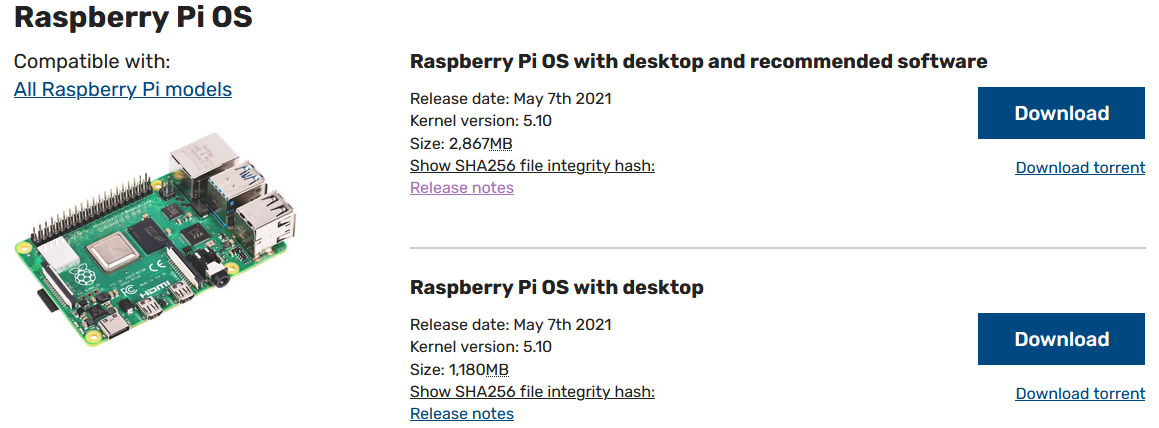
\includegraphics[width=1.0\textwidth]{./Figures/so.png}
%	\caption{Versiones del sistema operativo para Raspberry Pi \protect\footnotemark.}
%	\label{fig:so}
%\end{figure}
%\footnotetext{Imagen tomada de \url{https://www.raspberrypi.com/software/operating-systems/}}

\section{Hardware, sensores y actuadores}

Los componentes principales usados en el desarrollo de cada módulo están formados por una placa base NodeMCU, sensores y actuadores.

\subsection{Placa NodeMCU ESP8266}

La tarjeta NodeMCU es de bajo costo y está basada en el procesador ESP8266, que es muy utilizado en la realización de proyectos IoT, ya que dispone de Wi-Fi integrado. El procesador se programa en Lua \citep{WEBSITE:38}, pero también se puede programar con C/C++. Su principal característica es que trabaja a 3,3 V.  Además, ofrece más ventajas como la incorporación de un regulador de tensión integrado, así como un puerto USB de programación. 

%En el mercado actual se encuentran dos versiones muy utilizadas de la familia NodeMCU y la forma rápida de diferenciar la V2 de la V3, es fijarnos en el conversor serial que monta y en su tamaño. El CP2102 (V2) que es cuadrado, y el CH340G (V3) que es más alargado respectivamente,.
 
Para el trabajo se usó la placa versión 3 del NodeMCU ESP8266 que contiene el driver CH340G requerido para operar el circuito integrado con la interfaz USB. La placa se ilustra con la figura \ref{fig:nodemcu}:

\begin{figure}[htbp]
	\centering
	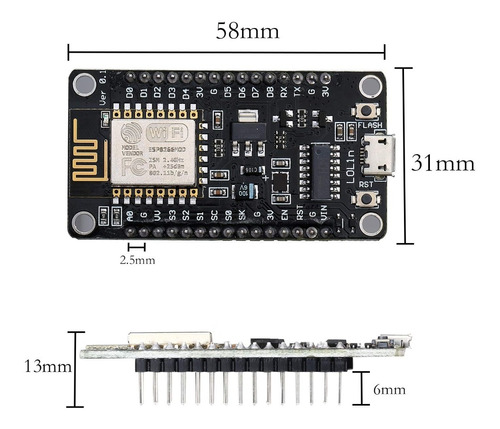
\includegraphics[width=.8\textwidth]{./Figures/nodemcuV3.jpg}
	\caption{Modelo y dimensiones de la placa NodeMCU ESP8266 V3.}

	\label{fig:nodemcu}
\end{figure}

\vspace{1.5 cm}
Las especificaciones técnicas del NodeMCU son:

\begin{itemize}
\item Utiliza chip CH340G (USB).
\item Tensión de alimentación: 4,5 V~9 V (10 V max) y/o alimentación por USB.
\item Tensión de pines I/O: 3,3 V.
\item Wireless 802.11 b/g/n standard.
\item Wi-Fi a 2,4 GHz, soporta encriptación WPA/WPA2.
\item Soporta tres modos de operación: STA/AP/STA+AP.
\item Pila de almacenamiento para protocolo TCP/IP (5 conexiones máximo).
\item Pines: D0~D8, SD1~SD3 pueden ser usados como GPIO, PWM, IIC con capacidad de drenar 15 mA por pin.
\item 1 canal ADC: AD0.
\item Consumo de corriente continua ≈ 70 mA (200 mA MAX), Standby: <200 uA.
\item Velocidad de transmisión: 110 - 460800 bps.
\item Soporta interfaz de comunicación UART/GPIO.
\item OTA: \emph{Remote firmware upgrade}.
\item Soporta \emph{Smart Link Smart Networking}.
\item Temperatura de trabajo: -40 ℃ - +125 ℃.
\item Memoria: 4 MByte.
\end{itemize}

\subsection{Sensor de temperatura y humedad DHT11}

El DHT11 es un sensor de humedad relativa y temperatura de media precisión de bajo costo. La salida suministrada es de tipo digital y utiliza solamente un pin de datos. Es usado en aplicaciones académicas relacionadas al control automático de temperatura, aire acondicionado, monitoreo ambiental en agricultura y más. El sensor se muestra en la figura \ref{fig:dht11}.

Utilizar el sensor DHT11 con las plataformas Arduino, Raspberry Pi y NodeMCU es muy sencillo tanto a nivel de \emph{firmware} como \emph{hardware}. A nivel de \emph{software} se dispone de bibliotecas para Arduino con soporte para el protocolo \emph{single bus}. En cuanto al hardware, solo es necesario conectar el pin VCC de alimentación a 3 V - 5 V, el pin GND a tierra y el pin de datos a un pin digital de Arduino \citep{WEBSITE:8}. 

\begin{figure}[htbp]
	\centering
	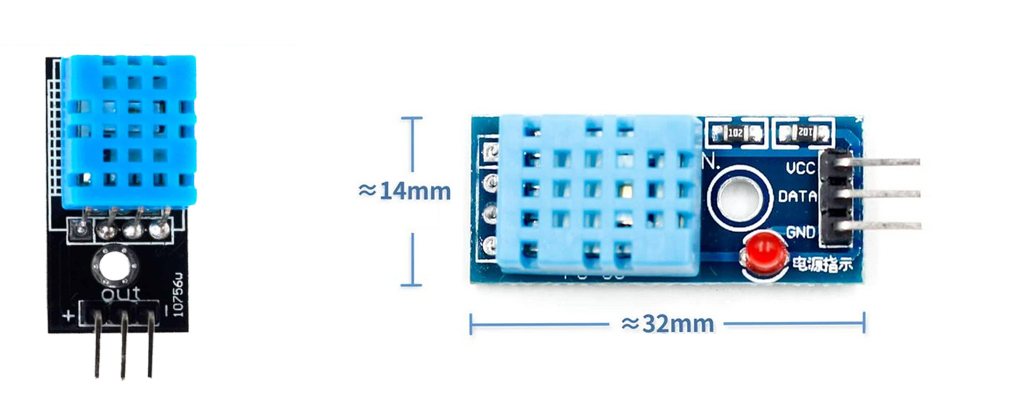
\includegraphics[width=.7\textwidth]{./Figures/dht11.jpg}
	\caption{Modelo y dimensiones del sensor DHT11. }

	\label{fig:dht11}
\end{figure}

Las características más importantes del sensor son:

\begin{itemize}
\item Tensión de operación: 3 V - 5 V DC.
\item Rango de medición de temperatura: 0 a 50 °C.
\item Precisión de medición de temperatura: ±2.0 °C.
\item Resolución temperatura: 0,1 °C.
\item Rango de medición de humedad: 20\% a 90\% RH.
\item Precisión de medición de humedad: 5\% RH.
\item Resolución humedad: 1\% RH
\item Tiempo de sensado: 1 seg.
\item Interface digital: \emph{Single-bus}.
\item Modelo: DHT11
\item Peso: 1 g.

\end{itemize}

\subsection{Sensor de corriente AC SCT-013-030}

La familia de sensores SCT-013 está compuesta por sensores de corriente no invasivo que permiten medir la intensidad que atraviesa un conductor sin necesidad de cortar o modificar el conductor. Estos sensores son usados para medir la intensidad o potencia consumida por una carga eléctrica. Los sensores SCT-013 son transformadores de corriente, dispositivos de instrumentación que hacen posible una medición proporcional a la intensidad que atraviesa un circuito. La medición se realiza por inducción electromagnética \citep{WEBSITE:9}. 

Los sensores SCT-013 disponen de un núcleo ferromagnético partido (como una pinza) que permite abrirlo para arrollar un conductor de una instalación eléctrica sin necesidad de cortarlo, como se ilustra con la figura \ref{fig:sensorCorriente}. Dentro de la familia SCT-013 existen modelos que proporcionan la medición como una salida de intensidad o de tensión. 


\begin{figure}[htbp]
	\centering
	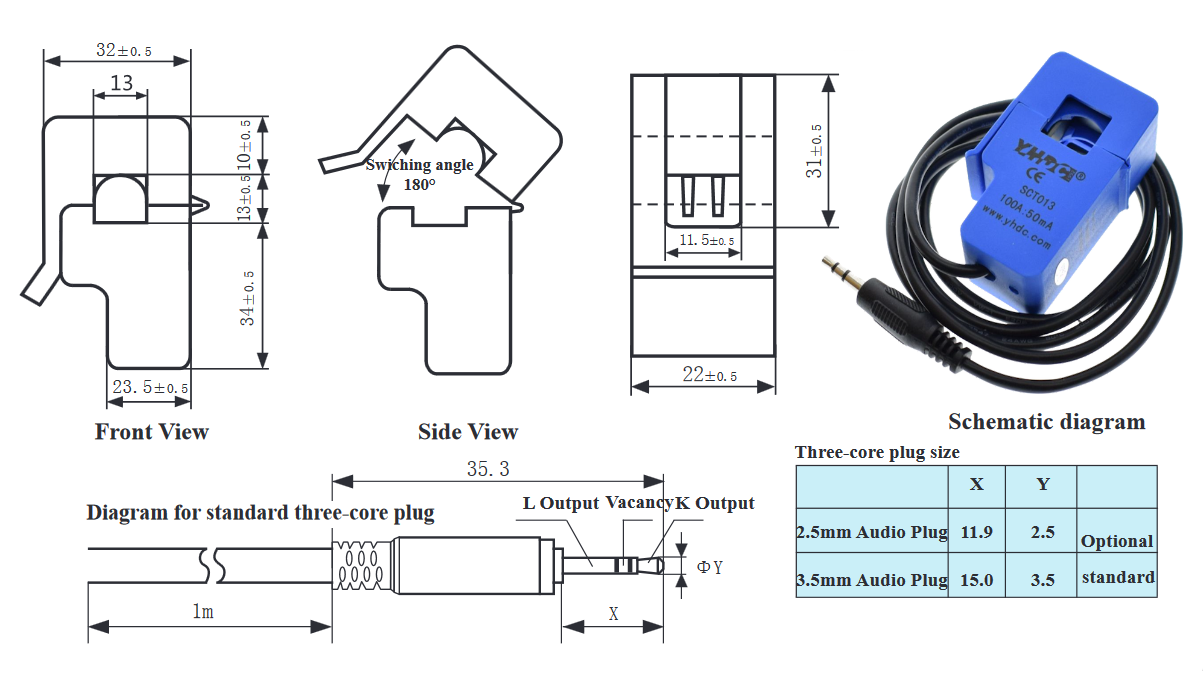
\includegraphics[width=1.0\textwidth]{./Figures/sensorCorriente2.png}
	\caption{Dimensiones del sensor SCT-013-030 AC \protect\footnotemark.}
	\label{fig:sensorCorriente}
\end{figure}

\footnotetext{Imagen de \url{https://datasheetspdf.com/pdf-file/1004704/XiDiTechnology/SCT-013-030/1}}

%El sensor SCT-013 es muy fácil de manejar y acoplar. Puede colocarse como una pinza alrededor de un cable que entre al edificio sin la necesidad de realizar algún trabajo de alta tensión, adecuado para la medición de corriente AC, monitoreo y protección de motores AC, equipo de iluminación, etc \citep{WEBSITE:10}.

Los sensores de la serie SCT-013 son sensores que trabajan como transformadores, la corriente que circula por el cable que se desea medir actúa como el devanado primario (1 espira) e internamente tiene un devanado secundario que dependiendo del modelo puede tener hasta más de 2000 espiras. La cantidad de espiras representa la relación entre corriente que circula por el cable y la que el sensor entrega. Esta relación o proporción es lo que marca la diferencia entre los diferentes modelos SCT-013, adicionalmente pueden tener una resistencia de carga en la salida y de esta forma en lugar de corriente se trabaja con una salida de tensión \citep{WEBSITE:21}. La figura \ref{fig:espiras} ilustra los devanados mencionados:

\begin{figure}[htpb]
\centering 
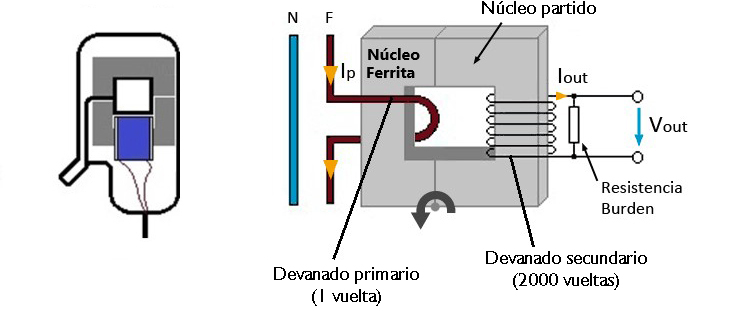
\includegraphics[width=1.0\textwidth]{./Figures/espiras.jpg}
\caption{Partes del núcleo ferromagnético del sensor de corriente.}
\label{fig:espiras}
\end{figure}

Las especificaciones más importantes por las cuales se escogió este instrumento para el desarrollo del trabajo son:

\begin{itemize}
\item Corriente de entrada (inducción): 0-30 A AC.
\item Modo de salida: 0 - 1 V.
\item No linealidad: ±1%.
\item Resistencia (RL): 62 $\Omega $.
\item Grado de Resistencia: Grade B.
\item Temperatura de operación: -25 °C - ﹢70 °C.
\item Longitud del cable: 1 m.
\item Tamaño abierto: 13 mm x 13 mm.
\end{itemize}

%La precisión del sensor puede ser del 1\% a 2\%, pero para ello es muy importante que el núcleo ferromagnético se cierre adecuadamente. Hasta un pequeño hueco de aire puede introducir desviaciones del 10\%. Como desventaja, al ser una carga inductiva, el SCT-013 introduce una variación del ángulo de fase cuyo valor es función de la carga que lo atraviesa, pudiendo llegar a ser de hasta 3º \citep{WEBSITE:9}.

%Los sensores SCT-013 son pequeños transformadores de corriente o CT (\emph{Current transformartor}) instrumentos ampliamente empleados como elementos de medición. Un transformador de corriente es similar a un transformador de tensión y está basado en los mismos principios de funcionamiento. Sin embargo, persiguen objetivos diferentes \citep{WEBSITE:9}.



%La relación de transformación de intensidad se expresa entre el número de espiras, como se muestra en ecuación \ref{eq:proporcionform}.

%\begin{equation}
%	\label{eq:proporcionform}
%	\left( \frac{Is}{Ip} \right)=\left( \frac{Vp}{Vs} \right)=\left( \frac{Np}{Ns} \right)
%\end{equation}

%A esto se le llama relación de transformación. Relaciona el número de espiras del devanado primario (Np), del devanado secundario (Ns), las intensidades del primario (Ip), del secundario (Is), la tensión del primario (Vp) y del secundario (Vs). 


%Para utilizar el sensor SCT-013 no es necesario interrumpir (cortar o desempalmar) el cable a medir, porque al igual que una pinza amperimétrica tiene el núcleo partido. Si se pasa los dos cables de una conexión monofásica, la lectura será 0, puesto que los cables tienen corrientes opuestas \citep{WEBSITE:21}. La figura \ref{fig:conectacorrecto} ilustra la forma correcta de uso del sensor.

%\vspace{0.5cm}
%\begin{figure}[htpb]
%\centering 
%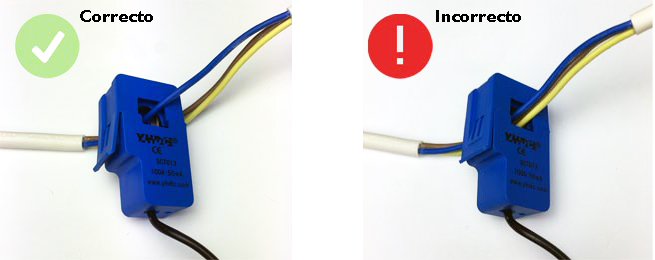
\includegraphics[width=0.8\textwidth]{./Figures/correcto.jpg}
%\caption{Forma de uso del sensor de corriente \protect\footnotemark.}
%\label{fig:conectacorrecto}
%\end{figure}

%\footnotetext{Imagen de \url{https://programarfacil.com/blog/arduino-blog/sct-013-consumo-electrico-arduino/}}


A diferencia de los transformadores de tensión, en un transformador de intensidad el circuito secundario nunca debe estar abierto, porque las corrientes inducidas pueden llegar a dañar el componente. Por este motivo, los sensores SCT-013 disponen de protecciones (resistencia de Burden en los sensores de salida por tensión, o diodos de protección en los sensores de salida por corriente)\citep{WEBSITE:9}.

Para el trabajo se consideró el módulo SCT-013 de 30 A y con soporte para 250 VAC.
%%%%%%%%%%%%%%%%%%%%%%%%%%%%%%%%%%%%%%%%%%%%
\subsection{Sensor de tensión eléctrica AC - ZMPT101B}

El sensor transformador de tensión ZMPT101B permite medir tensión alterna como la que se dispone en la red hogareña. Esta tensión AC no puede ser medida directamente por el ADC del circuito o placa debido a que escapa del rango de entrada (0 V a 5 V). El módulo ZMPT101B soluciona el problema reduciendo la tensión AC de entrada a una tensión menor que pueda ser leída por el Arduino, NodeMCU o cualquier otro microcontrolador. La figura \ref{fig:sensortension} ilustra la forma de conexión del módulo sensor a la línea eléctrica doméstica.

El sensor está integrado por un transformador que cumple la función de aislador galvánico para mayor seguridad en el uso. El lado primario del transformador se conecta a la tensión alterna que se desea medir, por ejemplo la red eléctrica de un hogar de 220 VAC. En el lado secundario del transformador se encuentra un divisor de tensión y un circuito con amplificador operacional (OPAMP LM358) para adicionar un desplazamiento (\emph{offset}) a la salida análoga \citep{WEBSITE:22}. 

\begin{figure}[htpb]
\centering 
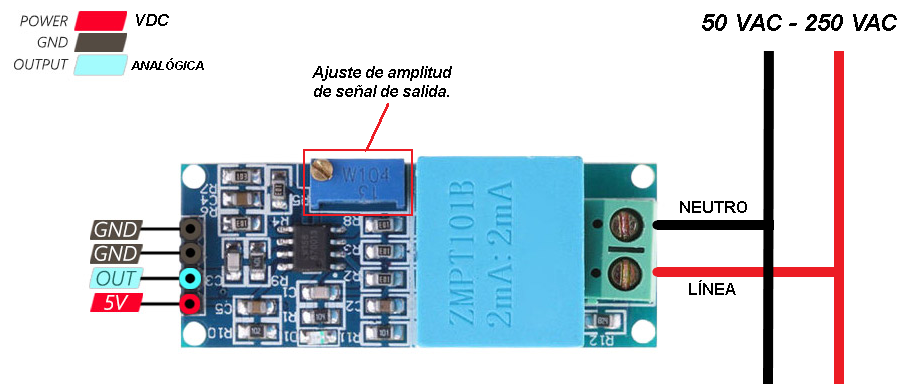
\includegraphics[width=0.95\textwidth]{./Figures/sensortension.png}
\caption{Conexión y partes del sensor de tensión.}
\label{fig:sensortension}
\end{figure}


Este sensor soporta una tensión de entrada de hasta 250 VAC y entrega una onda senoidal de amplitud regulable por un potenciómetro en placa. La onda senoidal de salida está desplazada positivamente para que no tenga tensiones negativas y así poder leerla completamente con el ADC. El desplazamiento depende de la tensión con la que se alimenta el módulo sensor: si la tensión de alimentación es de 5 V el desplazamiento será de 2,5 V y si se alimenta el módulo con 3,3 V el desplazamiento será de 1,65 V \citep{WEBSITE:23}. Su circuito de acondicionamiento de señal interno permite que la tensión de salida del módulo sensor pueda ser leído por cualquier microcontrolador con entrada analógica (ADC). De esta forma, es posible leer la tensión instantánea y realizar cálculos de energía como tensión pico a pico (Vpp) y tensión eficaz (Vrms). 

%Debido a la naturaleza de los transformadores, solo puede medir tensión AC \citep{WEBSITE:22} \citep{ARTICLE:1}. Para su uso con la tarjeta NodeMCU ESP8266, los extremos son 0 y 3.3 V con una compensación de 1.65 V. La figura \ref{fig:ondas} muestra el desplazamiento de onda senoidal.


%\begin{figure}[htpb]
%\centering 
%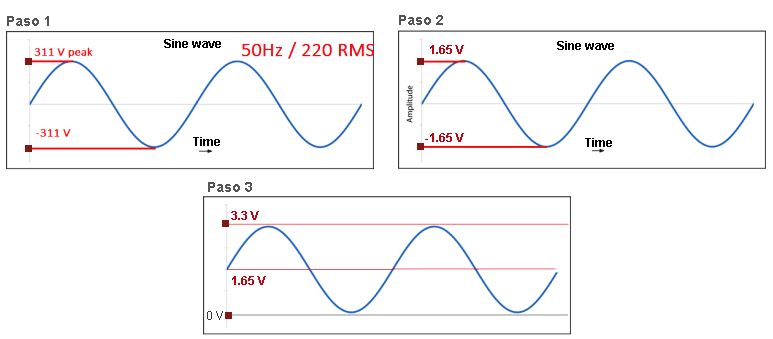
\includegraphics[width=1.02\textwidth]{./Figures/ondas.png}
%\caption{Señal del ZMPT101B con el NodeMCU ESP8266 \protect\footnotemark.}
%\label{fig:ondas}
%\end{figure}

%\footnotetext{Imagen tomada de \url{https://surtrtech.com/2020/04/08/}}

%%%%%%%%%%%%%%%%%%%%%%%%%%%%%%%%%%%%%%%%%%%%



\subsection{Relé Actuador}

Un relé es un interruptor que se puede activar mediante una señal eléctrica. En su versión más simple es un pequeño electro-imán que cuando se lo excita mueve la posición de un contacto eléctrico de conectado a desconectado o viceversa para accionar un circuito mayor. 

Los relés más utilizados son módulos capaces de activarse mediante la entrada de 5 V. La elección de un módulo relé adecuado dependerá de la tensión y amperaje que debe gestionar. En la figura \ref{fig:rele} se aprecian dos modelos de módulos relé con capacidad de activación 5 V y con soporte para 10 A - 250 VAC y 30 A – 250 VAC respectivamente.


\begin{figure}[htbp]
	\centering
	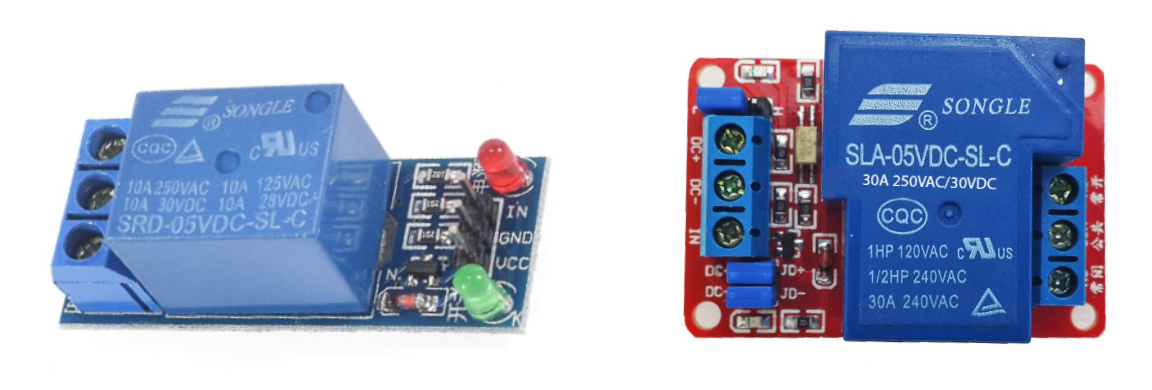
\includegraphics[width=1.0\textwidth]{./Figures/rele.jpg}
	\caption{Modelos de relés con activación de 5 V.}

	\label{fig:rele}
\end{figure}

%El relé es un interruptor que permite trabajar con dos circuitos, uno con tensiones elevadas, por ejemplo, 220 V pero que es activado por un circuito de tensión inferior, por ejemplo, 5 V.

Para el trabajo se consideró el módulo relé de activación 5 V y con soporte para 30 A - 250 VAC.

\subsection{Lenguajes de programación}

La elaboración de este trabajo involucró el usó de distintos \emph{software}s como herramientas para facilitar el desarrollo, así como el uso de diversos lenguajes de programación que se describen a continuación:
\begin{itemize}
\item Python: es un lenguaje de programación interpretado cuya filosofía hace hincapié en la legibilidad de su código. Se trata de un lenguaje de programación multiparadigma, ya que soporta parcialmente la orientación a objetos, programación imperativa y, en menor medida, programación funcional.

Se utilizó para la creación de procesos internos en el módulo principal. 
\item PHP: es un lenguaje de programación de uso general que se adapta especialmente al desarrollo web del lado del servidor.

Se utilizó como lenguaje \emph{backend} del \emph{software} de monitoreo y control.
\item JavaScript: lenguaje de programación interpretado utilizado en el lado del cliente. Es el único lenguaje de programación que funciona en los navegadores de forma nativa.

Se utilizó como lenguaje frontend del \emph{software} de monitoreo y control.
\item Arduino: lenguaje de programación que está basado en C++.

Se utilizó como lenguaje para programar el firmware de los módulos de sensores y actuadores.
\end{itemize} 
\chapter{Diseño e implementación} % Main chapter title

\label{Chapter3} % Change X to a consecutive number; for referencing this chapter elsewhere, use \ref{ChapterX}

En este capítulo se detallan las consideraciones de diseño que se tuvieron en cuenta para realizar el sistema IoT y se describe el desarrollo y servicios implementados para este trabajo.



%----------------------------------------------------------------------------------------
%	SECTION 1
%----------------------------------------------------------------------------------------


\section{Diseño general del sistema}

Como se observa en la \ref{fig:arquitectura}, el sistema está compuesto por una arquitectura que integra cuatro componentes necesarios para su funcionamiento, los dispositivos (sensores y actuadores), el servidor local, los elementos de red y el servicio en la nube.

El diseño del sistema se basó en una arquitectura distribuida donde se despliegan distintas tecnologías, \emph{hardware} y \emph{software} con el objetivo de ofrecer acceso local y remoto desde dentro o fuera de la red doméstica del edificio. Además, la interfaz de comunicación con el servidor interno y externo se hizo mediante el protocolo MQTT por ser ligero y de bajo consumo de ancho de banda de la red \emph{wireless} usada. 

El diseño del sistema comenzó con la modelización de los componentes más importantes del sistema IoT, que son los módulos, sensores y actuadores para posteriormente desarrollar el software de monitoreo de tipo web, usando los patrones y características de desarrollo web seguro. 

Como se eligió el protocolo MQTT para la comunicación entre módulos y el conjunto de servicios, se definió tres tipos de tópicos para poder comunicarse entre sí. Estos tópicos fueron:

\begin{itemize}
\item Tópicos para sincronización: permite que un módulo envié un dato JSON con los datos que deben actualizarse a todos los clientes suscritos a este tópico. Solo lo usan los módulos actuadores y el servidor local para la comunicación bidireccional.

\item Tópicos para envió de valores: permite que un módulo envié un dato JSON con valores de su sensor hacia el servidor. Es usado por sensores de comunicación unidireccional.

\item Tópicos para comunicación de estados: es usado por todos los módulos y permite el envió de un dato JSON con valores con su estado actual hacia sensor hacia el servidor. Es usado solo en comunicación unidireccional.
\end{itemize}

%\vspace{1cm}

%%%%%%%%%%%%%%%%%%%%%%%%%%% imagen horizontal%%%%%%%%%%%%%%%%%%%%%%%%%%%%%%%%%%%%%%%%%%%%
\begin{landscape} % esto es para rotar la pagina e imagen
\begin{figure}[htpb]
\centering 
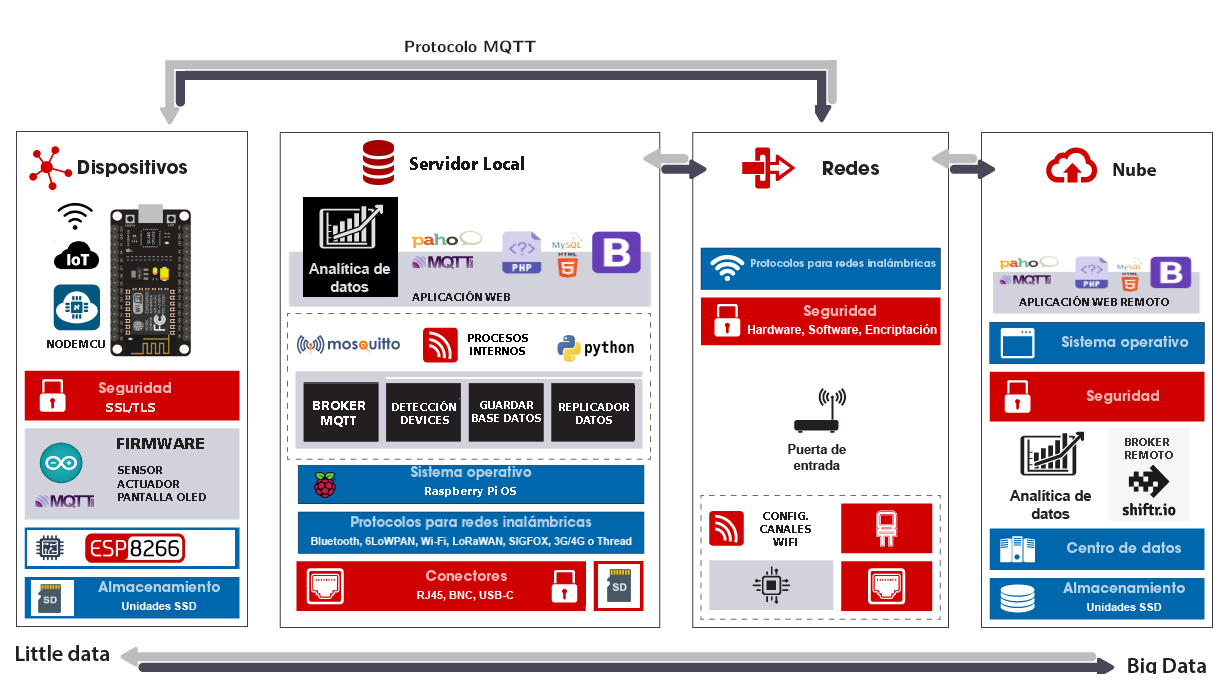
\includegraphics[width=1.65\textwidth]{./Figures/arquitectura-listo.png}
\caption{Arquitectura del sistema IoT.}
\label{fig:arquitectura}
\end{figure}
\end{landscape} % esto es para rotar
%%%%%%%%%%%%%%%%%%%%%%%%%%%%%%%%%%%%%%%%%%%%%%%%%%%%%%%%%%%%%%%%%%%%%%%%%%


El software de monitoreo del tipo web local y remoto fue diseñado y desarrollado a medida para garantizar dominio total de la plataforma usada. Utiliza el \emph{framework bootstrap} para lograr interfaces graficas de usuario que cumplan con los principios de experiencia de usuario (UX) y compatibilidad de dispositivos. Para la recepción de mensajes se usó web sockets mediante \emph{JavaScript} teniendo configurado los tres tópicos de comunicación antes mencionados para el intercambio de mensajes con los módulos.

La figura \ref{fig:diagrama_general} muestra el diagrama general del funcionamiento del sistema desde la perspectiva conceptual. El desarrollo, consideraciones de construcción y fabricación para cada módulo del sistema se describen a detalle en las siguientes secciones de este capítulo.


\begin{figure}[htbp]
	\centering
	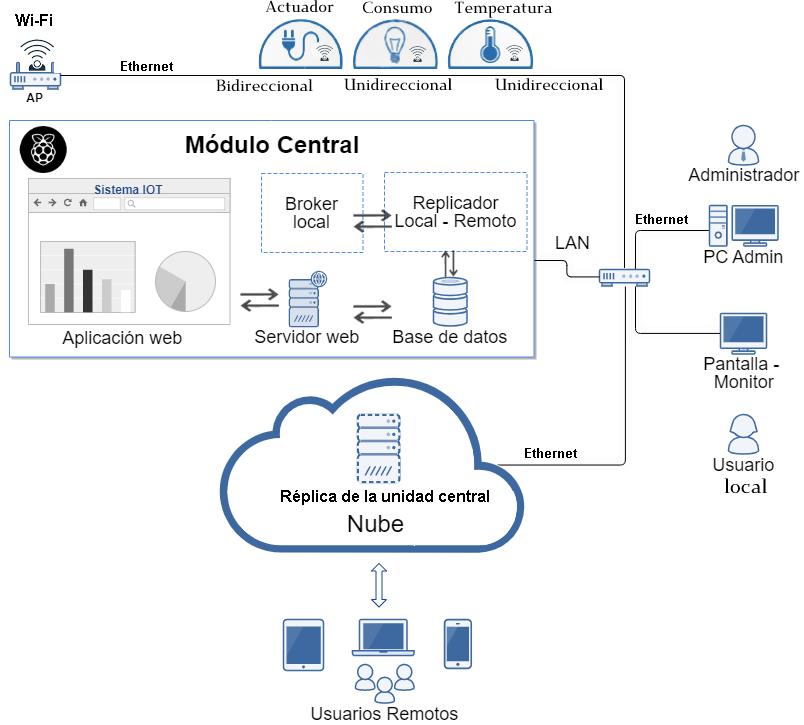
\includegraphics[width=0.9\textwidth]{./Figures/diagrama0.png}
	\caption{Diagrama general del funcionamiento del sistema.}

	\label{fig:diagrama_general}
\end{figure}

%\vspace{0.5cm}


%\section{Medidas de ciberseguridad}

%Los requerimientos de ciberseguridad dentro del desarrollo ocupan un lugar muy importante en cada una de las etapas ejecutadas en el proceso de implementación de un sistema IoT, porque permite garantizar un grado mínimo de seguridad y confiabilidad funcional del producto. 

%Los requerimientos considerados durante el proceso, son los siguientes:





%\subsection{Requerimientos para los módulos IoT}
%Se buscó cumplir con los requerimientos que se plantean a continuación:

%\begin{itemize}
%\item Uso de programación basada en código modular para el desarrollo del \emph{firmware}.
%\item Uso de la biblioteca en su versión más actual para la comunicación MQTT.
%\item Los objetos de datos a transmitir serán del formato JSON.
%\item La comunicación el protocolo MQTT debe contener TLS.
%\end{itemize}





%\section{Construcción y programación de módulos}

%En esta sección se describen el proceso y consideraciones técnicas para la construcción de cada uno de los módulos del sistema IoT propuesto.
%%%%%%%%%%%%%%%%%
\section{Módulo principal}

El módulo principal representa el elemento central dentro de la solución IoT planteada y para la construcción e instalación se utilizaron recursos que hicieron posible una versión de fácil uso para el usuario. Las consideraciones generales de seguridad para el módulo principal fueron:

\begin{itemize}
\item Sistema operativo GNU/Linux oficial Raspberry Pi OS.
\item Acceso al sistema operativo mediante usuario y contraseña.
\item Accesos remotos por SSH (\emph{Secure Shell}) y FTP (\emph{File Transfer Protocol})  desactivados.
\item Cifrado de las unidades del sistema operativo.
\end{itemize}

La figura \ref{fig:argon} muestra la integración y ensamblado del módulo.

%%%%%%%%%%%%%%%%%%%%%%%%%%% imagen horizontal%%%%%%%%%%%%%%%%%%%%%%%%%%%%%%%%%%%%%%%%%%%%
%\begin{landscape} % esto es para rotar la pagina e imagen
\begin{figure}[htpb]
\centering 
%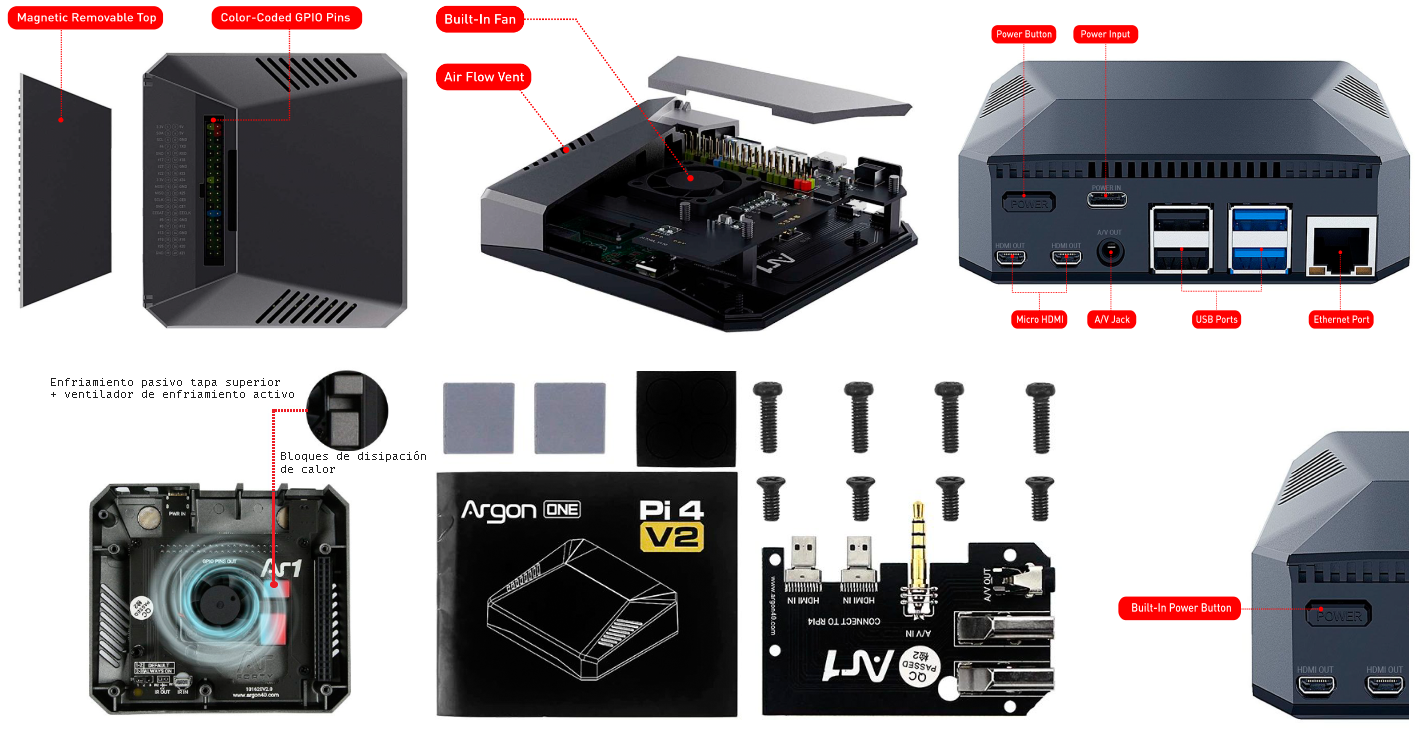
\includegraphics[width=1.7\textwidth]{./Figures/argon.png}
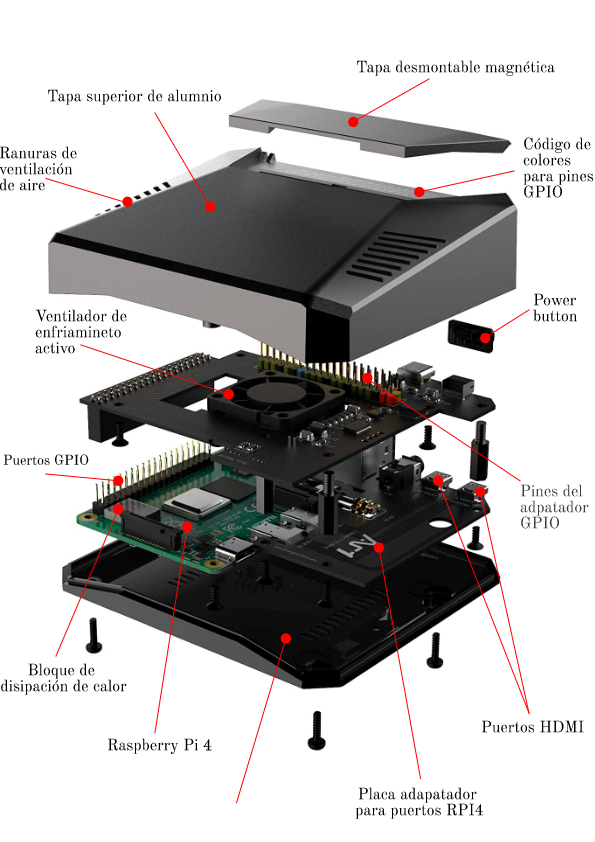
\includegraphics[width=0.92\textwidth]{./Figures/armadoactuador.png}
\caption{Ensamblado y partes del módulo principal. }
\label{fig:argon}
\end{figure}
%\end{landscape} % esto es para rotar
%%%%%%%%%%%%%%%%%%%%%%%%%%%%%%%%%%%%%%%%%%%%%%%%%%%%%%%%%%%%%%%%%%%%%%%%%%%





%Las consideraciones de seguridad para la configuración del broker fueron:

%\begin{itemize}
%\item Configuración de usuario y contraseña para controlar el acceso a los canales de comunicación del broker local y remoto.
%\item Uso de canales separados, para el envió, sincronización y respuesta entre elementos del sistema IoT.
%\item Cada mensaje debe ir con destino a un tópico en específico, evitar envió de datos a la instancia general \#.
%\item Configurar permisos para la edición o ejecución a los archivos de configuración del broker.
%\end{itemize}


\section{Módulo replicador a la nube}

El módulo replicador a la nube está dentro del módulo principal y para su desarrollo se diseñó una estructura interna compuesta por subprocesos que, al trabajar en conjunto, forman el sistema completo de replicación.

La replicación solo se da mientras exista conexión a Internet. El desarrollo de cada subproceso se programó en el lenguaje de programación Python por tratarse de un lenguaje multiplataforma, robusto y orientado a objetos. La figura \ref{fig:logicareplicador} ilustra la lógica de trabajo del replicador.


%\begin{figure}[htpb]
%\centering 
%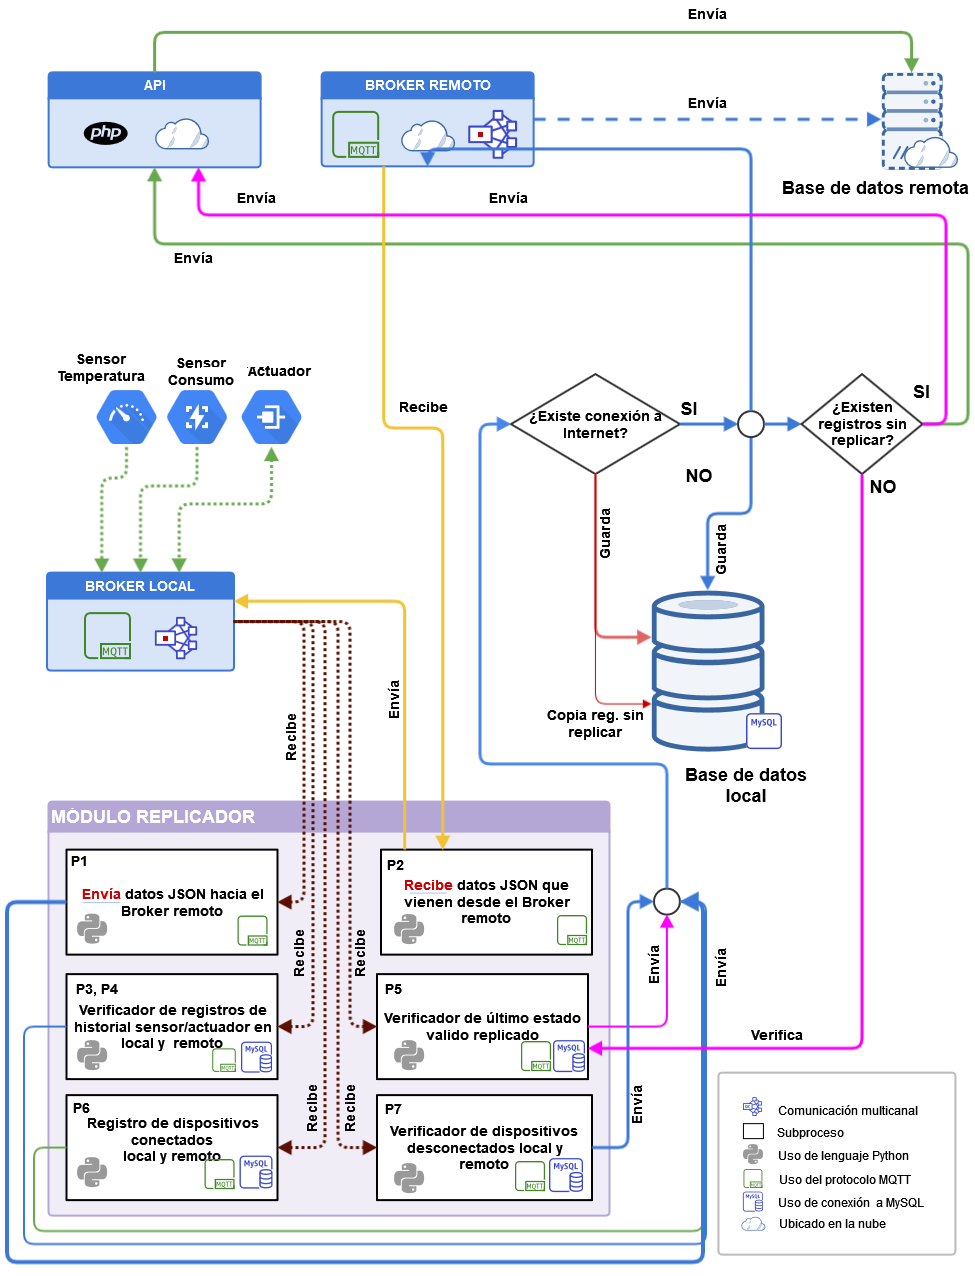
\includegraphics[width=1.15\textwidth]{./Figures/replicador.png}
%\caption{Flujo funcional del módulo replicador.}
%\label{fig:flujoreplicador}
%\end{figure}



Las descripciones de cada subproceso interno que contiene el módulo replicador, se detallan a continuación usando el nombre del proceso con el cual fue creado: 

\begin{itemize}
\item \keyword{mqtt\_envia\_nube\_poo (P1)}: es el responsable de enviar todos los datos que llegan de los canales hacia el broker remoto usando el formato JSON.

\item \keyword{mqtt\_recibe\_nube\_poo (P2)}: es el responsable de recibir los datos JSON que fueron generados en la aplicación web remota y que llegan desde el broker remoto para luego transmitirlo.

\item \keyword{actuador\_registros\_bd (P3)}: es el responsable de verificar los registros en la base de datos. Su verificación está basada en intervalos de tiempo de una hora, consulta todos los registros de lecturas de actuadores dentro de una hora específica en las tablas auxiliares de actuadores y consumos, luego obtiene la media de los consumos y hace un solo registro en la tabla de historial de consumo. Este subproceso realiza un borrado de registros temporales de las tablas auxiliares de actuadores por cada registro en la tabla historial.

\item \keyword{sensor\_registros\_bd (P4)}: es el responsable de verificar los registros en la base de datos. Su verificación está basada en intervalos de tiempo de una hora, consulta todos los registros de lecturas de sensores dentro de una hora específica en las tablas auxiliares de sensores, luego obtiene la media de los registros y hacer un solo registro en la tabla de historial de sensores. Este subproceso realiza un borrado de registros temporales de las tablas auxiliares de sensores por cada registro en la tabla historial.

\item \keyword{sensor\_historial\_replicas\_bd (P5)}: es el responsable de verificar de forma constante la conexión a Internet y si existen datos por replicar, en caso de disponer de una conexion a Internet y a partir de registros marcados como no replicados, este procederá a enviar los últimos registros hacia la nube, para luego actualizar en campo de la tabla de registros\_no\_enviados, y así mantener la consistencia necesaria para el sistema local y remoto.

\item \keyword{mqtt\_gestionBD\_poo (P6)}: es el responsable de recibir todos los mensajes que llegan al broker y verificar la pertenencia del JSON capturado (sensor o actuador), posteriormente, comprueba si existe conexión a Internet y poder registrar en la base de datos local y remoto. En caso que no existiera conexión a Internet, solo registra en la tabla correspondiente al sensor o actuador de la base de datos local y a su vez marca el registro como no replicado, para que pueda ser enviado a la nube cuando vuelva a existir la conexión a Internet. Este subproceso también permite actualizar el estado de un sensor o actuador en la base de datos con el estado de ``CONECTADO'' mientras esté activo en la red.

%\vspace{0.05cm}
%%%%%%%%%%%%%%%%%%%%%%%%%%% imagen horizontal%%%%%%%%%%%%%%%%%%%%%%%%%%%%%%%%%%%%%%%%%%%%
\begin{landscape} % esto es para rotar la pagina e imagen
\begin{figure}[htbp]
	\centering
	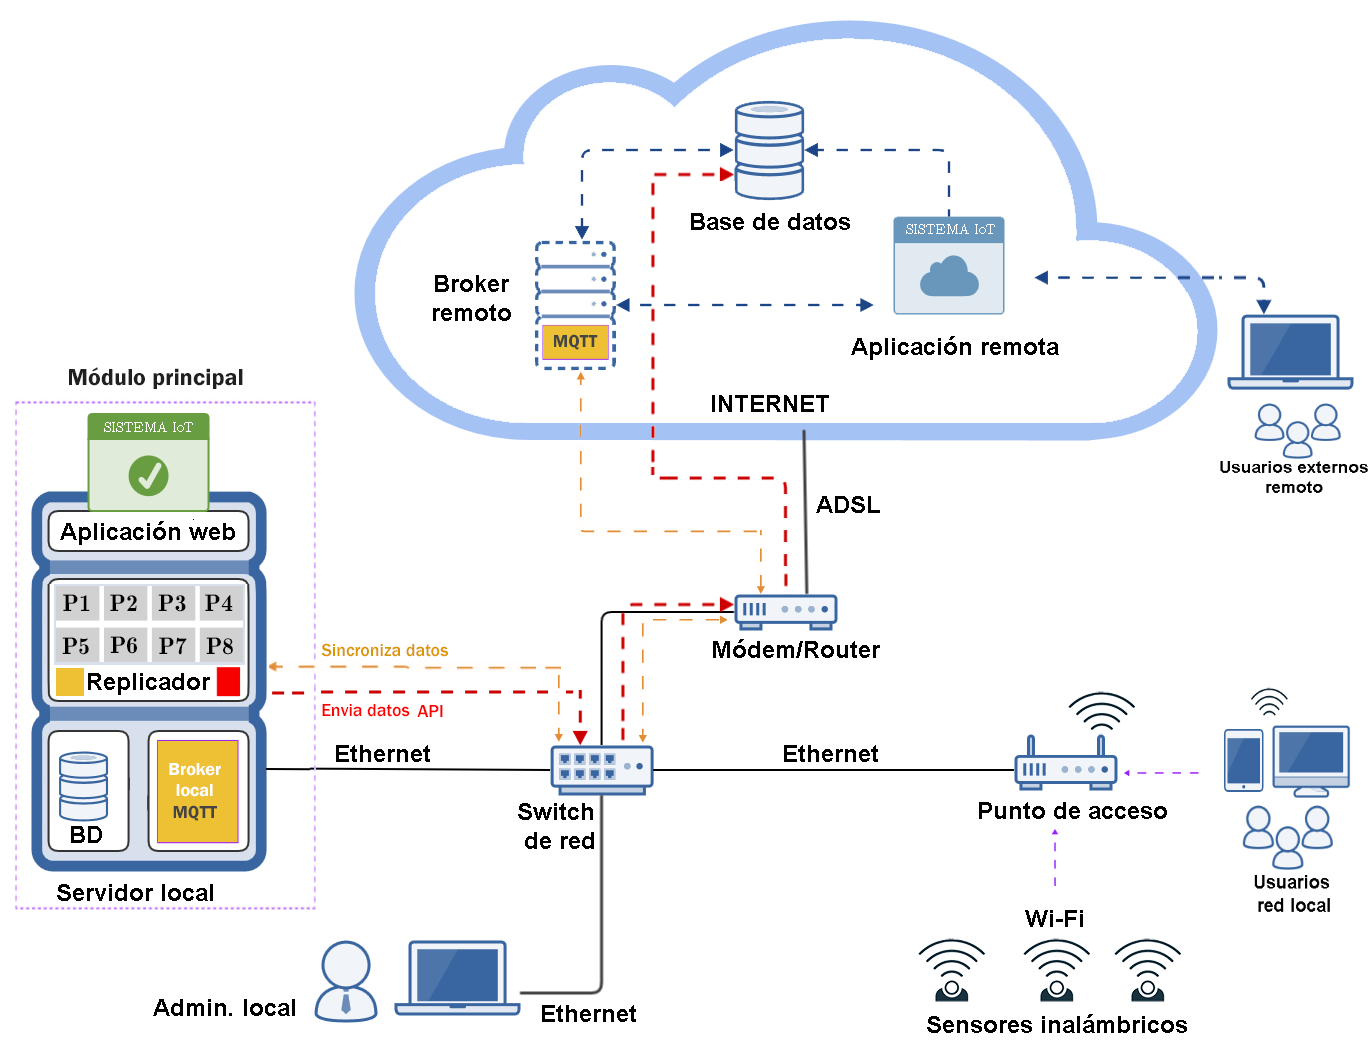
\includegraphics[width=1.2\textwidth]{./Figures/diagrama2.png}
	\caption{Diagrama funcional del replicador. }

	\label{fig:logicareplicador}
\end{figure}
\end{landscape} % esto es para rotar
%%%%%%%%%%%%%%%%%%%%%%%%%%%%%%%%%%%%%%%%%%%%%%%%%%%%%%%%%%%%%%%%%%%%%%%%%%%

\item \keyword{mqtt\_gestionDispositivosConectados (P7)}: es el responsable de recibir todos los mensajes que llegan al broker, verificar la pertenencia del JSON capturado (sensor o actuador) para registrar temporalmente el tiempo de llegada del mensaje del dispositivo. 

Este subproceso usa hilos en Python para estar constantemente registrando los tiempos de llegada de mensajes de cada sensor o actuador, y si los intervalos de tiempo de llegada de mensajes para un dispositivo activo son mayores a un minuto, el subpoceso actualiza el estado del dispositivo con el estado de ``DESCONECTADO'' en la base de datos.

\item \keyword{sensorEstadoRed (P8)}: es el responsable de verificar el estado del servicio de Internet en la red WLAN. Este subproceso usa hilos en Python para registrar periódicamente en la base de datos el estado actual de la red interna.

\end{itemize}

\section{Módulo de medición de temperatura}

Este módulo permite recoger lecturas del valor de la temperatura y humedad en ambientes de un hogar, oficina o edificio. Los valores son enviados y procesados en el sistema IoT de control y monitoreo que se encuentra en el servidor web del módulo principal. Las lecturas de temperatura son utilizadas para conocer la curva de cambios de temperatura según el horario registrado, así como su relación directa con el consumo eléctrico por el uso de ventiladores y equipos de aire acondicionado. Para su construcción se usó la placa NodeMCU8266 V3, por la capacidad de conexión inalámbrica. 

Este módulo integra una pantalla SSD1306 OLED para visualizar el valor de la temperatura en tiempo real. Para el encapsulado y construcción se utilizó un tablero adosable de montaje de interruptores térmicos y diferenciales tipo RIEL-DIN, de material de poliestireno y cubierta trasparente de policarbonato con apertura vertical \citep{WEBSITE:17}, como se aprecia en la figura \ref{fig:casetemp}.


\begin{figure}[htpb]
\centering 
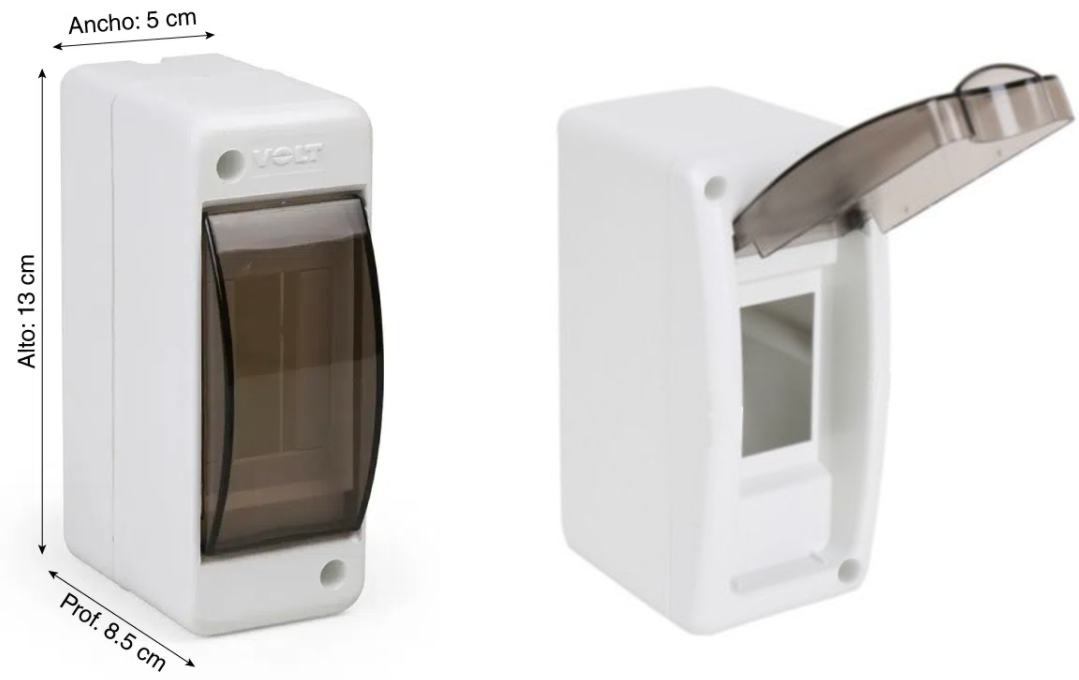
\includegraphics[width=0.7\textwidth]{./Figures/casetemp.png}
\caption{Case del módulo de temperatura \protect\footnotemark.}
\label{fig:casetemp}
\end{figure}

\footnotetext{Imagen tomada de \url{https://www.promart.pe/tablero-2-polos-adosable-c-puerta/p}}

El diseño de integración de componentes electrónicos se realizó en una Placa PCB perforada siguiendo el esquemático de la figura \ref{fig:citemp}.

\begin{figure}[htpb]
\centering 
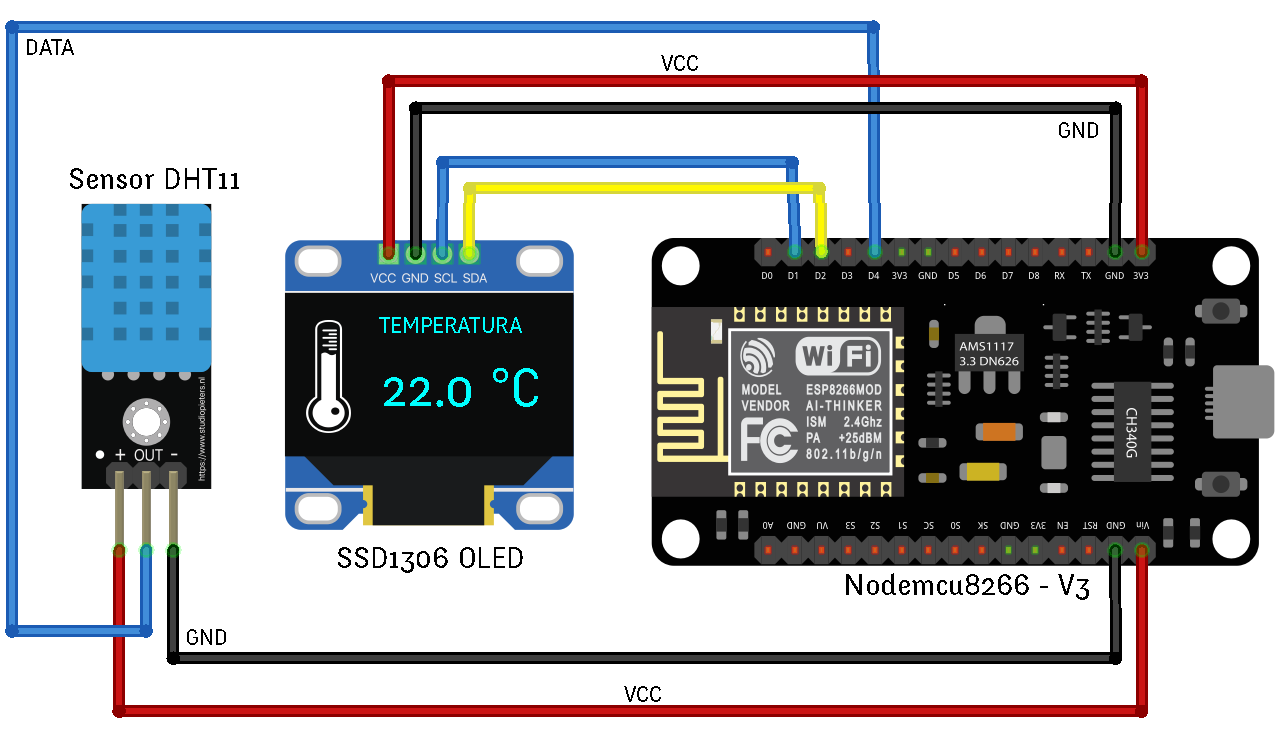
\includegraphics[width=0.85\textwidth]{./Figures/ci-temp.png}
\caption{Esquemático electrónico del módulo de temperatura. }
\label{fig:citemp}
\end{figure}

El proceso de integración total lo podemos ver en las fotografías que se visualizan en la figura \ref{fig:entemp}.

\begin{figure}[htpb]
\centering 
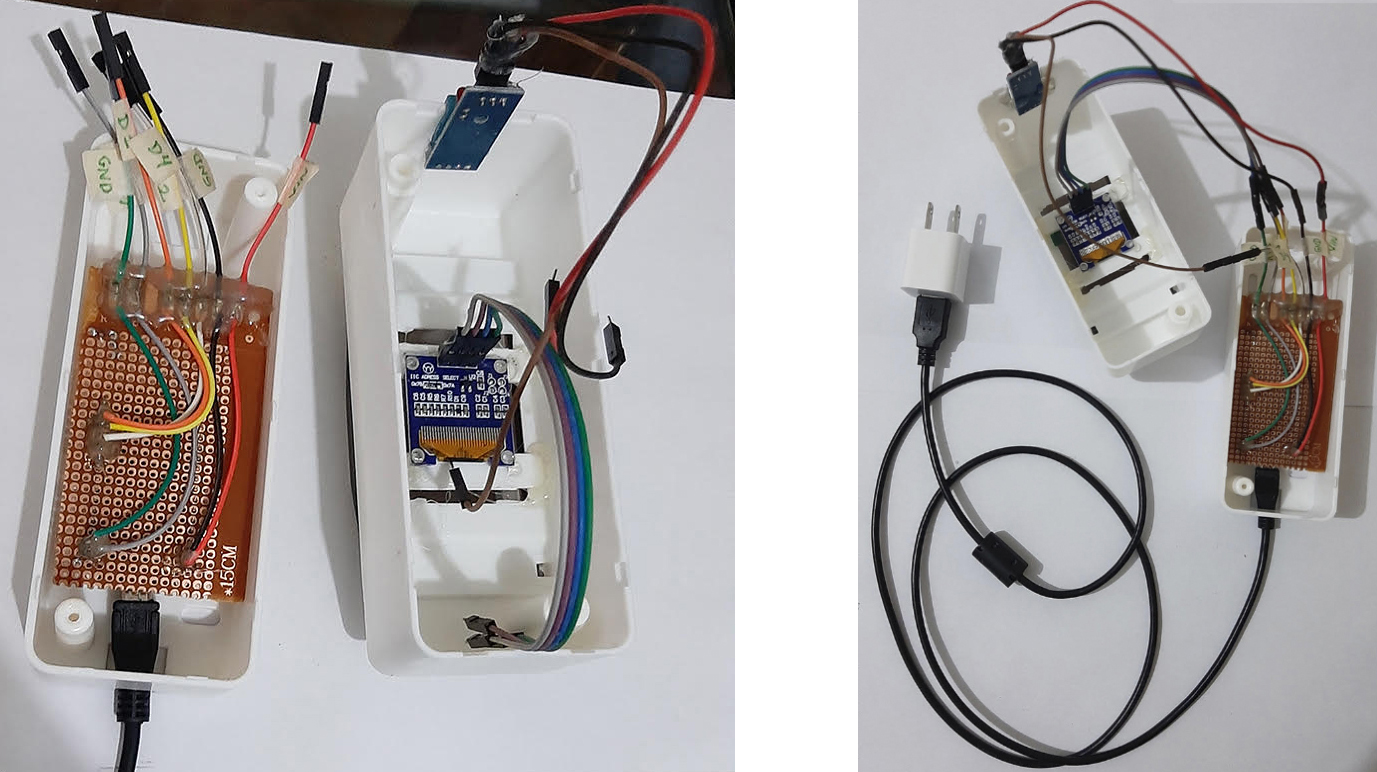
\includegraphics[width=0.95\textwidth]{./Figures/temperatura.jpg}
\caption{Ensamblado del módulo de temperatura. }
\label{fig:entemp}
\end{figure}

\section{Módulo actuador}

Este módulo permite activar o desactivar el paso de la corriente eléctrica dentro de un tomacorriente. La acción de cambio de estados (activado o desactivado) se realiza desde un switch en la interfaz de la aplicación web de monitoreo y control.

Para la construcción del módulo se utilizó una caja (\emph{case}) de tomacorriente  resistente a impactos, de gran durabilidad, autoextinguible e ideal para conductos de cables \citep{WEBSITE:18}. Para fijar el tomacorriente se usó una placa modular de soporte. En la figura \ref{fig:caseactuador} se ilustran los componentes mencionados.

Para la activación del relé de 5 V mediante una salida de la placa NodeMCU8266 fue necesario usar un convertidor de tensión DC-DC Step-Up 2 A MT3608, porque las salidas de la placa NodeMCU8266 son de 3.3 V y la activación del relé requiere 5 V para funcionar. El DC-DC Step-Up tiene como función entregar una tensión de salida constante superior a la tensión de entrada, soporta como tensión de entrada entre 2 V a 24 V y tensión de salida entre 2 V a 28 V. La tensión de salida se puede regular mediante un potenciómetro multivuelta \citep{WEBSITE:19}. La figura \ref{fig:esquemaactuador} ilustra el relé de 30 A y el convertidor de tensión utilizado para la solución a este problema.

\begin{figure}[htpb]
\centering 
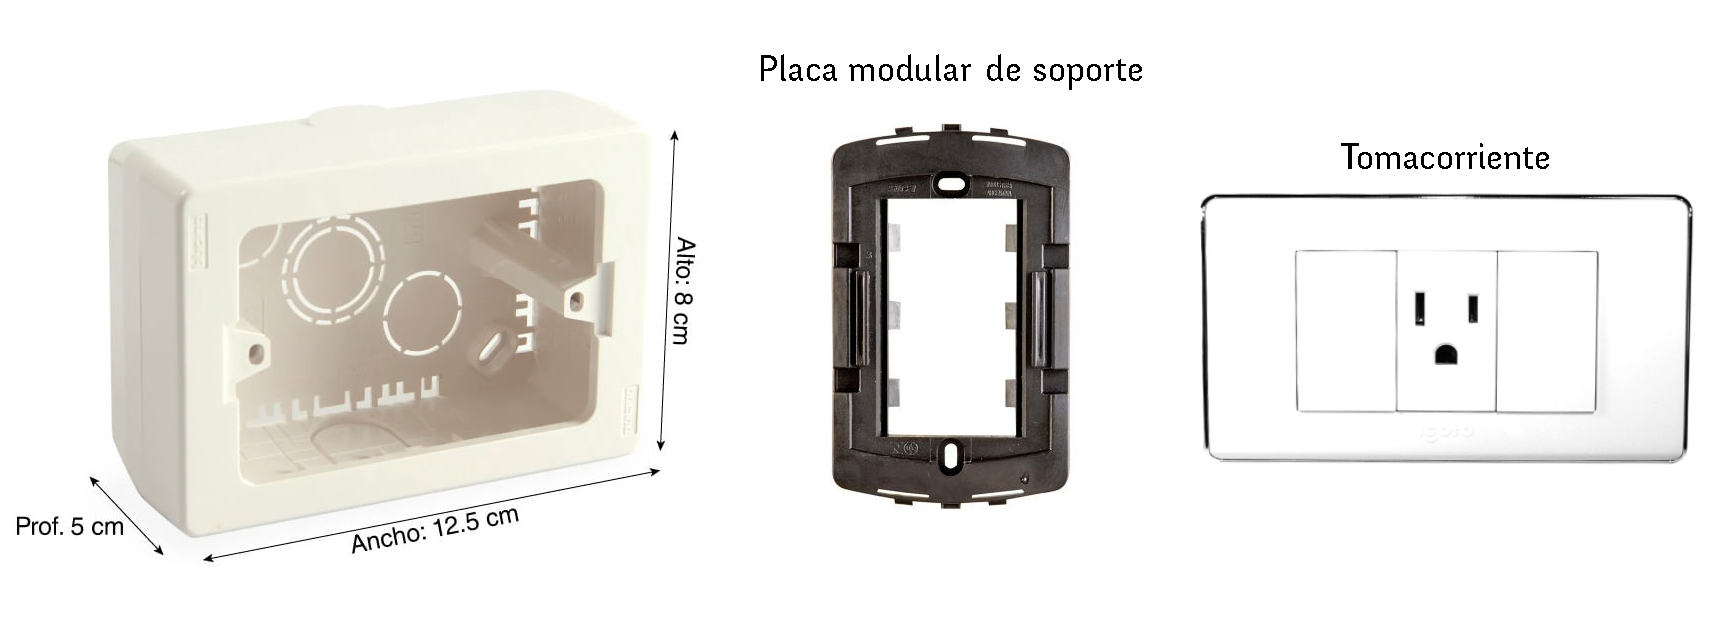
\includegraphics[width=1.0\textwidth]{./Figures/actuador.jpg}
\caption{Case del módulo actuador.}
\label{fig:caseactuador}
\end{figure}


\begin{figure}[htpb]
\centering 
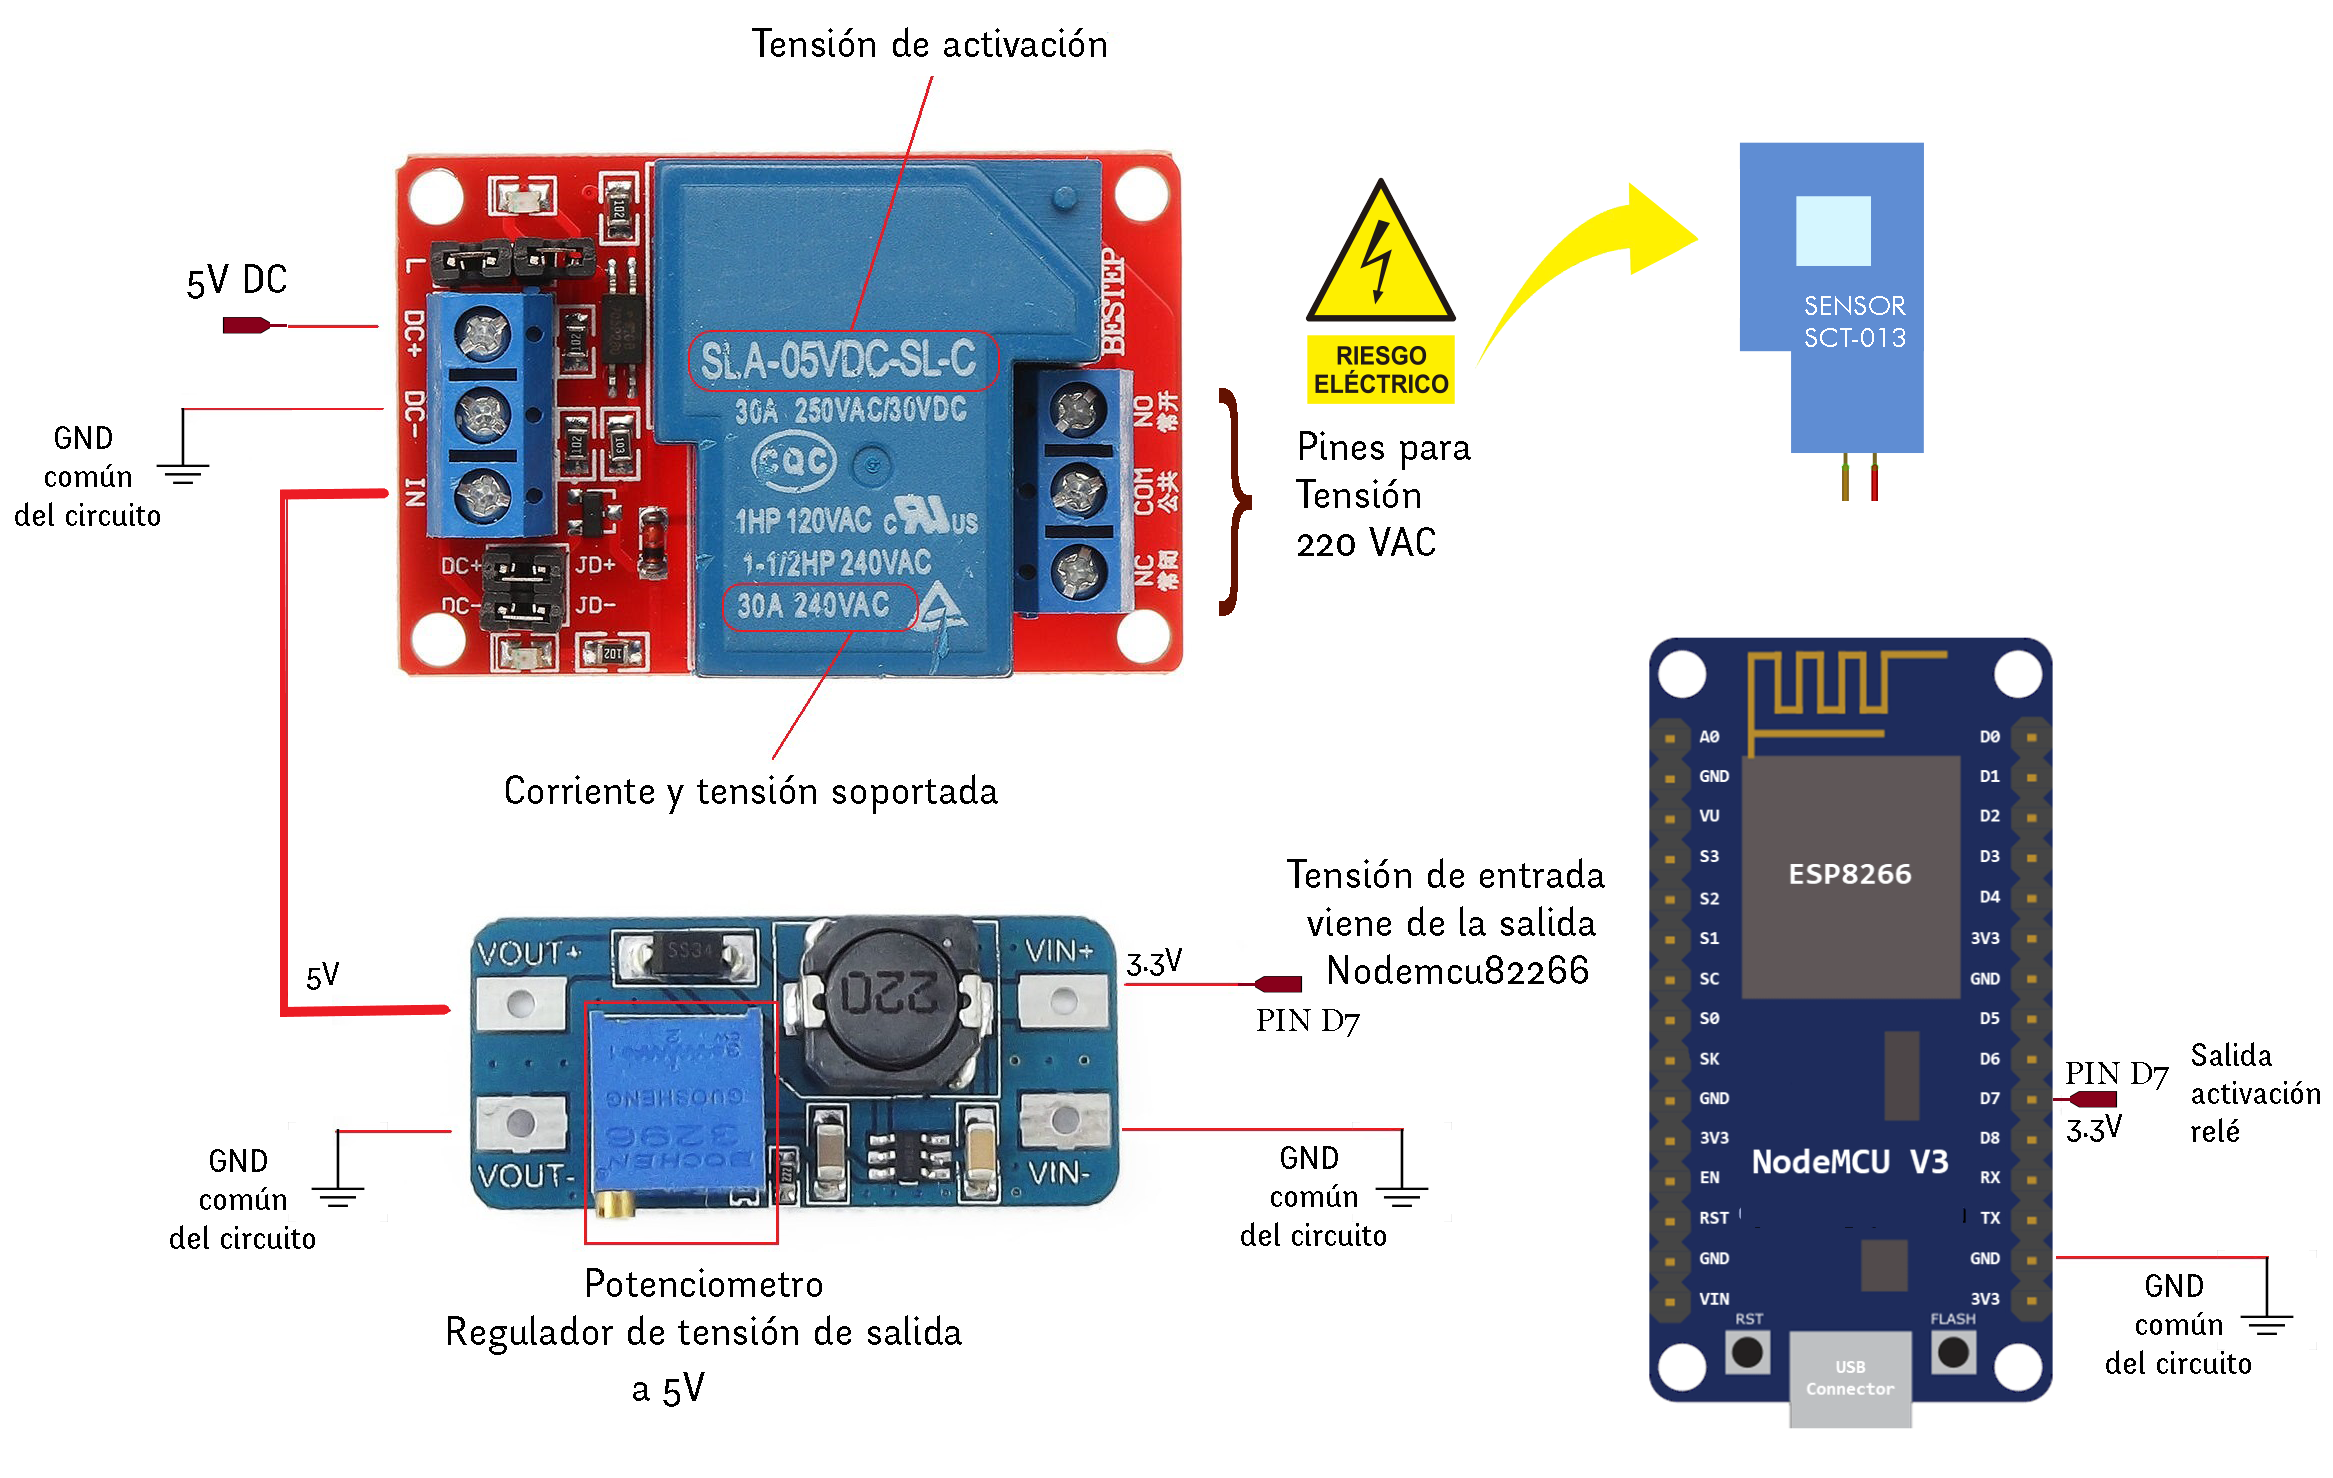
\includegraphics[width=1.0\textwidth]{./Figures/esquemaactuador.png}
\caption{Uso del Step-Up DC-DC para activación del relé. }
\label{fig:esquemaactuador}
\end{figure}

%\vspace{1cm}
%\vspace{1cm}

\section{Módulo de consumo eléctrico}

Este módulo es el responsable de medir el consumo de energía eléctrica dentro de un hogar, oficina o edificio. La integración de los componentes representó un gran reto dentro del proceso de construcción y desarrollo por ser un módulo que permite comunicación bidireccional con el servidor local y a su vez tener sincronización con todos los clientes conectados al sistema.

\vspace{2cm}

\keyword{Cálculo de consumo de energía eléctrica}

La energía eléctrica que consume un artefacto eléctrico, se determina multiplicando la potencia de dicho artefacto por la cantidad de horas que está encendido \citep{BOOK:3}. Por ejemplo ver la ecuación \ref{eq:consumoform}.

\begin{equation}
	\label{eq:consumoform}
	EC = \left( P \cdot T \right)
\end{equation}

\vspace{0.1cm}
Siendo las variables y unidades:
\begin{itemize}
\item EC: energía consumida (kWh)
\item T: tiempo que esta encendido (h)
\item P: potencia eléctrica del artefacto (kW)
\end{itemize}

\vspace{0.1cm}
\keyword{Cálculo de la potencia eléctrica}

El cálculo de la potencia eléctrica se obtiene multiplicando la carga eléctrica, también conocida como tensión eléctrica, que pasa en un instante de tiempo a través de una diferencia de potencia, denominada intensidad. El resultado, cuya unidad es el vatio (en inglés, watt) su símbolo es la W, se obtiene al multiplicar la tensión por la intensidad. La tensión se pone en Voltios (V) y la intensidad en Amperios (A). La fórmula de la potencia eléctrica se ilustra en la ecuación \ref{eq:potenciaform} \citep{WEBSITE:20}.

\begin{equation}
	\label{eq:potenciaform}
	P = \left( V \cdot I \right)
\end{equation}

\vspace{0.2cm}
Siendo las variables y unidades:
\begin{itemize}
\item V: tension eléctrica (V)
\item I: intensidad eléctrica (A)
\item P: potencia eléctrica del artefacto (W)
\end{itemize}


Como se observa en la ecuación \ref{eq:potenciaform}, para poder medir el consumo eléctrico se necesita medir la tensión (V) y la intensidad (A), para lo que se utilizaron los sensores SCT-013-030 y  AC - ZMPT101B, respectivamente.

Los aspectos más importantes para el diseño, desarrollo y construcción del módulo de consumo eléctrico se describen  a continuación, así como el proceso que se usó para almacenar y calcular los consumos eléctricos.


\begin{enumerate}
\item \keyword{Componentes para la construcción del módulo}

Los elementos necesarios son:
\begin{itemize}
\item Gabinete de protección
\item Sensor de tensión eléctrica AC - ZMPT101B
\item Sensor de corriente eléctrica SCT-013-030
\item Convertidor ADC ADS1115
\item Cable de calibre 14
\item Fusible de 30 A
\item Pantalla gráfica LCD
\item Fuente embebida con entrada 220 V y salida de 5 V
\item Leds ultra brillantes:
\end{itemize}

\item \keyword{Aplicación del sensor SCT-013-030}

Para este trabajo se utilizó el sensor de salida por tensión, el SCT-013-030 para corrientes máximas de 30 A (30 A /1 V) y salida en tensión de 1 V.A. Es importante disponer un rango amplio de medición, pero hay que tener en cuenta que un modelo de mayor intensidad se traducirá en una menor precisión. Una intensidad de 30 A a 230 V corresponde con una carga de 6.900 W, potencia suficiente para la mayoría de usuarios domésticos. En la figura \ref{fig:consumo1} se ilustra el esquema lógico a usar y la pinza del sensor.
\vspace{1.0cm}
\begin{figure}[htpb]
\centering 
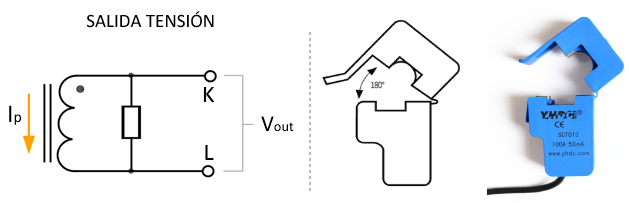
\includegraphics[width=0.9\textwidth]{./Figures/consumo1.png}
\caption{Circuito y pinza del sensor de corriente. }
\label{fig:consumo1}
\end{figure}

El proceso de ensamblado se ilustra en las fotografías de la figura \ref{fig:armadoactuador}.

\begin{figure}[htpb]
\centering 
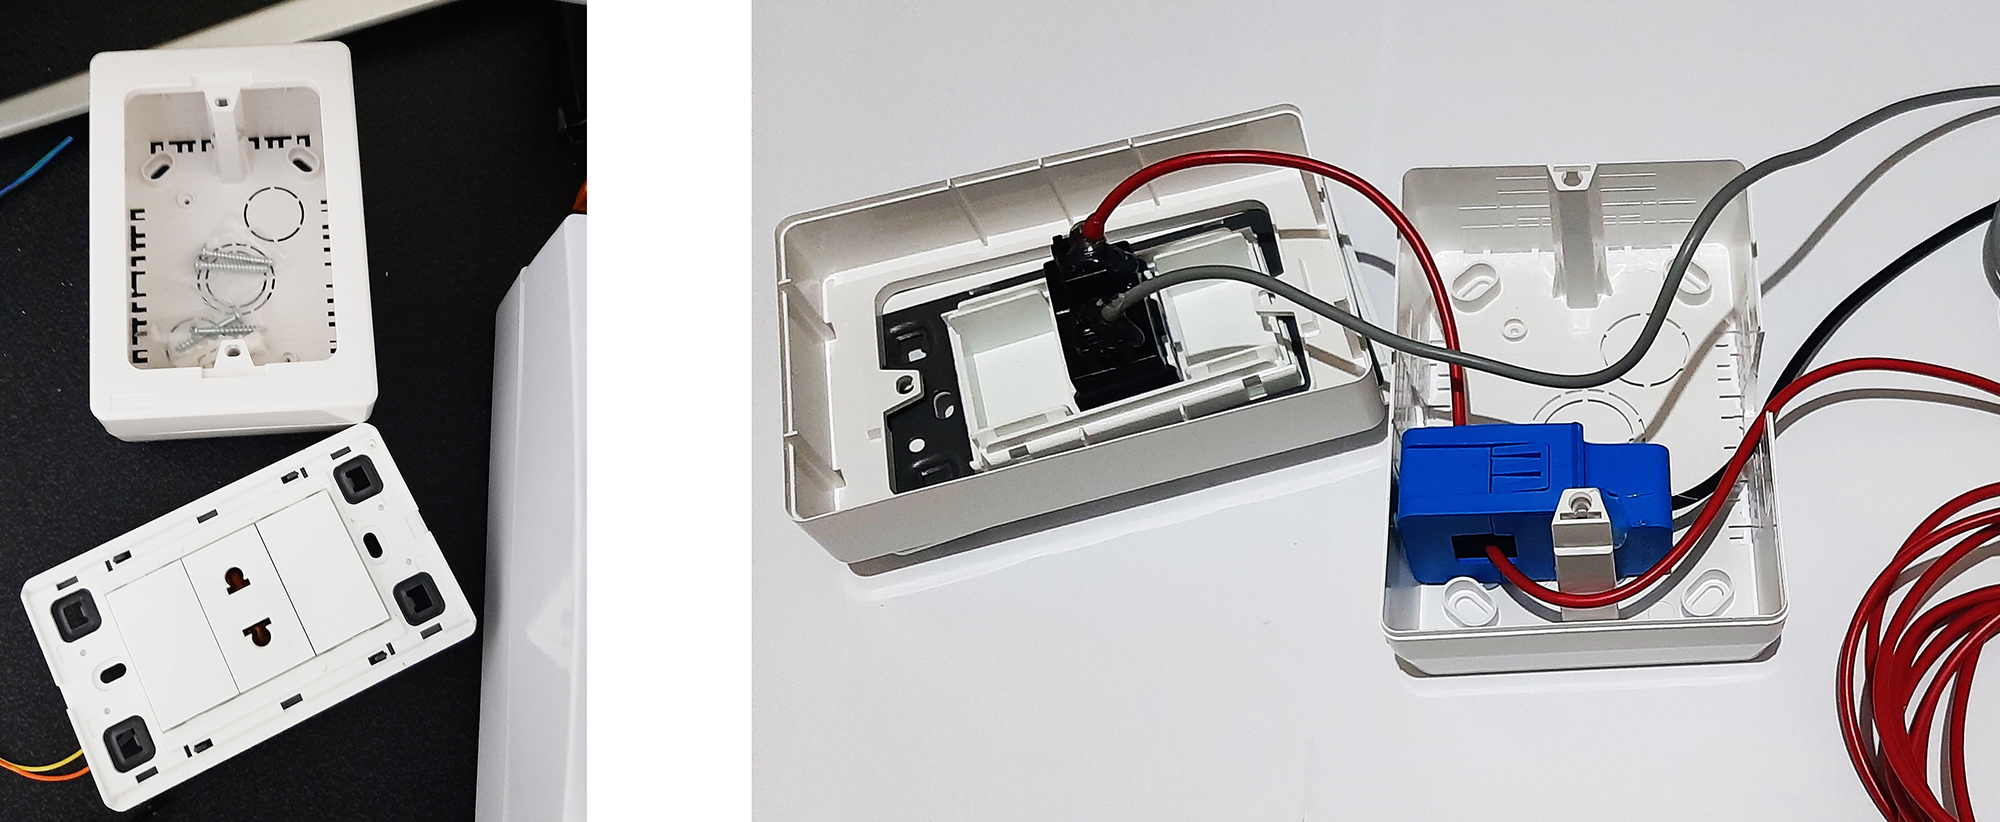
\includegraphics[width=0.85\textwidth]{./Figures/armadoactuador.jpg}
\caption{Ensamblado del módulo actuador. }
\label{fig:armadoactuador}
\end{figure}


\item \keyword{Medición del consumo eléctrico}

Para determinar la potencia eléctrica consumida, el sistema recolecta mediciones del sensor de consumo y realiza la operación matemática de la formula \ref{eq:potenciaform}. Los resultados los almacena de forma periódica (aproximadamente cada 2 segundos) en la base de datos local y remota. Los datos son agrupados según la hora de lectura junto a su respectiva fecha. La tabla \ref{tab:tablaconsumos} muestra la lógica de registros.




\begin{table}[h]
	\centering
	\caption[Registros de consumos]{Registros de consumos}
	\begin{tabular}{l c c }     
		\toprule
		\textbf{Potencia electrodoméstico} & \textbf{Respaldo} &\textbf{Fecha} \\
		\midrule
		Potencia media del ventilador (Pmv) & 10:00 am & 01/02/2022\\		
		Potencia media del ventilador (Pmv) & 11:00 am &01/02/2022 \\
		Potencia media del ventilador (Pmv) & 2:00 pm & 01/02/2022\\		
		Potencia media del ventilador (Pmv) & 3:00 pm & 01/02/2022\\		
		
		\bottomrule
		\hline
	\end{tabular}
	\label{tab:tablaconsumos}
\end{table}

Cada agrupación tiene un aproximado de 1800 registros temporales registrados en una determinada hora. Si se considera como ejemplo los datos de la tabla \ref{tab:tablaconsumos}, el consumo del ventilador en el día 01/02/2022 se calcula usando la formula \ref{eq:consumoform}, dando como resultado la ecuación \ref{eq:potenciaformejemplo2}.

\begin{equation}
	\label{eq:potenciaformejemplo2}
	EC =  \left( P \cdot T \right) = \left(Pmv \cdot 4 \right)
\end{equation}

Los valores del consumo total serán usados para generar la facturación mensual por consumo eléctrico. La figura \ref{fig:modconsumo} muestra la construcción del módulo de consumo.

\begin{figure}[htpb]
\centering 
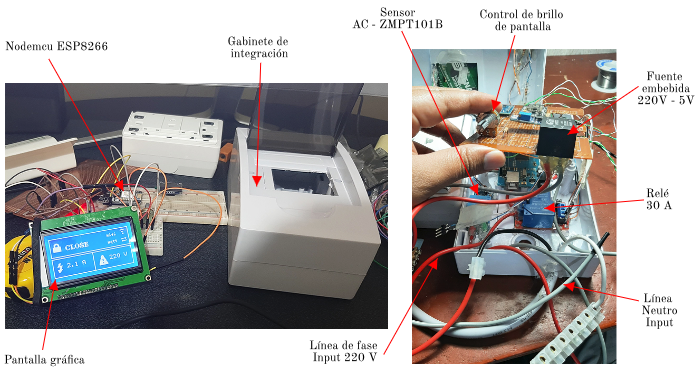
\includegraphics[width=1.0\textwidth]{./Figures/moduloconsumo.png}
\caption{Construcción del módulo de consumo.}
\label{fig:modconsumo}
\end{figure}


\end{enumerate}
\section{Módulo réplica}
Este módulo contiene una copia del software de monitoreo y control pero con la diferencia que se ejecuta en la nube usando los servicios de un servidor y un broker remoto.

%\vspace{1.0cm}



%%%%%%%%%%%%%%%%%%%%%%%%%%%%%%%%%%%%%%%%%%%%%%%%%%%%%%%%%%%%%%%%%%%%%%%%%%%%%
%\begin{landscape} % esto es para rotar la pagina e imagen
%\begin{figure}[htpb]
%\centering 
%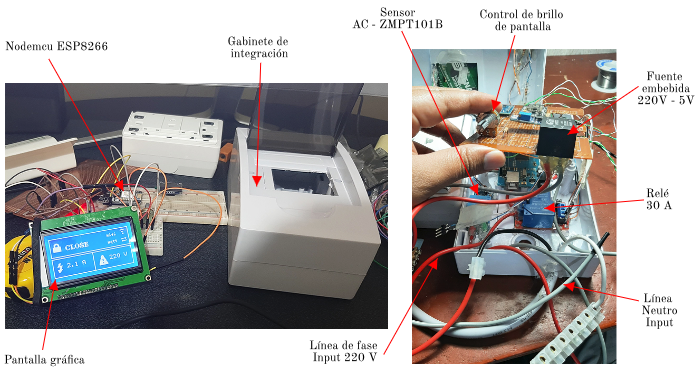
\includegraphics[width=1.5\textwidth]{./Figures/moduloconsumo.png}
%\caption{Construcción del módulo de consumo.}
%\label{fig:modconsumo}
%\end{figure}
%\end{landscape} % 
%%%%%%%%%%%%%%%%%%%%%%%%%%%%%%%%%%%%%%%%%%%%%%%%%%%%%%%%%%%%%%%%%%%%%%%%%%%%%%
\section{Diseño de la red física local}

Para esta tarea se agregó un router inalámbrico como punto de acceso adicional a la red local, sirviendo como medio de comunicación exclusivo de los sensores y actuadores del sistema dentro de la red interna del hogar o edificio. La figura \ref{fig:diagramared} ilustra el diseño físico de la red utilizada.



\section{Configuración de la red WLAN}

El diseño y la configuración de la red WLAN tiene un rol fundamental dentro del desempeño del sistema porque permite garantizar un canal de comunicación seguro, sin interferir la red doméstica.

%Las consideraciones de seguridad para una configuración Wi-Fi segura fueron:

%\begin{itemize}
%\item Uso de un AP (\emph{Access Point}) como elemento central para el servicio Wi-Fi independiente (dedicado solo para el sistema IoT) para garantizar una subred paralela al usado para la red doméstica.
%\item Configuración ideal del canal de comunicación inalámbrica, para evitar el uso de un canal con alto grado de solapamiento.
%\item Uso de dispositivos AP con la función de seguridad de clave WPA2-PSK (AES).
%\item Configurar el nombre de la señal por defecto, la clave de acceso al AP y a la señal Wi-Fi, considerando letras minúsculas, mayúsculas, números y símbolos especiales.
%\item Monitoreo continuo de la red Wi-Fi del AP, para supervisar la presencia únicamente de solo dispositivos válidos en la red dedicada.
%\end{itemize}

\subsection{Configuración del Router inalámbrico}
Los principales criterios de configuración del router inalámbrico a considerar son la seguridad de la señal y la elección del canal para la comunicación Wi-Fi. Para el presente trabajo se usó un \emph{Router/Access Point} (AP) de alta ganancia 300 Mbps SATRA, porque ofrece tasas de transferencia de datos de 300 Mbps y garantiza una cobertura inalámbrica sin cortes tanto en la red del hogar como de la oficina y es compatible con el estándar de encriptación WPA2 (\emph{Wi-Fi Protected Access 2}), diseñado para proteger a la red de ataques externos en un nivel más alto \citep{WEBSITE:25}. La figura \ref{fig:router} muestra el modelo del router SATRA.

\begin{figure}[htpb]
\centering 
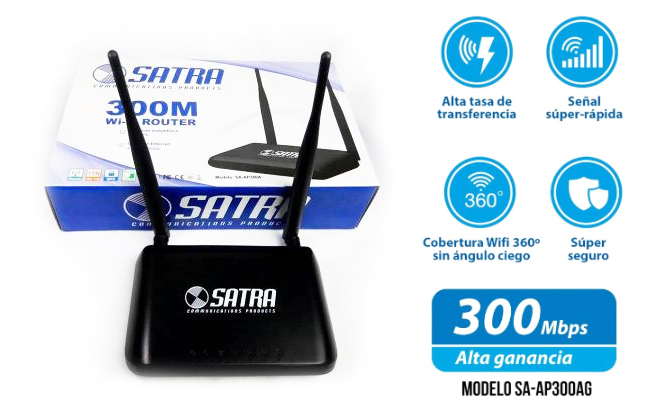
\includegraphics[width=0.7\textwidth]{./Figures/router.jpg}
\caption{Modelo del router utilizado para el diseño de red.}
\label{fig:router}
\end{figure}

Este router tiene tres formas de funcionamiento: AP, router y repetidor. Para nuestro trabajo se seleccionó la configuración AP o punto de acceso. La figura \ref{fig:funcionamientorouter} muestra la configuración del modo de funcionamiento.

Al crear y configurar una red inalámbrica WLAN, es común encontrarse con uno de los problemas más habituales en las redes Wi-Fi, el solapamiento de canales, debido a la gran cantidad de equipos que funcionan en la banda de frecuencia de 2,4 GHz. La mala configuración de red puede ser un motivo para problemas de comunicación Wi-Fi. La conexión a Internet lenta y las desconexiones pueden ocurrir si la red inalámbrica no está configurada correctamente o si hay demasiados dispositivos que están compitiendo por el espacio aéreo inalámbrico de la red. Cada equipo Wi-Fi que cumple con el estándar 802.11 b/g utiliza uno de los 13 canales establecidos de 14 en total y si 2 o más equipos cercanos utilizan el mismo canal, se produce el solapamiento. 
%%%% hasta aqui se revisoooooooooooo 26/04/2022
%%%%%%%%%%%%%%%%%%%%%%%%%%%%%%%%%%%%%%%%%%%%%%%%%%%%%%%%%%%%%%%%%%%%%%%%%%%%%
\begin{landscape} % esto es para rotar la pagina e imagen
\begin{figure}[htpb]
\centering 
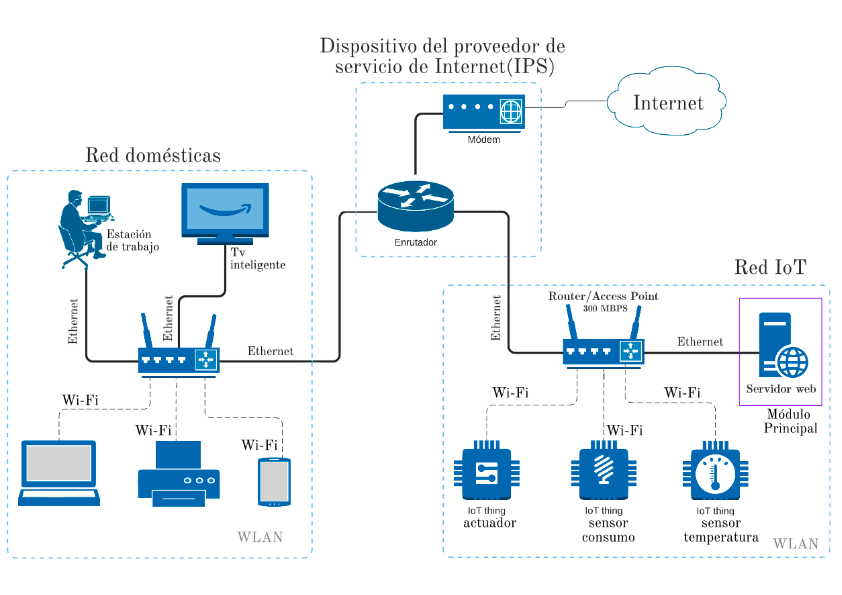
\includegraphics[width=1.3\textwidth]{./Figures/rediot.png}
\caption{Diseño físico de la red WLAN para el sistema IoT.}
\label{fig:diagramared}
\end{figure}
\end{landscape} % 
%%%%%%%%%%%%%%%%%%%%%%%%%%%%%%%%%%%%%%%%%%%%%%%%%%%%%%%%%%%%%%%%%%%%%%%%%%%%%%

Cada canal ocupa un ancho de banda de 22 MHz. El efecto del solapamiento es la bajada en el rendimiento (velocidad) de las redes afectadas \citep{WEBSITE:26}.

\begin{figure}[htpb]
\centering 
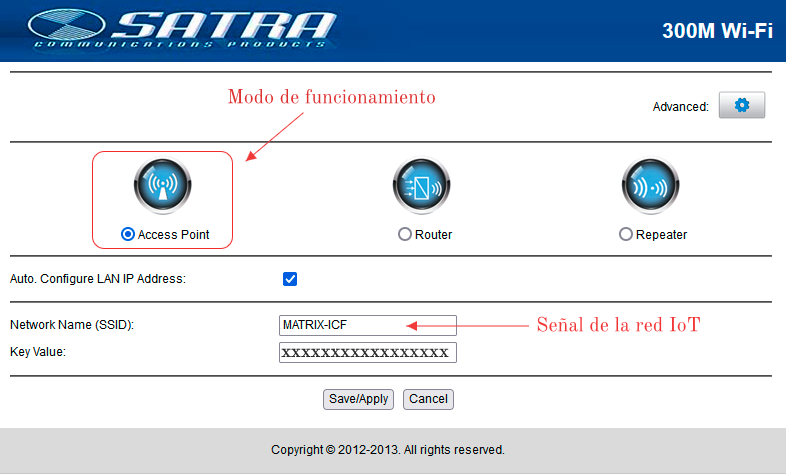
\includegraphics[width=0.7\textwidth]{./Figures/funcionamientorouter.png}
\caption{Elección del modo de funcionamiento del router.}
\label{fig:funcionamientorouter}
\end{figure}

La figura \ref{fig:canales} muestra el ancho de banda utilizado por cada canal y el solapamiento que se produce entre ellos \citep{WEBSITE:27}.

\begin{figure}[htpb]
\centering 
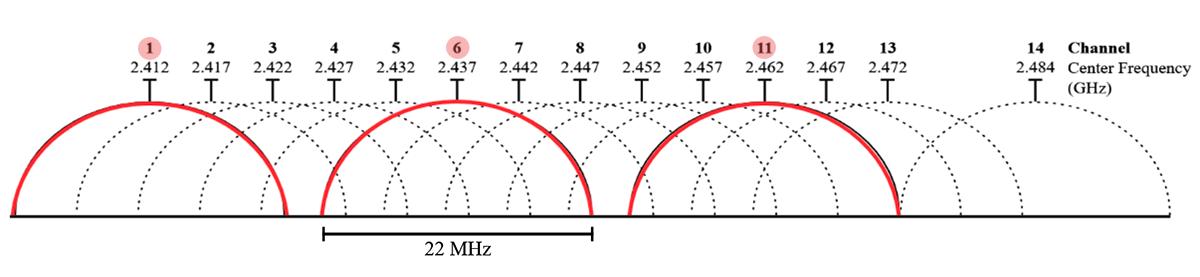
\includegraphics[width=1.0\textwidth]{./Figures/canales.png}
\caption{Diagrama de los canales de 2.4 GHz.}
\label{fig:canales}
\end{figure}

\subsubsection{Elección del canal de comunicación}
En la banda de 2,4 GHz, que por lo general es \emph{Wireless-N}, siempre se elije el canal 1, 11 o 6. Los canales distintos de 1, 11 o 6 recibirán más interferencias. 

Para la elección del canal se tomó en cuenta la figura  \ref{fig:canales} y las siguientes consideraciones \citep{WEBSITE:28}:

\begin{itemize}
\item El canal 1 interferirá y recibirá interferencias de los canales 1-5 de  2,4 GHz.
\item El canal 6 interferirá y recibirá interferencias de los canales 2-10 de  2,4 GHz.
\item El canal 11 interferirá y recibirá interferencias de los canales 7-13 de 2,4 GHz.
\end{itemize}

Utilizando la información anterior, se puede observar que siempre se deben elegir los canales 1, 11 o 6. Si se hace lo contrario, se tendrá la interferencia de más de un canal inalámbrico principal de 2,4 GHz \citep{WEBSITE:28}, ocasionando solapamiento o interferencia en el canal de comunicación de la red IoT a utilizar. Sin embargo, es posible que no se pueda acceder a un canal no interferible, porque pueden existir redes Wi-Fi que estén ocupando los canales 1, 6 y 11. Incluso, pueden existir otras redes vecinas que utilicen canales que se solapen parcialmente y, para estos casos, se debe buscar un canal donde el impacto de ese solapamiento sea mínimo \citep{WEBSITE:27}.

Pare este trabajo la elección del número de canal se fundamentó en la investigación antes mencionada y en la exploración de las redes Wi-Fi vecinas existentes en el entorno donde se implantó el sistema IoT.

\subsubsection{Elección del ancho de banda del canal}

Para la elección de la anchura del canal se establece en 20 MHz para la banda de 2,4 GHz y en automático o en todos los anchos (20 MHz, 40 MHz y 80 MHz) para la banda de 5 GHz \citep{WEBSITE:29}. La anchura del canal especifica el tamaño del ``cauce'' disponible para transferir datos. Los canales más anchos son más rápidos, pero más propensos a sufrir interferencias y a interferir con otros dispositivos. Los 20 MHz para la banda de 2,4 GHz ayudan a evitar problemas de rendimiento y fiabilidad, especialmente cerca de otras redes Wi-Fi y dispositivos de 2,4 GHz, incluidos los dispositivos Bluetooth \citep{WEBSITE:29}. La figura \ref{fig:configuracioncanal} muestra los valores por defecto que tiene el router utilizado y la figura \ref{fig:solapamiento} muestra el solapamiento de las redes inalámbricas locales y vecinas donde se probó el sistema IoT.

\begin{figure}[htpb]
\centering 
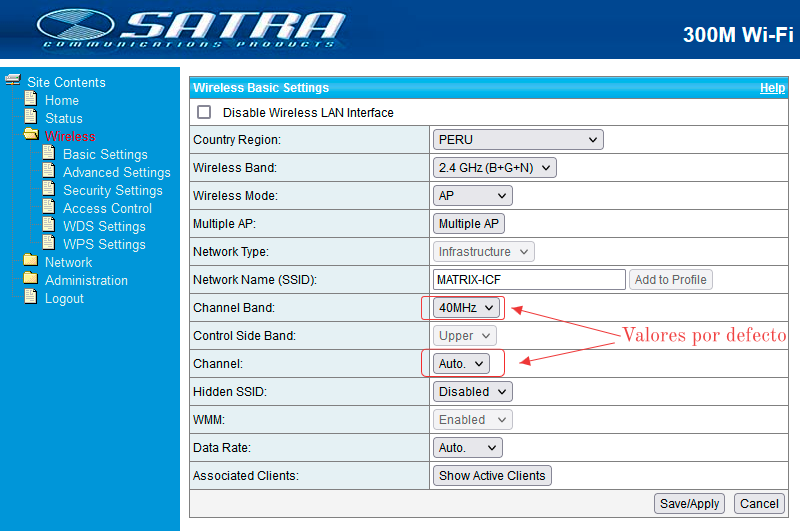
\includegraphics[width=0.9\textwidth]{./Figures/configuracioncanal.png}
\caption{Configuración por defecto del router SATRA.}
\label{fig:configuracioncanal}
\end{figure}

Para los casos donde se amplía el canal (40 MHz), eso significa duplicar las interferencias con las redes vecinas. Para remediarlo, la IEEE introdujo un mecanismo de coexistencia en 2,4 GHz para evitar las molestias a las redes vecinas, muchos fabricantes de routers se han adaptado a la norma, por lo que no permiten que los usuarios seleccionen arbitrariamente los 40 MHz, sino que se limitan a un ``auto 20/40''. Por lo tanto, el router solo utilizará la frecuencia de 40 MHz si los canales vecinos están libres, de lo contrario, utilizará la frecuencia de 20 MHz \citep{WEBSITE:30}.

La figura \ref{fig:configuracionancho} muestra la configuración final elegida para este trabajo. Las pruebas y análisis de canales así como la justificación para su elección se describen en el capítulo 4 de este documento.

%%%%%%%%%%%%%%%%%%%%%%%%%%%%%%%%%%%%%%%%%%%%%%%%%%%%%%%%%%%%%%%%%%%%%%%%%
\begin{landscape} % esto es para rotar la pagina e imagen
\begin{figure}[htpb]
\centering 
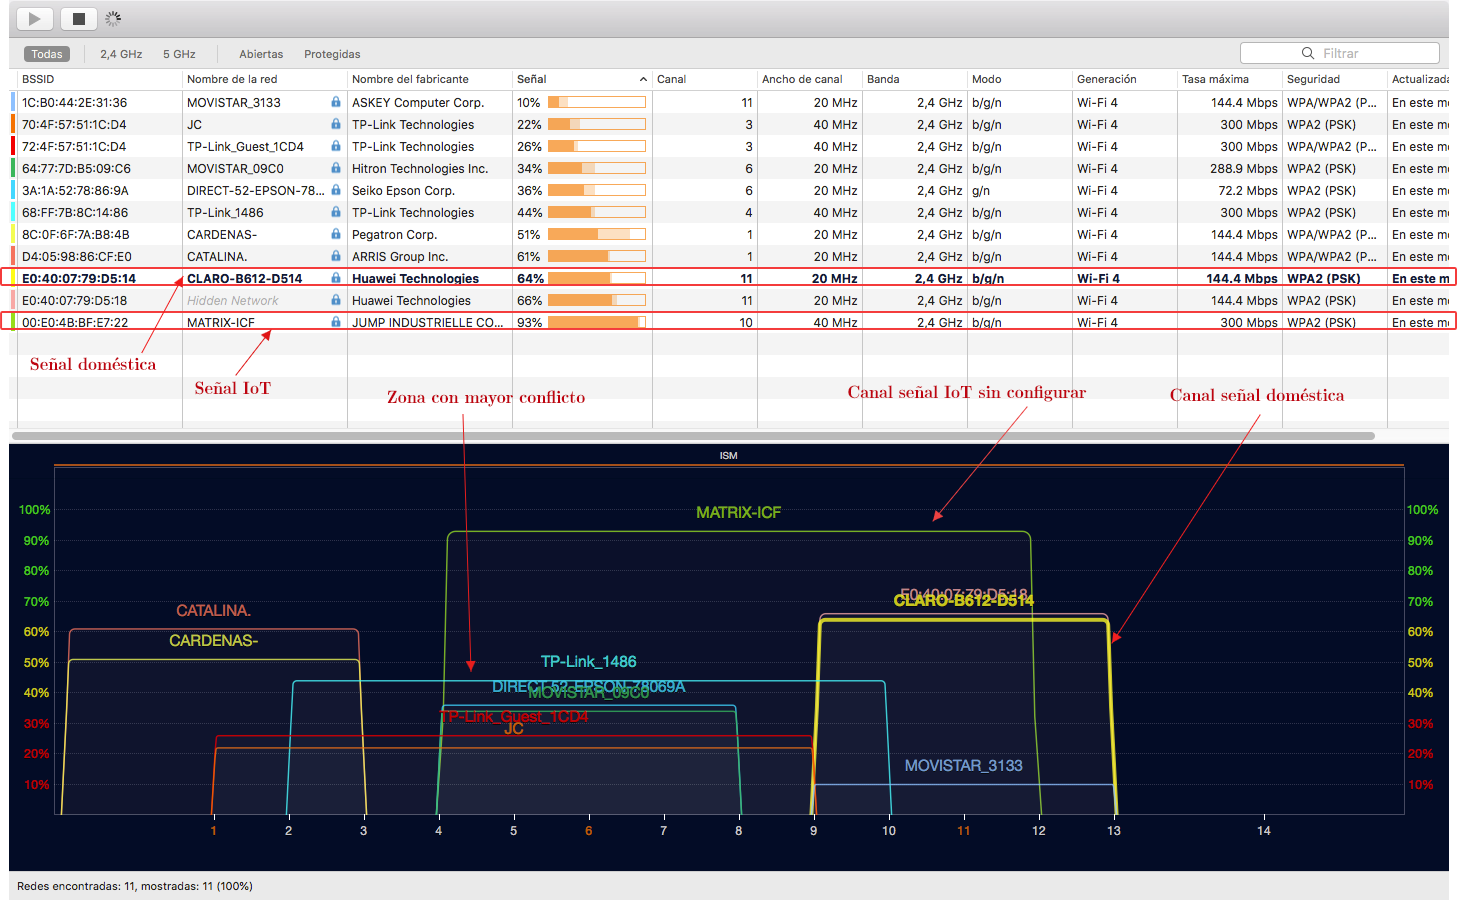
\includegraphics[width=1.5\textwidth]{./Figures/wifi/01-doc.png}
\caption{Solapamiento de canales de las redes inalámbricas locales y vecinas.}
\label{fig:solapamiento}
\end{figure}
\end{landscape} % 
%%%%%%%%%%%%%%%%%%%%%%%%%%%%%%%%%%%%%%%%%%%%%%%%%%%%%%%%%%%%%%%%%%%%%%%%%%%%
\vspace{0.5cm}
\begin{figure}[htpb]
\centering 
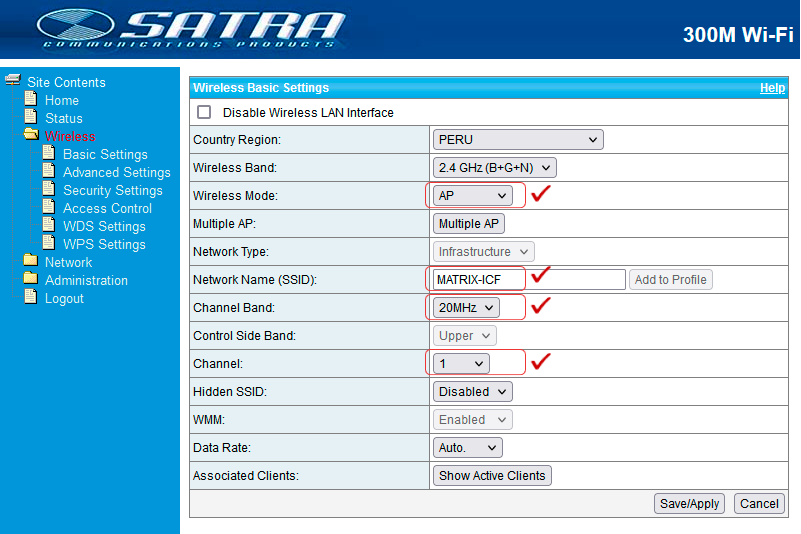
\includegraphics[width=1.0\textwidth]{./Figures/configuracionancho.png}
\caption{Configuración para la red WLAN del sistema IoT.}
\label{fig:configuracionancho}
\end{figure}
%------------------------------------------------

\subsubsection{Configuración de seguridad inalámbrica}
Dentro de los parámetros de seguridad se configuró la opción de autenticación \emph{auth. and encryption}. La figura \ref{fig:encriptacion} ilustra la elección de encriptación y autenticación para el acceso a la señal del AP 
%access point y en la figura \ref{fig:configuracionfinal} Ilustra los resultados finales de la %configuración del access point.

\vspace{0.5cm}
\begin{figure}[htpb]
\centering 
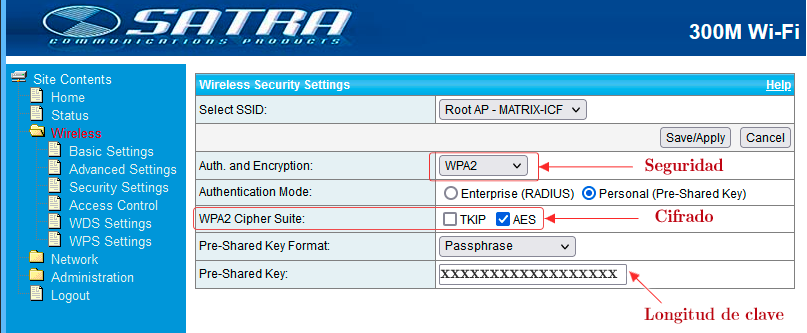
\includegraphics[width=1.0\textwidth]{./Figures/encriptacion.png}
\caption{Configuración de autenticación para la señal Wi-Fi.}
\label{fig:encriptacion}
\end{figure}
%------------------------------------------------------
%\vspace{0.1cm}
%\begin{figure}[htpb]
%\centering 
%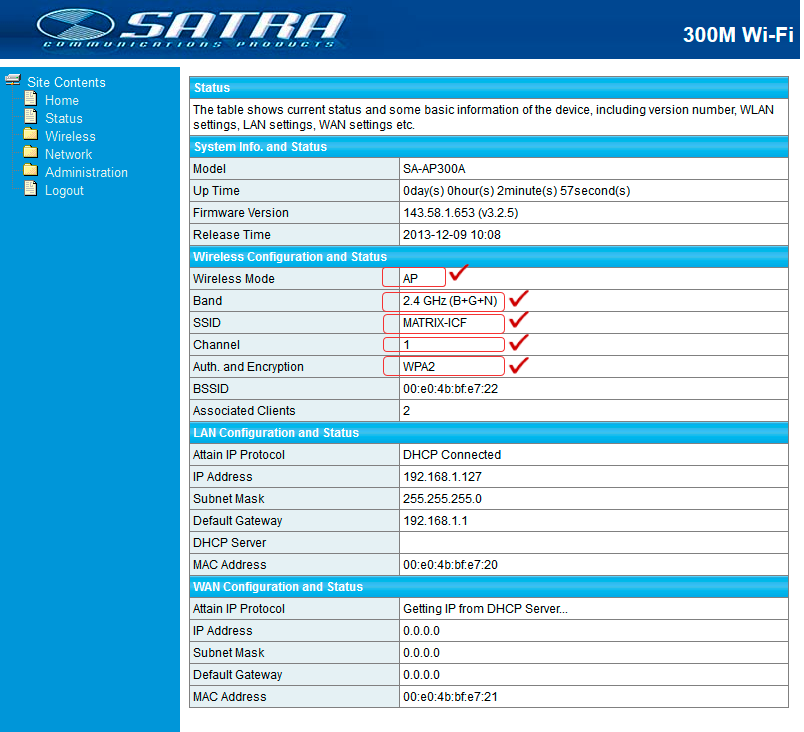
\includegraphics[width=1.0\textwidth]{./Figures/configuracionfinal.png}
%\caption{Resumen de la configuración resultante del router.}
%\label{fig:configuracionfinal}
%\end{figure}

\section{Software para monitoreo y control}

El software desarrollado para este trabajo fue hecho a medida por ser parte fundamental dentro de los objetivos planteados al inicio, como emprendimiento personal. El software es de tipo web y cumple con la característica de ser responsivo para garantizar la adaptación visual a distintos dispositivos del mercado actual. 

%Las consideraciones de seguridad para el \emph{software} de monitoreo fueron:

%\begin{itemize}
%\item Encriptación de claves de acceso, la longitud de cadena de las claves  deben ser mayor a 8 dígitos, considerando números, letras mayúsculas, letras minúsculas, números y símbolos especiales.
%\item Medidas de protección contra \emph{Injeccion SQL} y usar sentencias preparadas u objetos PDO (\emph{PHP Data Objects}) para las conexiones hacia la base de datos.
%\item Control de acceso por CORS (\emph{Cross Origin Resource Sharing}) para recursos de la API REST.
%\item Configuración del archivo .htaccess para evitar listado de directorios o accesos no permitidos.
%\item Minificar los archivos CSS (\emph{Cascading Style Sheets}) y JS (\emph{JavaScript}) de la aplicación web.
%\item Control de acceso al sistema según validación de roles y permisos.
%\item Uso de la programación orientada a objetos.
%\item Uso de peticiones POST como prioridad, si fuera necesario el uso de las peticiones GET, utilizarlas con el paso de parámetros encriptados.
%\end{itemize}



Las figuras \ref{fig:software1} y \ref{fig:software2} muestran los resultados responsivos para cada tipo de dispositivo considerado en el desarrollo.

\begin{figure}[htpb]
\centering 
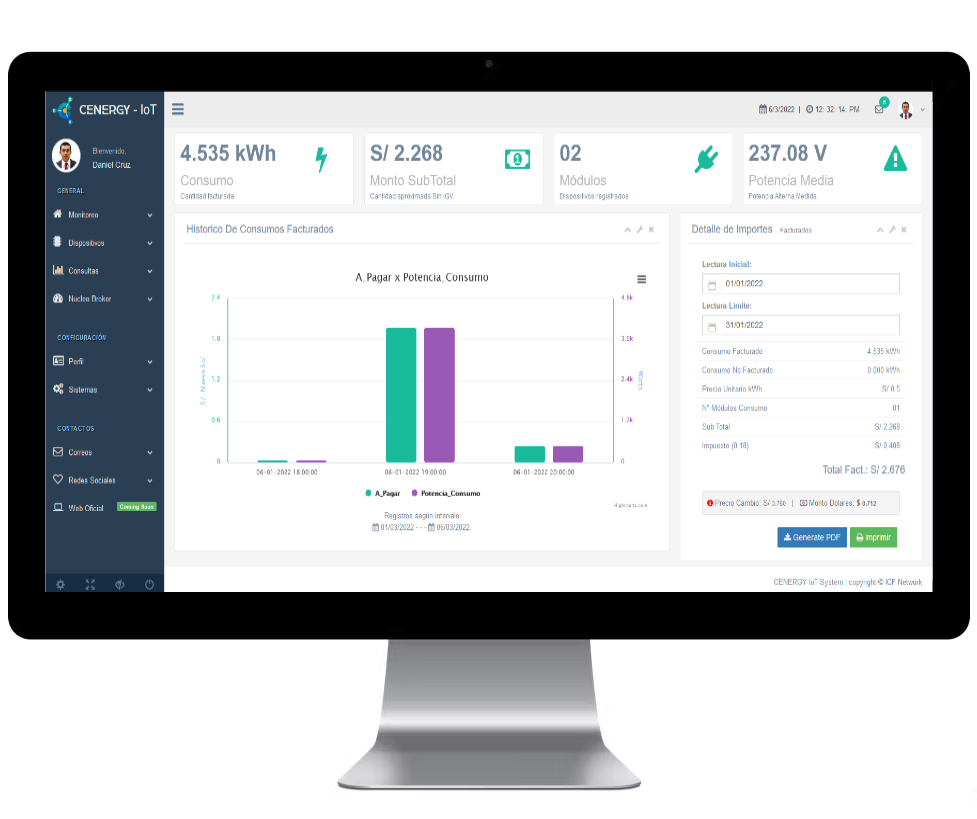
\includegraphics[width=0.62 \textwidth]{./Figures/responsive1.png}
\caption{Vista del software en equipos desktop y laptop.}
\label{fig:software1}
\end{figure}

\vspace{1.0cm}
\begin{figure}[htpb]
\centering 
\includegraphics[width=0.65\textwidth]{./Figures/responsive2.png}
\caption{Vista del software en tableta y celular.}
\label{fig:software2}
\end{figure}

\vspace{1.0cm}
\section{Resultados de los módulos del sistema IoT}
En esta sección se muestran las imágenes reales de los resultados obtenidos de la construcción de cada módulo físico. Estos dispositivos fueron utilizados para las pruebas de validación en un ambiente real IoT. Las figuras \ref{fig:modPrincipal}, \ref{fig:modTemp} y \ref{fig:modConsumo2} muestran los módulos.

 
\begin{figure}[htpb]
\centering 
\includegraphics[width=0.9\textwidth]{./Figures/principal2.png}
\caption{Vista superior y posterior del módulo principal.}
\label{fig:modPrincipal}
\end{figure}



\begin{figure}[htpb]
\centering 
\includegraphics[width=0.85\textwidth]{./Figures/moduloTemp2.png}
\caption{Vista lateral, frente y superior del módulo de temperatura.}
\label{fig:modTemp}
\end{figure}



%%%%%%%%%%%%%%%%%%%%%%%%%%%%%%%%%%%%%%%%%%%%%%%%%%%

\begin{landscape} % esto es para rotar la pagina e imagen
\begin{figure}[htpb]
\centering 
\includegraphics[width=1.8\textwidth]{./Figures/consumo3.png}
\caption{Vista frontal y lateral del módulo actuador y módulo de consumo.}
\label{fig:modConsumo2}
\end{figure}
\end{landscape} %


%%%%%%%%%%%%%%%%%%%%%%%%%%%%%%%%%%%%%%%%%%%%%%%%%%%
\section{Interfaces gráficas del software de monitoreo y control}

El software de monitoreo y control fue diseñado y desarrollado a medida con el objetivo de ser el autor de este trabajo el dueño de los derechos de \emph{Copyright} del mismo, ademas, el \emph{software} por ser de tipo web requiere solo un navegador web y conexión a la red local o a Internet para poder ser utilizado. El software ha sido nombrado como: \emph{Cenergy IoT System} y hace referencia al control de energía eléctrica mediante un sistema IoT. Se espera su evolución y madurez en trabajos futuros. 

%Las principales interfaces gráficas de usuario (GUI) que se muestran a %continuación son el resultado de lo logrado en esta primera versión del %software hasta la fecha de presentación de este trabajo. Las GUIs son:

\begin{itemize}
\item La interfaz de control de acceso al sistema se muestra en la figura \ref{fig:gui0}. Las credenciales utilizadas son el número de su documento nacional de identidad (DNI) y una contraseña de longitud mínima de 8 caracteres.

\item La interfaz de presentación inicial al ingresar al sistema (\emph{dashboard}) se muestra en la figura \ref{fig:gui1}. Esta interfaz muestra el resumen de lo que actualmente está almacenado en la base de datos del sistema. Resalta el consumo facturado y el no facturado a la fecha actual de acceso considerando intervalos de un mes.

\item La interfaz de monitoreo para sensores se muestra en la figura \ref{fig:gui2}. Esta interfaz permite mostrar en tiempo real los sensores que tiene el sistema IoT, así como el estado de los mismos. Si un sensor tiene un estado CONECTADO se podrán observar sus detalles desde la opción ``ver detalles'', pudiendo acceder a una vista gráfica más detallada del mismo, tal como se muestra en la figura \ref{fig:gui2-1}.

\item La interfaz de monitoreo y control para sensores de consumo y sus actuadores se muestran el figura \ref{fig:gui3}. Esta interfaz permite visualizar en tiempo real los módulos registrados y conectados al sistema IoT. Cada módulo en estado CONECTADO muestra el dispositivo que está realizando consumo mediante una señal de onda, junto a su interruptor actuador cuya función es el control del paso o bloqueo de energía eléctrica en el módulo. Si el módulo se encuentra con el estado CONECTADO se podrá observar sus detalles desde la opción ``ver detalles'', pudiendo acceder a una vista gráfica más detallada del mismo, tal como se muestra en la figura \ref{fig:gui3-1}.

\item La interfaz de registro o agregado de módulos al sistema IoT se muestra en la figura \ref{fig:gui4}. Para el registro cada módulo cuenta con un código y número de módelo, para su identificación dentro del sistema.

\item El software actualmente presenta interfaces para cuatro tipos de consultas, que son: lecturas de temperatura, historial de temperatura, consumo sin facturar y consumo facturado. Cada lectura que se registra como consumo en la base de datos se respalda en agrupaciones de intervalos de horas y los registros que aún no completan las horas, podrán ser consultados desde las opciones: lectura de temperatura y consumos sin facturar. Los resultados de las consultas podrán ser exportados en formatos excel o pdf y, si se desea, ser impresos directamente. La figura \ref{fig:gui5} muestra la interfaz de consultas.

\item El software cuenta con una interfaz que muestra un grafo que permite visualizar en tiempo real la comunicación de los módulos así como los mensajes entre canales. El grafo se muestra en la figura \ref{fig:grafo}.


\end{itemize}






%%%%%%%%%%%%%%%%%%%%%%%%%%%%%%%%%%%%%%%%%%%%%%%%%%%
\begin{landscape} % esto es para rotar la pagina e imagen
\begin{figure}[htpb]
\centering 
\includegraphics[width=1.55\textwidth]{./Figures/gui/0.png}
\caption{Interfaz gráfica de usuario de acceso al software de monitoreo y control.}
\label{fig:gui0}
\end{figure}
\end{landscape} %

%%%%%%%%%%%%%%%%%%%%%%%%%%%%%%%%%%%%%%%%%%%%%%%%%%%

%%%%%%%%%%%%%%%%%%%%%%%%%%%%%%%%%%%%%%%%%%%%%%%%%%%
\begin{landscape} % esto es para rotar la pagina e imagen
\begin{figure}[htpb]
\centering 
\includegraphics[width=1.55\textwidth]{./Figures/gui/1.png}
\caption{Dashboard inicial del software de monitoreo y control.}
\label{fig:gui1}
\end{figure}
\end{landscape} %

%%%%%%%%%%%%%%%%%%%%%%%%%%%%%%%%%%%%%%%%%%%%%%%%%%%

%%%%%%%%%%%%%%%%%%%%%%%%%%%%%%%%%%%%%%%%%%%%%%%%%%%
\begin{landscape} % esto es para rotar la pagina e imagen
\begin{figure}[htpb]
\centering 
\includegraphics[width=1.55\textwidth]{./Figures/gui/2.png}
\caption{Interfaz gráfica de usuario donde se listan los sensores del sistema.}
\label{fig:gui2}
\end{figure}
\end{landscape} %

%%%%%%%%%%%%%%%%%%%%%%%%%%%%%%%%%%%%%%%%%%%%%%%%%%%

%%%%%%%%%%%%%%%%%%%%%%%%%%%%%%%%%%%%%%%%%%%%%%%%%%%
\begin{landscape} % esto es para rotar la pagina e imagen
\begin{figure}[htpb]
\centering 
\includegraphics[width=1.5\textwidth]{./Figures/gui/2-1.png}
\caption{Interfaz gráfica de usuario donde se muestran todos los detalles de un sensor.}
\label{fig:gui2-1}
\end{figure}
\end{landscape} %

%%%%%%%%%%%%%%%%%%%%%%%%%%%%%%%%%%%%%%%%%%%%%%%%%%%

%%%%%%%%%%%%%%%%%%%%%%%%%%%%%%%%%%%%%%%%%%%%%%%%%%%
\begin{landscape} % esto es para rotar la pagina e imagen
\begin{figure}[htpb]
\centering 
\includegraphics[width=1.52\textwidth]{./Figures/gui/3.png}
\caption{Interfaz gráfica de usuario donde se listan los sensores de consumo junto a su función de actuador.}
\label{fig:gui3}
\end{figure}
\end{landscape} %

%%%%%%%%%%%%%%%%%%%%%%%%%%%%%%%%%%%%%%%%%%%%%%%%%%%

%%%%%%%%%%%%%%%%%%%%%%%%%%%%%%%%%%%%%%%%%%%%%%%%%%%
\begin{landscape} % esto es para rotar la pagina e imagen
\begin{figure}[htpb]
\centering 
\includegraphics[width=1.52\textwidth]{./Figures/gui/3-1.png}
\caption{Interfaz gráfica de usuario donde se muestran todos los detalles de un sensor de consumo.}
\label{fig:gui3-1}
\end{figure}
\end{landscape} %

%%%%%%%%%%%%%%%%%%%%%%%%%%%%%%%%%%%%%%%%%%%%%%%%%%%

%%%%%%%%%%%%%%%%%%%%%%%%%%%%%%%%%%%%%%%%%%%%%%%%%%%
\begin{landscape} % esto es para rotar la pagina e imagen
\begin{figure}[htpb]
\centering 
\includegraphics[width=1.55\textwidth]{./Figures/gui/4.png}
\caption{Interfaz gráfica de usuario para agregar un nuevo dispositivo al sistema.}
\label{fig:gui4}
\end{figure}
\end{landscape} %

%%%%%%%%%%%%%%%%%%%%%%%%%%%%%%%%%%%%%%%%%%%%%%%%%%%

%%%%%%%%%%%%%%%%%%%%%%%%%%%%%%%%%%%%%%%%%%%%%%%%%%%
\begin{landscape} % esto es para rotar la pagina e imagen
\begin{figure}[htpb]
\centering 
\includegraphics[width=1.5\textwidth]{./Figures/gui/5.png}
\caption{Interfaz gráfica de usuario donde se muestran las consultas y reportes de la base de datos.}
\label{fig:gui5}
\end{figure}
\end{landscape} %

%%%%%%%%%%%%%%%%%%%%%%%%%%%%%%%%%%%%%%%%%%%%%%%%%%%
\begin{landscape} % esto es para rotar la pagina e imagen
\begin{figure}[htpb]
\centering 
\includegraphics[width=1.5\textwidth]{./Figures/gui/nucleo.png}
\caption{Grafo de comunicación y sincronización del núcleo del sistema IoT.}
\label{fig:grafo}
\end{figure}
\end{landscape} %
% Chapter Template

\chapter{Ensayos y resultados} % Main chapter title

\label{Chapter4} % Change X to a consecutive number; for referencing this chapter elsewhere, use \ref{ChapterX}


%----------------------------------------------------------------------------------------
%	SECTION 1
%----------------------------------------------------------------------------------------
En este capítulo se detallan los resultados esperados y obtenidos sobre cada prueba empleada para validar la integración del sistema y poder comprobar que el alcance funciona logrado es acorde a los esperado.
\citep{ARTICLE:1}, \citep{BOOK:1}, \citep{BOOK:2}, \citep{WEBSITE:1}.
\section{Banco de pruebas}

Todos los ensayos que se describen en este capítulo fueron efectuados utilizando el diseño físico de red que se muestra en la fig.....  Los pruebas de funcionalidad remota se realizo usando un dispositivo móvil con acceso a la red celular mediante el uso de paquete de datos de Internet.

\begin{figure}[htbp]
	\centering
	\includegraphics[width=0.91\textwidth]{./Figures/banco2.png}
	\caption{Esquema del banco de pruebas utilizado.}

	\label{fig:banco}
\end{figure}


\section{Resultados de los módulos del sistema IoT}

fotos del modulo principal.

\begin{figure}[htpb]
\centering 
\includegraphics[width=0.95\textwidth]{./Figures/principal2.png}
\caption{Vista superior y posterior del módulo principal.}
\label{fig:modPrincipal}
\end{figure}

foto del modulo de temperatura.

\begin{figure}[htpb]
\centering 
\includegraphics[width=0.9\textwidth]{./Figures/moduloTemp.png}
\caption{Vista lateral, frente y superior del módulo de temperatura.}
\label{fig:modTemp}
\end{figure}

foto del modulo actuador y consumo.

%%%%%%%%%%%%%%%%%%%%%%%%%%%%%%%%%%%%%%%%%%%%%%%%%%%

\begin{landscape} % esto es para rotar la pagina e imagen
\begin{figure}[htpb]
\centering 
\includegraphics[width=1.8\textwidth]{./Figures/consumo2.png}
\caption{Vista frontal y lateral del módulo actuador y módulo de consumo.}
\label{fig:modConsumo2}
\end{figure}
\end{landscape} %


%%%%%%%%%%%%%%%%%%%%%%%%%%%%%%%%%%%%%%%%%%%%%%%%%%%
\section{Interfaces gráficas del sistema de monitoreo}

%%%%%%%%%%%%%%%%%%%%%%%%%%%%%%%%%%%%%%%%%%%%%%%%%%%
\begin{landscape} % esto es para rotar la pagina e imagen
\begin{figure}[htpb]
\centering 
\includegraphics[width=1.55\textwidth]{./Figures/gui/0.png}
\caption{Interfaz gráfica de usuario de acceso al software de monitoreo y control.}
\label{fig:gui0}
\end{figure}
\end{landscape} %

%%%%%%%%%%%%%%%%%%%%%%%%%%%%%%%%%%%%%%%%%%%%%%%%%%%

%%%%%%%%%%%%%%%%%%%%%%%%%%%%%%%%%%%%%%%%%%%%%%%%%%%
\begin{landscape} % esto es para rotar la pagina e imagen
\begin{figure}[htpb]
\centering 
\includegraphics[width=1.55\textwidth]{./Figures/gui/1.png}
\caption{Dashboard inicial del software de monitoreo y control.}
\label{fig:gui1}
\end{figure}
\end{landscape} %

%%%%%%%%%%%%%%%%%%%%%%%%%%%%%%%%%%%%%%%%%%%%%%%%%%%

%%%%%%%%%%%%%%%%%%%%%%%%%%%%%%%%%%%%%%%%%%%%%%%%%%%
\begin{landscape} % esto es para rotar la pagina e imagen
\begin{figure}[htpb]
\centering 
\includegraphics[width=1.55\textwidth]{./Figures/gui/2.png}
\caption{Interfaz gráfica de usuario donde se listan los sensores del sistema.}
\label{fig:gui2}
\end{figure}
\end{landscape} %

%%%%%%%%%%%%%%%%%%%%%%%%%%%%%%%%%%%%%%%%%%%%%%%%%%%

%%%%%%%%%%%%%%%%%%%%%%%%%%%%%%%%%%%%%%%%%%%%%%%%%%%
\begin{landscape} % esto es para rotar la pagina e imagen
\begin{figure}[htpb]
\centering 
\includegraphics[width=1.5\textwidth]{./Figures/gui/2-1.png}
\caption{Interfaz gráfica de usuario donde se muestran todos los detalles de un sensor.}
\label{fig:gui2-1}
\end{figure}
\end{landscape} %

%%%%%%%%%%%%%%%%%%%%%%%%%%%%%%%%%%%%%%%%%%%%%%%%%%%

%%%%%%%%%%%%%%%%%%%%%%%%%%%%%%%%%%%%%%%%%%%%%%%%%%%
\begin{landscape} % esto es para rotar la pagina e imagen
\begin{figure}[htpb]
\centering 
\includegraphics[width=1.52\textwidth]{./Figures/gui/3.png}
\caption{Interfaz gráfica de usuario donde se listan los sensores de consumo junto a su función de actuador.}
\label{fig:gui3}
\end{figure}
\end{landscape} %

%%%%%%%%%%%%%%%%%%%%%%%%%%%%%%%%%%%%%%%%%%%%%%%%%%%

%%%%%%%%%%%%%%%%%%%%%%%%%%%%%%%%%%%%%%%%%%%%%%%%%%%
\begin{landscape} % esto es para rotar la pagina e imagen
\begin{figure}[htpb]
\centering 
\includegraphics[width=1.52\textwidth]{./Figures/gui/3-1.png}
\caption{Interfaz gráfica de usuario donde se muestran todos los detalles de un sensor de consumo.}
\label{fig:gui3-1}
\end{figure}
\end{landscape} %

%%%%%%%%%%%%%%%%%%%%%%%%%%%%%%%%%%%%%%%%%%%%%%%%%%%

%%%%%%%%%%%%%%%%%%%%%%%%%%%%%%%%%%%%%%%%%%%%%%%%%%%
\begin{landscape} % esto es para rotar la pagina e imagen
\begin{figure}[htpb]
\centering 
\includegraphics[width=1.55\textwidth]{./Figures/gui/4.png}
\caption{Interfaz gráfica de usuario para agregar un nuevo dispositivo al sistema.}
\label{fig:gui4}
\end{figure}
\end{landscape} %

%%%%%%%%%%%%%%%%%%%%%%%%%%%%%%%%%%%%%%%%%%%%%%%%%%%

%%%%%%%%%%%%%%%%%%%%%%%%%%%%%%%%%%%%%%%%%%%%%%%%%%%
\begin{landscape} % esto es para rotar la pagina e imagen
\begin{figure}[htpb]
\centering 
\includegraphics[width=1.5\textwidth]{./Figures/gui/5.png}
\caption{Interfaz gráfica de usuario donde se muestran las consultas y reportes de la base de datos.}
\label{fig:gui5}
\end{figure}
\end{landscape} %

%%%%%%%%%%%%%%%%%%%%%%%%%%%%%%%%%%%%%%%%%%%%%%%%%%%

\section{Pruebas de elección de canal y ancho de banda}


Los fundamentos y consideraciones para la mejoren la elección del canal y ancho de bana del canal Wi-Fi IoT que se utilizó se describió en el ....capitulo 3 .... La elección dependió de las señales circundantes vecinas a la red domestica donde se instaló el sistema prototipo IoT. La figura.... muestra resultado del primer escaneo de las señales y el uso de los canales respectivos así como solapamiento existente entre ellos. 

De la imagen se describe lo siguiente:

\keyword{Señal WLAN IoT} 
\begin{itemize}
\item SSID: MATRIX-ICF
\item Canal: 10 (configuración automática)
\item Ancho de canal: 40 MHz (configuración automática)
\item Potencia señal: 93\%
\item Seguridad:  WPA2 (PSK)
\item Tasa Máxima de transferencia: 300 Mbps
\end{itemize}


\keyword{Señal WLAN doméstica}
\begin{itemize} 
\item SSID: CLARO-B612-D514
\item Canal: 11 (configuración automática)
\item Ancho de canal: 20 MHz (configuración automática)
\item Potencia señal: 64\%
\item Seguridad: WPA2 (PSK)
\item Tasa Máxima de transferencia: 144.4 Mbps
\end{itemize}

El procedimiento de mejora consistió en modificar la configuración por defecto del router/AP de la red IoT al cambiar el canal y reducir el ancho de banda, verificando en cada cambio el comportamiento de las señales en el ambiente y la reducción de solapamiento de los mismos.

%%%%%%%%%%%%%%%%%%%%%%%%%%%%%%%%%%%%%%%%%%%%%%%%%%%
\begin{landscape} % esto es para rotar la pagina e imagen
\begin{figure}[htpb]
\centering 
\includegraphics[width=1.5\textwidth]{./Figures/wifi/01.png}
\caption{..... .}
\label{fig:test01}
\end{figure}
\end{landscape} %

%%%%%%%%%%%%%%%%%%%%%%%%%%%%%%%%%%%%%%%%%%%%%%%%%%%

\begin{landscape} % esto es para rotar la pagina e imagen
\begin{figure}[htpb]
\centering 
\includegraphics[width=1.5\textwidth]{./Figures/wifi/02.png}
\caption{..... .}
\label{fig:test02}
\end{figure}
\end{landscape} %


%%%%%%%%%%%%%%%%%%%%%%%%%%%%%%%%%%%%%%%%%%%%%%%%%%%
\begin{landscape} % esto es para rotar la pagina e imagen
\begin{figure}[htpb]
\centering 
\includegraphics[width=1.5\textwidth]{./Figures/wifi/03.png}
\caption{..... .}
\label{fig:test03}
\end{figure}
\end{landscape} %

%%%%%%%%%%%%%%%%%%%%%%%%%%%%%%%%%%%%%%%%%%%%%%%%%%%

\begin{landscape} % esto es para rotar la pagina e imagen
\begin{figure}[htpb]
\centering 
\includegraphics[width=1.5\textwidth]{./Figures/wifi/04.png}
\caption{..... .}
\label{fig:test04}
\end{figure}
\end{landscape} %


%%%%%%%%%%%%%%%%%%%%%%%%%%%%%%%%%%%%%%%%%%%%%%%%%%%

\begin{landscape} % esto es para rotar la pagina e imagen
\begin{figure}[htpb]
\centering 
\includegraphics[width=1.5\textwidth]{./Figures/wifi/05.png}
\caption{..... .}
\label{fig:test05}
\end{figure}
\end{landscape} %


%%%%%%%%%%%%%%%%%%%%%%%%%%%%%%%%%%%%%%%%%%%%%%%%%%%

\begin{landscape} % esto es para rotar la pagina e imagen
\begin{figure}[htpb]
\centering 
\includegraphics[width=1.5\textwidth]{./Figures/wifi/06.png}
\caption{..... .}
\label{fig:test06}
\end{figure}
\end{landscape} %


\section{Pruebas del módulo de temperatura}
\section{Pruebas del módulo actuador y consumo}
\section{Pruebas del funcionamiento del módulo replicador}
\section{Pruebas del funcionamiento del sistema sin Internet}
\section{Pruebas y resultados de consumo de energía eléctrica}
\section{Pruebas funcionales del sistema desde acceso remoto}
 
% Chapter Template

\chapter{Conclusiones} % Main chapter title

\label{Chapter5} % Change X to a consecutive number; for referencing this chapter elsewhere, use \ref{ChapterX}

En este capítulo se detallan las conclusiones relacionadas al alcance de los objetivos que se plantearon al inicio del trabajo. Además, se analizan las características de \emph{software} y \emph{hardware} del prototipo desarrollado, el cumplimiento de la planificación y los próximos pasos a seguir para mejorarlo y convertirlo en un producto comercial.


%----------------------------------------------------------------------------------------

%----------------------------------------------------------------------------------------
%	SECTION 1
%----------------------------------------------------------------------------------------

\section{Conclusiones generales }

Este trabajo logró desarrollar de forma exitosa un sistema IoT para monitoreo y control de viviendas y edificios.Particularmente se implementó el monitoreo, supervisión y control de temperatura, humedad y medición de características de la red eléctrica del edificio. Se verificó el cumplimiento de los requerimientos más importantes, quedando aún por validar algunos menos relevantes y que pueden ser implementados en trabajos futuros con un cronograma con mayor margen de tiempo.




%Los módulos que requirieron de \emph{hardware} y \emph{firmware} para cumplir su función dentro del sistema IoT fueron desarrollados considerando los requerimientos funcionales y el tiempo marcado en el cronograma como principales objetivos a cumplir. 

Se realizaron pruebas principales de usabilidad, funcionalidad, acceso de red y seguridad web mínimos y necesarios para poder comprobar su funcionamiento en un ambiente real. 

%Todos los componentes de software desarrollados para el sistema IoT fueron creados y testeados dentro de un entorno operativo Windows 10, GNU/Linux Elementary OS y RasberryPi OS. 

%Para mayor información y seguimiento de futuros desarrollos funcionales, se puede acceder a la web oficial: www.cenergy.icfnet.org

Durante el desarrollo de este trabajo se aplicaron conocimientos adquiridos a lo largo de la especialización. A continuación, se detallan las que tuvieron mayor relevancia:


\begin{itemize}
\item Gestión de proyectos: se elaboró un plan de proyecto, pudiendo contar desde el comienzo con una planificación clara del trabajo a realizar.

\item Protocolos de Internet: se aprendió sobre las capas de red, protocolos de red y configuración para redes LAN y WLAN. 

\item Arquitectura de protocolos: se aplicaron los conocimientos sobre el protocolo MQTT para el esquema de comunicación de sistemas IoT.

\item Desarrollo de aplicaciones web: se utilizaron buenas prácticas de programación y patrones de desarrollo, especialmente apropiadas para aplicaciones web. 

\item Infraestructura para la implementación de sistemas: se usaron conceptos vistos sobre el diseño, gestión e interacción de una aplicación web con una base de datos.

\item Ciberseguridad en IoT: permitió conocer los posibles escenarios críticos e identificar vulnerabilidades y que deben ser tomados en cuenta para el desarrollo de software seguro.

\end{itemize}

Por lo tanto, se concluye que los objetivos planteados al inicio del trabajo han sido alcanzados satisfactoriamente y se han obtenido y reforzado conocimientos valiosos para la formación profesional del autor.


%----------------------------------------------------------------------------------------
%	SECTION 2
%----------------------------------------------------------------------------------------
\section{Próximos pasos}

Para dar continuidad al esfuerzo realizado hasta el momento y poder obtener un producto comercialmente atractivo surgen los siguientes puntos: 

\begin{itemize}

\item Rediseñar cada módulo físico y unificar los componentes electrónicos internos en una placa de circuito impreso o PCB (por las siglas en ingles \emph{printed circuit board}) más pequeña, considerando estándares de fabricación de placas electrónicas para uso comercial.

%Integrar una unidad de almacenamiento interno en el módulo actuador para guardar el ultimo estado valido antes de ser apagado y de esta manera acelerar la sincronización del modulo al ser encendido nuevamente.

\item Implementar nuevas funciones de ciberseguridad web para el software de monitoreo local y remoto considerando los ataques cibernéticos más comunes en dicho entorno.

\item Desarrollar la autenticación por token vía SMS para la validación de acceso al software principal de monitoreo y control, para garantizar una capa de seguridad web adicional al sistema actual.

\item Desarrollar una aplicación móvil para entornos Android e IOS para facilitar el acceso y agregado de módulos al sistema IoT y garantizar un servicio más amigable al usuario.

\item Implementar mecanismos de cifrado de unidades internas de la tarjeta microSD del módulo principal donde se almacena el software de monitoreo, los procesos internos de red y la base de datos local, para evitar la fácil manipulación de información confidencial del sistema.
\end{itemize}
 

%----------------------------------------------------------------------------------------
%	CONTENIDO DE LA MEMORIA  - APÉNDICES
%----------------------------------------------------------------------------------------

\appendix % indicativo para indicarle a LaTeX los siguientes "capítulos" son apéndices

% Incluir los apéndices de la memoria como archivos separadas desde la carpeta Appendices
% Descomentar las líneas a medida que se escriben los apéndices

%% Appendix A

\chapter{Appendix Title Here} % Main appendix title

\label{AppendixA} % For referencing this appendix elsewhere, use \ref{AppendixA}

Write your Appendix content here.
%\include{Appendices/AppendixB}
%\include{Appendices/AppendixC}

%----------------------------------------------------------------------------------------
%	BIBLIOGRAPHY
%----------------------------------------------------------------------------------------

\Urlmuskip=0mu plus 1mu\relax
\raggedright
\printbibliography[heading=bibintoc]



%----------------------------------------------------------------------------------------

\end{document}  
